
\chapter{}

\heading{ಬೆಂಗಳೂರಿಗೆ ಮತ್ತು ಭಾರತೀಯ ವಿಜ್ಞಾನ ಸಂಸ್ಥೆ}

ಜೆ.ಎನ್. ಟಾಟಾರವರು ಸ್ಥಾಪಿಸಿದ ಭಾರತೀಯ ವಿಜ್ಞಾನ ಸಂಸ್ಥೆಗೆ ನಿರ್ದೇಶಕರಾಗಿ\break ಕಾರ್ಯನಿರ್ವಹಿಸಲು \enginline{1933}ರಲ್ಲಿ ರಾಮನ್‍ರವರನ್ನು ಆಹ್ವಾನಿಸಲಾಯಿತು. ಅವರು ಸ್ವಲ್ಪ\break ಹಿಂಜರಿಕೆಯೊಂದಿಗೆ ಇದನ್ನು ಒಪ್ಪಿಕೊಂಡರು. \enginline{25} ವರ್ಷಗಳ ಕಾಲ ಕಲ್ಕತ್ತವಾಸಿಯಾಗಿದ್ದು ವಿಭಿನ್ನ ವಾತಾವರಣ ಮತ್ತು ಹವಾಮಾನ ಅರಸಿ ಬೆಂಗಳೂರಿಗೆ ಬರಲು ಮನಸ್ಸು ಮಾಡಿದರು. ಅವರಿಗೆ ಸಂಸ್ಥೆಯಲ್ಲಿ ಒಳ್ಳೆಯ ಸುಂದರ ವಾತಾವರಣವಿದೆಯೆಂದು ಅನಿಸಿತ್ತು. ರಾಮನ್‍ರವರು ಬೆಂಗಳೂರನ್ನು ಇಷ್ಟಪಟ್ಟರು. ಅಲ್ಲೇ ಖಾಯಂ ನಿವಾಸಿಗಳಾದರು.

\enginline{1909}ರಲ್ಲಿ ಭಾರತೀಯ ವಿಜ್ಞಾನ ಸಂಸ್ಥೆ ಸ್ಥಾಪನೆ ಗೊಂಡಿತು. ಅದರ ಉದ್ದೇಶವು ವಿಜ್ಞಾನದಲ್ಲಿ ಮೂಲ ಸಂಶೋಧನೆಗಳನ್ನು ಮಾಡುವುದು ಮತ್ತು ಆಧುನಿಕ ವಿಜ್ಞಾನದಲ್ಲಿ ಭಾರತೀಯ ವಿದ್ಯಾರ್ಥಿ\-ಗಳಿಗೆ ತರಬೇತಿ ನೀಡುವುದು. ಬಹು ದೂರದೃಷ್ಟಿಯಿದ್ದ ಜೆ.ಎನ್.ಟಾಟಾರವರಿಗೆ ಈ ಸಂಸ್ಥೆಯು ಭಾರತ ದೇಶದ ಬೌದ್ಧಿಕ ಪುನರುಜ್ಜೀವನಕ್ಕೂ, ಆಧುನೀಕರಣಕ್ಕೂ ಮೂಲಸ್ಥಾನವಾಗಬೇಕೆಂದು\break ಅನ್ನಿಸಿತು. ಆದರೆ ಆಗಿನ ವೈಸ್‍ರಾಯ್ ಲಾರ್ಡ್ ಕರ್ಜನ್‍ರವರಿಗೆ ಇದು ಬ್ರಿಟಿಷ್ ಆಡಳಿತಕ್ಕೆ ದ್ರೋಹವೆಸಗುವ ಕಾರ್ಯವೆನಿಸಿತು. ಹಾಗಾಗಿ ಅವರು ಇದನ್ನು ವಿರೋಧಿಸಿದರು. ಏನೇ ಆದರೂ ಟಾಟಾರವರ ನಿಧನದ ಐದು ವರ್ಷಗಳ ನಂತರ ಸಂಸ್ಥೆಯು ಶುರುವಾಯಿತು. ಆಗಿನ ಮೈಸೂರು ಮಹಾರಾಜರ ದೂರದೃಷ್ಟಿಯ ಫಲವಾಗಿಯೂ ಸರ್ಕಾರವು ಕೊಡಮಾಡಿದ \enginline{150} ಎಕರೆಯ ಭೂಮಿಯ ಕಾರಣವಾಗಿಯೂ ವಿಜ್ಞಾನ ಸಂಸ್ಥೆಯು ಬೆಂಗಳೂರಿನಲ್ಲಿ ಸ್ಥಾಪನೆಗೊಂಡಿತು. ಸರ್ಕಾರವು ಭೂಮಿಯನ್ನೇ ಅಲ್ಲದೆ ಇನ್ನಷ್ಟು ಅನುಕೂಲಗಳನ್ನೂ ಮಾಡಿಕೊಟ್ಟಿತು.

ರಾಮನ್‍ರವರು ಪ್ರವೇಶವಾಗುವವರೆವಿಗೂ, ಸಂಸ್ಥೆಯ ಎಲ್ಲ ನಿರ್ದೇಶಕರೂ, ಬೋಧಕ\break ಸಿಬ್ಬಂದಿಯೂ ಸಹ ಬ್ರಿಟೀಷರೇ ಆಗಿದ್ದರು. ಸಂಸ್ಥಾನದಲ್ಲಿದ್ದ ಬ್ರಿಟಿಷ್ ರೆಸಿಡೆಂಟ್‍ರವರ\break ಪ್ರೋತ್ಸಾಹದಿಂದಾಗಿ, ಈ ಸಂಸ್ಥೆಯು ಬ್ರಿಟಿಷ್ ಹಿತಾಸಕ್ತಿಗಳಿಗೆ ಮಾತ್ರ ಕೆಲಸ ಮಾಡುತ್ತಿದೆಯೆಂದು ಕೆಲವರು ಹೇಳುತ್ತಿದ್ದರು. ಜನರಲ್ ಕೆಮಿಸ್ಟ್ರಿ ಮತ್ತು ಎಲೆಕ್ಟ್ರಿಕಲ್ ಟೆಕ್ನಾಲಜಿ ವಿಭಾಗಗಳನ್ನು ಶುರುಮಾಡಿದಾಗ, ಬ್ರಿಟಿಷ್ ಒಡೆತನದ ಕೋಲಾರ ಚಿನ್ನದ ಗಣಿಗಾಗಿ ಇವು ಎಂದು ಹೇಳುವ ಜನರಿದ್ದರು. ಸಂಸ್ಥೆ ನಡೆಸುತ್ತಿದ್ದ ಸಂಶೋಧನೆ ಮತ್ತು ಶೈಕ್ಷಣಿಕ ಕಾರ್ಯಗಳು ರಾಷ್ಟ್ರವ್ಯಾಪಿ ಪ್ರಭಾವ ಹೊಂದಿದ್ದವು. ಆದರೂ ರಾಷ್ಟ್ರೀಯವಾದಿಗಳು ಸಂಸ್ಥೆಯ ಚಟುವಟಿಕೆಗಳ ಬಗ್ಗೆ ಅತೃಪ್ತರಾಗಿದ್ದರು. ಸಂಸ್ಥೆಗೆ ಯಥೇಚ್ಚವಾಗಿ ಹಣ ನೀಡಲಾಗಿದ್ದರೂ ದೇಶದಲ್ಲಿ ಕೈಗಾರಿಕೀಕರಣಕ್ಕೆ ಬೆಂಬಲವಾಗಿ ಏನನ್ನೂ ಮಾಡಿಲ್ಲವೆಂದೂ ಅಥವಾ ಅತ್ಯಾಧುನಿಕ ಪರಿಶೋಧನೆಗಳನ್ನು ಮಾಡಿ ದೇಶಕ್ಕೆ ಕೀರ್ತಿಯನ್ನು\break ತಂದಿಲ್ಲವೆಂದೂ ಆರೋಪ ಮಾಡುತ್ತಿದ್ದರು.

ಉನ್ನತ ಶಿಕ್ಷಣ ಮತ್ತು ಸಂಶೋಧನೆಗಳು ರಾಷ್ಟ್ರದ ಆರ್ಥಿಕತೆಗೆ ಇಂಬುಕೊಡಬೇಕಾದರೆ, ಇವೆರಡೂ ಅತ್ಯಾಧುನಿಕ ತತ್ವಗಳನ್ನು ಮೇಳೈಸಿಕೊಂಡು, ಅತಿವೇಗ ಸಾಧಿಸಬೇಕೆಂದು ರಾಮನ್ ತಿಳಿದಿದ್ದರು. ಹಾಗಾಗಿ ಭಾರತೀಯ ವಿಜ್ಞಾನ ಸಂಸ್ಥೆಯಲ್ಲಿ ಅನೇಕ ಮಾರ್ಪಾಡುಗಳನ್ನು ವೇಗವಾಗಿ ಮಾಡಲು ಉದ್ದೇಶಿಸಿದರು.

ಪ್ರಕೃತಿಯನ್ನು ಪ್ರೀತಿಸುತ್ತಿದ್ದ ರಾಮನ್ ಸಂಸ್ಥೆಯಲ್ಲಿ ಹಸಿರು ತುಂಬಿರುವಂತೆ ಸಾವಿರಾರು ಒಳ್ಳೆಯ ಮರಗಳನ್ನು ಬೆಳೆಯುವ ಹಾಗೆ ಗಿಡಗಳನ್ನು ನೆಡಿಸಿದ್ದರು. ಇದಕ್ಕೆ ಅಂದಿನ ಮೈಸೂರು ಸಂಸ್ಥಾನ ದಿವಾನರಾಗಿದ್ದ ಸರ್ ಮಿರ್ಜಾ ಇಸ್ಮಾಯಿಲ್‍ರವರೂ, ಲಾಲ್‍ಬಾಗ್‍ನ ಮುಖ್ಯ ಹಾರ್ಟಿಕಲ್ಚರಿಸ್ಟ್ ಆಗಿದ್ದ ಕ್ರುಂಬಿಗೇಲ್‍ರವರೂ ಸಹಾಯ ಮಾಡಿದರು. ಇಂದಿಗೂ ಸಹ ಅಲ್ಲಲ್ಲಿ ಆಧುನಿಕ ಕಟ್ಟಡಗಳು ಎದ್ದಿವೆಯಾದರೂ, ಸಂಸ್ಥೆಯು ಅತ್ಯಾಕರ್ಷಕ ಹಸಿರು ಹೊದಿಕೆಯಿಂದ ಕಂಗೊಳಿಸಿದೆ. 

ರಾಮನ್‍ರವರು ಬೆಂಗಳೂರಿಗೆ ಬಂದ ಕಾಲದಲ್ಲಿ ಅನೇಕ ಮಂದಿ ವಿಜ್ಞಾನಿಗಳು ಜರ್ಮನಿ ಬಿಟ್ಟು ಹೊರದೇಶಗಳಿಗೆ ಪಲಾಯನ ಮಾಡುತ್ತಿದ್ದರು. ಅವರನ್ನು ರಾಮನ್‍ರವರು ತಮ್ಮ ಸಂಸ್ಥೆಗೆ ಕರೆತರಲು ನಿಶ್ಚಯಿಸಿದರು.

ಇಂತಹ ಹಿರಿಯ ವಿಜ್ಞಾನಿಗಳನ್ನು ಭಾರತಕ್ಕೆ ಕರೆತಂದು ಅವರಿಗೆ ಒಳ್ಳೆಯ ಸ್ಥಾನಮಾನ ಕಲ್ಪಿಸಿದರೆ, ದೇಶದ ವೈಜ್ಞಾನಿಕ ಚಳುವಳಿಗೆ ಸಹಾಯ ಒದಗುತ್ತದೆಂದು ಬಯಸಿದರು. ಅವರು ಮಾಕ್ಸ್ ಬಾರ್ನ್ ರವರನ್ನು ಆಹ್ವಾನಿಸಿ, ಭೌತಶಾಸ್ತ್ರ ವಿಭಾಗದಲ್ಲಿ ಹೊಸತೊಂದು ಹುದ್ದೆಯನ್ನು ಕೊಡಿಸಲು, ಬಹ್ವಂಶ ಸಫಲರಾದರು. ರಾಮನ್‍ರವರು ಶ್ರೋಡ್ರಿಂಗರ್ ಅವರಿಗೂ ಒಂದು ಹುದ್ದೆಯನ್ನು ನೀಡಲು ಆಹ್ವಾನಿಸಿದರು. ಆದರೆ ಕಾಲ ಮೀರಿತ್ತು. ಅವರು ಡಬ್ಲಿನ್‍ಗೆ ಆಗಲೇ ಹೊರಟು ನಿಂತಿದ್ದರು. ಹೀಗೆ ಅನೇಕ ಮಂದಿ ಅವರ ಪಟ್ಟಿಯಲ್ಲಿದ್ದರು. ಆದರೆ ರಾಮನ್‍ರವರ ಖಡಕ್ ವ್ಯಕ್ತಿತ್ವವೂ ಅವರ ಕಾರ್ಯಶೈಲಿಯೂ, ಟಾಟಾವಿಜ್ಞಾನ ಸಂಸ್ಥೆಯ ಆಡಳಿತ ಮಂಡಳಿಯೊಂದಿಗೂ, ಅಲ್ಲಿನ ಸಿಬ್ಬಂದಿಯೊಂದಿಗೂ ಮನಸ್ತಾಪ ಬೆಳೆಯುವ ವಾತಾವರಣ ಸೃಷ್ಟಿಯಾಯಿತು. ಇದು ಬೃಹದಾಕಾರವಾಗಿ ಬೆಳೆದು ರಾಮನ್‍ರವರು ನಿರ್ದೇಶಕ ಹುದ್ದೆಯಿಂದ ವಿರಮಿಸ ಬೇಕಾಯಿತು. ಆದರೂ \enginline{1948}ರಲ್ಲಿ ರಿಟೈರ್ ಆಗುವವರೆಗೆ ಅವರು ಭೌತಶಾಸ್ತ್ರದ ಮುಖ್ಯಸ್ಥರಾಗಿ ಮುಂದುವರಿದರು. ಕೊನೆಯವರೆವಿಗೂ ಸಂಶೋಧನೆಗಳಲ್ಲಿ ಉತ್ಸಾಹಿಗಳಾಗಿದ್ದರು.

ಟಾಟಾ ವಿಜ್ಞಾನ ಸಂಸ್ಥೆಯಲ್ಲಿ ಭೌತಶಾಸ್ತ್ರ ವಿಭಾಗವನ್ನು ಅವರು ಬೆಳೆಸಿದರು. ಅವರಿಗೆ ಅಂತಃಸತ್ತ್ವದ ಬಲವಿತ್ತು. ಅನೇಕ ಮಂದಿ ವಿದ್ಯಾರ್ಥಿಗಳನ್ನು ಮೊದಲದರ್ಜೆಯ ಭೌತಶಾಸ್ತ್ರಜ್ಞರಾಗಿ ಬೆಳೆಸಿದರು. ಅವರ ವೃತ್ತಿಜೀವನವನ್ನೂ ಅವರ ಭವಿಷ್ಯವನ್ನೂ ರೂಪಿಸಿದರು. ಅನೇಕ ಹೊಸ ವಿಷಯಗಳಾದ ಅಲ್ಟ್ರಾಸೋನಿಕ್ಸ್, ಟ್ರಿಲ್ಲೊಯಿನ್ ಸ್ಕಾಟೆರಿಂಗ್, ಎಕ್ಸ್\enginline{-}ರೇ ಸ್ಕಾಟಿರಿಂಗ್ ವಜ್ರಗಳ ಭೌತಶಾಸ್ತ್ರ, ಜಾಲಕ ಚಲನಶೀಲತೆ ಸಂಶೋಧನೆಗೆ ಇಂಬು ಕೊಟ್ಟರು. ಇದರ ಜೊತೆಗೆ ಬೆಳಕಿನ ಚದರುವಿಕೆಯ ಪ್ರಯೋಗಗಳೂ ನಿರಂತರವಾಗಿ ನಡೆಯುತ್ತಿದ್ದವು.

ಟಾಟಾ ವಿಜ್ಞಾನ ಸಂಸ್ಥೆಯಲ್ಲಿ \enginline{15} ವರ್ಷಗಳ ಅವಧಿಯಲ್ಲಿ, ಅವರ ಮುಖ್ಯ ಅಧ್ಯಯನವು ಶ್ರವಣಾತೀತ ಧ್ವನಿತರಂಗಗಳಿಂದ, ಬೆಳಕಿನ ವಿಸರಣ. ವಿಷಯದ ಬಗ್ಗೆ ಇದ್ದಿತು. ಈ ಶ್ರವಣಾತೀತ ತರಂಗಗಳಿಂದ ಬೆಳಕಿನ ವಿಸರಣವು ಅಮೆರಿಕದಲ್ಲಿ ಡೇಬ್ಯೆ ಮತ್ತು ಸೀಯರ್ ರವರಿಂದ \enginline{1932}ರಲ್ಲಿ ಆವಿಷ್ಕಾರಗೊಂಡಿತು. ಅದೇ ಸಮಯದಲ್ಲಿ ಪ್ರಾನ್ಸ್‌ನ ಲೂಕಾಸ್ ಮತ್ತು ಬಿಕಾರ್ಡ್ ಎಂಬುವರೂ ಇದನ್ನೇ ಸಂಶೋಧಿಸಿದರು. ಈ ವಿದ್ಯಮಾನವನ್ನು ರಾಮನ್‍ರವರು ಸುಂದರವಾಗಿ ವಿವರಿಸಿದರು.

ಅವರು ತಮ್ಮ ಸಹವರ್ತಿ ನಾಗೇಂದ್ರನಾಥ್‍ರವರೊಂದಿಗೆ ಅನೇಕ ಮೌಲಿಕ ಸಂಶೋಧನಾ ಪ್ರಬಂಧಗಳನ್ನು ಪ್ರಕಟಿಸಿದರು. ರಾಮನ್\enginline{-}ನಾಥ್ ಸಿದ್ದಾಂತವು ಈ ಪರಿಣಾಮಗಳನ್ನು ಪೂರ್ತಿಯಾಗಿ ವಿವರಿಸಿದ್ದೇ ಅಲ್ಲದೆ ಅನೇಕ ಹೊಸ ಸಂಶೋಧನೆಗಳಿಗೆ ಹಾದಿ ತೆರೆಯಿತು.

ರಾಮನ್‍ರವರ ಪ್ರತಿಭಾಶಾಲಿ ಸಲಹೆಗಳು ಹೇಗೆ ಸಹಾಯ ಮಾಡಿದವೆಂಬುದನ್ನು\break ನಾಗೇಂದ್ರನಾಥ್ ಹೀಗೆ ವಿವರಿಸಿದ್ದಾರೆ. \enginline{-}“ಒಂದು ದಿನ ಪಾರ್ಥಸಾರಥಿರವರು ಜೈವಿಕ ದ್ರವಗಳಲ್ಲಿ ಶ್ರವಣಾತೀತ ತರಂಗಗಳಿಂದ, ಶಬ್ದವೇಗವನ್ನು ವಿಸರಣದಿಂದ ಅಳೆಯುವುದರ ಬಗ್ಗೆ ಟಿಪ್ಪಣಿ\break ನೀಡಬೇಕಾಗಿತ್ತು. ಅವರು ಇದನ್ನು ವಿವರಿಸಿದ ಕೂಡಲೇ, ಪ್ರೋಫೆಸರ್ ಈ ಪ್ರಶ್ನೆಯನ್ನು ಎತ್ತಿದರು. ಬ್ರಿಲ್ಲೋಯಿನ್ ಥಿಯರಿ ಪ್ರಕಾರ ವಿಸರಣದ ಎಷ್ಟು ಶ್ರೇಣಿಗಳು ಇದರಲ್ಲಿ ಉಂಟಾಗಬೇಕು?” ಮೊದಲ ಎರಡು ಶ್ರೇಣಿಗಳೆಂಬ ಉತ್ತರ ಬಂದಿತು”. ಪ್ರಯೋಗದಲ್ಲಿ ಕಂಡದ್ದೆಷ್ಟು? “ಮುಂದಿನ ಪ್ರಶ್ನೆ.” ಪ್ರಯೋಗ ಫಲಿತಾಂಶದಲ್ಲಿ ಥಿಯರಿ ಹೇಳಿದ್ದೇ ಇಲ್ಲ. ಪ್ರೋಫೆಸರ್ ಬೋರ್ಡ್‌ನ ಕಡೆಗೆ ನಡೆದು ಥಿಯರಿಯನ್ನು ಭಿನ್ನ ನೆಲೆಯಲ್ಲಿ ಪುನರ್ ನಿರ್ಮಿಸಬೇಕು ಎಂದರು. ಧ್ವನಿ ತರಂಗಗಳು ಒತ್ತಡವನ್ನು ವಿರಳತೆಯನ್ನು ಒಂದಾದ ಮೇಲೊಂದು ಉಂಟು ಮಾಡುತ್ತವೆ. ಬೆಳಕಿನ ತರಂಗವು ಒತ್ತಡವಿದ್ದಾಗ ವೇಗ ತಗ್ಗಿಸಿ ವಿರಳತೆಯಿದ್ದಾಗ ವೇಗ ಹೆಚ್ಚಿಸಿಕೊಳ್ಳುತ್ತದೆ. ಹೀಗಾಗಿ ತರಂಗ ಮುಖವು ನಿರಿಗೆ ಹಿಡಿದ ಜಿಂಕ್‍ಶೀಟ್‍ನಂತೆ ಆಗುತ್ತದೆ. ಈ ಭೂಮಿಕೆಯಿಂದ ಹೊರಟರೆ ಈ ವಿದ್ಯಮಾನಕ್ಕೆ ಪೂರ್ಣ ವಿವರಣೆ ದೊರಕುತ್ತದೆ. ನಾನು ಅವರ ಈ ಆಲೋಚನೆಗಳನ್ನು ಮುಂದುವರಿಸಿ ಲೆಕ್ಕಾಚಾರ ಮಾಡಿಕೊಂಡು ಮಾರನೇ ದಿನ ತೋರಿಸಿದೆ. ಅವರು ಅದನ್ನು ಒಪ್ಪಿದರು. ನಮ್ಮಿಬ್ಬರ ಜಂಟಿ ಸಂಶೋಧನಾ ಪ್ರಬಂಧಗಳ ಸರಣಿ ಹೊರಬಿದ್ದು ಈಗ ರಾಮನ್\enginline{-}ನಾಥ್ ಥಿಯರಿ ಎಂದು ಹೆಸರಾಗಿದೆ”.

ರಾಮನ್‍ರವರದ್ದು ಪ್ರಯೋಗಶೀಲ ಭೌತಶಾಸ್ತ್ರದ ದೃಷ್ಟಿಕೋನ. ಆದರೂ ಅವರು ಸೈದ್ಧಾಂತಿಕ ಫಲಗಳಿಗೆ ಭೌತ ಅನುರೂಪಗಳಿವೆಯೇ ಎಂದು ಪಟ್ಟುಹಿಡಿಯುತ್ತಿದ್ದರು. ಅವರಲ್ಲಿ ಕೆಲವು ಸಿದ್ಧ ಮಾದರಿಗಳಿದ್ದವು. ಇವನ್ನೇ ಅವರು ವಿಭಿನ್ನ ವಿಷಯಗಳ ವಿದ್ಯಮಾನಗಳನ್ನು ವಿವರಿಸಲು ಪದೆ ಪದೆ ಬಳಸುತ್ತಿದ್ದರು. ಮ್ಯಾಕ್ಸ್‌ಬಾರ್ನ್ ಒಮ್ಮೆ ಹೀಗೆಂದಿದ್ದರು “ಅವರು ಗಣಿತವನ್ನು ಲಂಘಿಸಿ ಮುಂದೆ ಹೋಗುತ್ತಾರೆ”.

ಜಾಲಕ ಚಲನಶೀಲತೆ ಕುರಿತು ಬಾರ್ನ್, ಡೇಬ್ಯೆ ಮತ್ತು ಇತರರ ಸಿದ್ಧಾಂತಗಳನ್ನು ರಾಮನ್‍ರವರು ಕಟುವಾಗಿ ವಿರೋಧಿಸಿದರು. ರಾಮನ್‍ರವರ ಅಭಿಪ್ರಾಯ ಸರಿಯಿರಲಿಲ್ಲ. ಆದರೂ ತಮ್ಮ ಹಾದಿಯೇ ಸರಿ ಎಂಬ ನಂಬಿಕೆಯಿತ್ತು. ಈ ಬಗೆಯ ಮೊಂಡುತನವು ಅತಿರೇಕಕ್ಕೆ ಹೋಗುತ್ತಿತ್ತು. ಅತಿ ಭಾವುಕರಾಗಿ, ಜಾಲಕ ಚಲನಶೀಲತೆಯ ಮಟ್ಟಿಗೆ ವಿಚಾರಶೂನ್ಯರಾಗುತ್ತಿದ್ದರು. ಇದು ಅವರ ವೃತ್ತಿ ಜೀವನಕ್ಕೂ ಹಾನಿಯುಂಟು ಮಾಡಿತು. ವಿಜ್ಞಾನದ ಮುಖ್ಯ ವಾಹಿನಿಯಿಂದ ಅವರು ಹಾದಿ ತಪ್ಪಿದರು. ರಾಮನ್‍ರವರ ಅತ್ಯಪೂರ್ವ ಶಕ್ತಿಯಿದ್ದಿದ್ದು ಪ್ರಾಯೋಗಿಕ ಭೌತಶಾಸ್ತ್ರದಲ್ಲಿ ಅದರಲ್ಲೂ ದ್ಯುತಿ ವಿಜ್ಞಾನ ಪ್ರಯೋಗಗಳಲ್ಲಿ ಅವರ ಅಂತಃಶಕ್ತಿಯೂ ಒಳನೋಟಗಳೂ ಅತಿವಿಶಿಷ್ಟವಾಗಿದ್ದವು. ಇದನ್ನು ಬಿಟ್ಟು ಬೇರೆ ಶಾಖೆಗೆ ಅವರು ಹೋಗಬಾರದಿತ್ತು.

ರಾಮನ್‍ರವರಿಗೆ ಜೀವನಾದ್ಯಂತ ವಜ್ರಗಳ ಮೇಲೆ ಆಸಕ್ತಿಯಿದ್ದು, ತಮ್ಮಲ್ಲಿ ಅತ್ಯುತ್ತಮ ಸಂಗ್ರಹ ಮಾಡಿದ್ದರು. ಅವರು ಅತ್ಯುತ್ತಮ ವೈಜ್ಞಾನಿಕ ಸಂಶೋಧನೆಗಳನ್ನು ಮಾಡಿದರು. ದುರದೃಷ್ಟ ವಶಾತ್ ಮತ್ತೆ ವಿವಾದಕ್ಕೆ ಸಿಕ್ಕಿಕೊಂಡರು.

ಈ ವಿವಾದಗಳು ರಾಮನ್‍ರವರು ದ್ಯುತಿಶಾಸ್ತ್ರಕ್ಕೂ ರೋಹಿತ ವಿಜ್ಞಾನಕ್ಕೂ, ಸ್ಫಟಿಕ ಭೌತವಿಜ್ಞಾನಕ್ಕೂ ನೀಡಿದ ದೇಣಿಗೆಯನ್ನು ಮರೆಸಲಾರವು. ಕ್ವಾಟ್ರ್ಸ್ ಆಗಿ ಪರಿವರ್ತನೆ ಹೊಂದುವಾಗ, ಸಾಫ್ಟ್ ಮೋಡ್ ಪರಿವರ್ತನೆಯ ವಿದ್ಯಮಾನವನ್ನು ರಾಮನ್ ಮತ್ತು ನೆಡುಂಗಾಡಿಯವರು ಮೊದಲ ಬಾರಿ ಪ್ರಾತ್ಯಕ್ಷಿಸಿದರು. ಎರಡು ದಶಕಗಳಾದ ಮೇಲೆ, ಕೋಹ್ರನ್‍ರವರು ಈ ವಿದ್ಯಮಾನದ ಸೈದ್ಧಾಂತಿಕ ವಿವರಣೆ ನೀಡಿದರು. ಈಗ ಇದು ಪ್ರಚಲಿತವಾಗಿದೆ. ರಾಮನ್ ಮತ್ತು ಅವರ ವಿದ್ಯಾರ್ಥಿಗಳು ಸ್ಫಟಿಕ ಭೌತಶಾಸ್ತ್ರದ ಶಂಕು ವಕ್ರೀಭವನ, ದ್ಯುತಿ ಚಟುವಟಿಕೆ ಮತ್ತು ಇತರ ದ್ಯುತಿ ಸ್ಫಟಿಕ ಪರಿಣಾಮಗಳ ಬಗ್ಗೆ ಸಂಶೋಧನೆಗಳನ್ನು ಮಾಡಿದರು.

ಭಾರತೀಯ ವಿಜ್ಞಾನ ಸಂಸ್ಥೆಯಲ್ಲಿ ಭೌತಶಾಸ್ತ್ರ ವಿಭಾಗದಲ್ಲಿದ್ದಾಗ, ಭೌತಶಾಸ್ತ್ರದ ಅನೇಕ ಶಾಖೆಗಳಲ್ಲಿ ವಿಭಿನ್ನ ಸಂಶೋಧನೆಗಳಾಗುತ್ತಿದ್ದವು. ಇವೆಲ್ಲವೂ ರಾಮನ್‍ರವರ ಒತ್ತಾಸೆಯಿಂದಲೇ ಆಗುತ್ತಿತ್ತು. ಈ ಅವಧಿಯಲ್ಲೇ ಕೃಷ್ಣನ್‍ರವರು ತಮಗೆ ಕೀರ್ತಿ ತಂದು ಕೊಟ್ಟ ಸಂಶೋಧನೆಗಳನ್ನು ಕೈಗೊಂಡಿದ್ದು. ಅಯಸ್ಕಾಂತಗಳ ನಡುವೆ ಇರಿಸಿದ, ನೀರಿನಿಂದ ತಂಪಾಗಿಸಿದ ಪಾದರಸದೀಪದಿಂದ ಹೊರಟ ತರಂಗಾಂತರ \enginline{=2536Å} ರೆಸೊನೆನ್ಸ್ ವಿಕಿರಣವನ್ನು ಬಳಸಿಕೊಂಡು ರಾಮನ್ ಚದರುವಿಕೆ\-ಯನ್ನು ಅಧ್ಯಯನ ಮಾಡಿದರು. ಇದಕ್ಕೆ ರಾಸೆಟ್ಟಿ ತಂತ್ರ ಎನ್ನುತ್ತಾರೆ. ಈ ತಂತ್ರಜ್ಞಾನವು ಅಧ್ಯಯನಕ್ಕೆ ಬಹಳಷ್ಟು ಸಹಾಯ ಮಾಡಿತು. ಇದರಲ್ಲಿ ರಾಮನ್ ರೋಹಿತದ \enginline{(Raman spectrum)} ಎರಡನೇ ಆವೃತ್ತಿಯನ್ನು ಪಡೆಯಬಹುದು. ರಾಮನ್ ರೋಹಿತದ \enginline{(Raman spectrum)} ಎರಡನೇ ಆವೃತ್ತಿಯು ಮೊದಲನೇಯದಕ್ಕಿಂತಲೂ ಸಾವಿರ ಪಟ್ಟು ಕ್ಷೀಣವಾಗಿರುತ್ತದೆ, ಅವರು ಬಳಸಿಕೊಂಡ ವಸ್ತುಗಳು ವಜ್ರ, ಕ್ವಾರ್ಟ್ಸ್, ರಾಕ್‍ಸಾಲ್ಟ್, ಮಾಗ್ನೀಶಿಯಂ ಆಕ್ಸೈಡ್\enginline{-} ಎಲ್ಲವೂ ಸ್ಫಟಿಕಗಳೇ. ಈ ಅಧ್ಯಯನವು ಅವರನ್ನು ಲ್ಯಾಟಿಸ್ ಡೈನಮಿಕ್ಸ್ ಕಡೆ ಆಕರ್ಷಿಸಿತು. ರಾಮನ್‍ರವರು ನಿವೃತ್ತರಾದನಂತರ, ಕೃಷ್ಣನ್ ಮತ್ತು ಅವರ ವಿದ್ಯಾರ್ಥಿಗಳು ರಾಮನ್‍ರೋಹಿತ ಅಧ್ಯಯನವನ್ನು ಮುಂದುವರಿಸಿದರು.

ಭಾರತೀಯ ವಿಜ್ಞಾನ ಸಂಸ್ಥೆಯಲ್ಲಿ ರಾಮನ್‍ರವರ ವೃತ್ತಿ ಜೀವನವು ಸುಂದರವಾಗೇನೂ ಇರಲಿಲ್ಲ. ನಿರ್ದೇಶಕರ ಹುದ್ದೆಯ ನಿವೃತ್ತಿ ಮತ್ತು ಇತರೆ ಘಟನೆಗಳು ರಾಮನ್‍ರವರನ್ನು ಕದಡಿದವು. ಅವರು ಸಂದರ್ಶಕರಿಗೆ ಆಗಾಗ ತಮ್ಮ ದುಗುಡವನ್ನು ಹೇಳಿಕೊಳ್ಳುತ್ತಿದ್ದರು. ರಾಮನ್‍ರವರು ಹೀಗೇಕೆ ಸೋತರು? ನಿರ್ದೇಶಕರ ಹುದ್ದೆಗೆ ರಾಜೀನಾಮೆ ಕೊಡಲು ಏನು ಕಾರಣ? ಈ ಪ್ರಶ್ನೆಗಳಿಗೆ ನೈಜ ಉತ್ತರಗಳಿಲ್ಲ. ಎಸ್. ರಾಮಶೇಷನ್‍ರವರು ಟಾಟಾ ವಿಜ್ಞಾನ ಸಂಸ್ಥೆಯ ನಿರ್ದೇಶಕರಾಗಿದ್ದಾಗ ಇದರ ಬಗ್ಗೆ ಒಂದಿಷ್ಟು ಬೆಳಕು ಚೆಲ್ಲಿದ್ದಾರೆ. ರಾಮನ್‍ರವರು ಬಂದಾಗ ಈ ಸಂಸ್ಥೆಯನ್ನು ಜಗತ್ತಿನಲ್ಲೇ ಅತ್ಯುತ್ತಮ ಸಂಸ್ಥೆಯಾಗಿ ಮಾಡಬೇಕೆಂದು ಬಂದರು. ಅವರು ಕಂಡದ್ದು ಅರೆನಿದ್ದೆಯಿಂದ ಎದ್ದ ವಾತಾವರಣ. ಹೆಚ್ಚು ವೇತನ ಗಳಿಸಿ ಅತ್ಯಲ್ಪ ಕೆಲಸ ಮಾಡುತ್ತಿದ್ದ ಜನರಿದ್ದದ್ದು ವಾಸ್ತವ. ರಾಮನ್‍ರವರು ಹೆಚ್ಚು ವೇಗವಾಗಿ ಕೆಲಸ ಮಾಡಬೇಕೆಂದು ತಾಕೀತು ಮಾಡತೊಡಗಿದಾಗ, ಸಿಬ್ಬಂದಿಯು ಅದನ್ನು ಹಿಂದಿನ ಆಡಳಿತ ಮಂಡಳಿಯ ತೆಗಳಿಕೆಯಾಗಿ ಬಣ್ಣಿಸತೊಡಗಿದರು. ರಾಮನ್‍ರವರು ಒಂದೆರಡು ವರ್ಷ ಕಾದು ಆನಂತರ ಸುಧಾರಣೆ ಮಾಡಬೇಕಿತ್ತು.

ಟಾಟಾ ವಿಜ್ಞಾನ ಸಂಸ್ಥೆಯಲ್ಲಿ ಉತ್ತಮ ಸ್ಥಾನವಿದೆಯೆಂದೇ ಆಶಿಸುವ ಜನರು ರಾಮನ್‍ರವರನ್ನು ಸುತ್ತುವರಿದಿದ್ದರು, ಇವರಲ್ಲಿ ಬ್ರಿಟೀಷರೂ, ಭಾರತೀಯರೂ ಇದ್ದರು. ಅಲ್ಲಿ ಇಂಗ್ಲೀಷ್ ವಿಭಾಗದವರು ಒಬ್ಬ ಭಾರತೀಯನ ಕೈಕೆಳಗೆ ಕೆಲಸ ಮಾಡುವುದನ್ನು ಇಷ್ಟಪಡಲಿಲ್ಲ. ಈ ಅನುಭವವು ಅವರಿಗಿರಲೇ ಇಲ್ಲ. ಈ ಸಿಬ್ಬಂದಿವರ್ಗದವರು ಆಗಿನ ವಸಾಹತು ಶಾಹಿ ಸರ್ಕಾರದ ಕಿವಿಹಿಂಡಿ, ಟಾಟಾ ಆಡಳಿತ ಮಂಡಳಿಗೆ ಪ್ರಭಾವ ಬೀರಿದರು. ಆಡಳಿತ ಮಂಡಳಿಯಲ್ಲಿ ಟಾಟಾ ಕುಟುಂಬ ಸದಸ್ಯರು ಇರಲಿಲ್ಲವಾದರೂ ಅವರು ಸರ್ಕಾರವನ್ನು ಎದುರು ಹಾಕಿಕೊಳ್ಳುವವರಲ್ಲ. ಅವರ ವಾಣಿಜ್ಯ ಚಟುವಟಿಕೆಗಳಿಗೆ ಸರ್ಕಾರದ ಬೆಂಬಲ ಬೇಕಾಗಿಯೇ ಇದ್ದಿತು. “ರಾಮನ್‍ರವರನ್ನು ಸರಿಗಟ್ಟುವ ಯಾವ ಭಾರತೀಯ ಭೌತಶಾಸ್ತ್ರಜ್ಞನೂ ಇಲ್ಲ. ಅವರ ಸಾಮರ್ಥ್ಯಕ್ಕೂ, ಚುರುಕುತನಕ್ಕೂ\break ಭಾವತೀವ್ರತೆಗೂ ಸರಿಸಾಟಿಯಾಗಿ ನಿಲ್ಲಬಲ್ಲವರಿಲ್ಲ. ಯೂರೋಪಿಯನ್ನರಿಗಿರುವ ಈ ಲಕ್ಷಣಗಳು ಭಾರತೀಯರಿಗೆ ಸಂಶಯ ಹುಟ್ಟಿಸುತ್ತಿದ್ದವು” \enginline{-} ಬಾರ್ನ್ ರವರು ಹೀಗೆಂದಿದ್ದಾರೆ. ರಾಮನ್‍ರವರು ತಂದ ಎಲ್ಲಾ ಬದಲಾವಣೆಗಳಿಗೂ ವಿರೋಧ ಎದ್ದಿತು. ಕೆಲವರಿಗೆ ಭೌತಶಾಸ್ತ್ರವು ವಿಭಾಗವು ಸಂಸ್ಥೆಯ ಎಲ್ಲಾ ಚಟುವಟಿಕೆಗಳನ್ನು ಬದಿಗೊತ್ತಿದೆ ಎಂದು ಭಾವಿಸಿದರು. ರಾಮನ್‍ರವರಿಗೆ ತಮ್ಮ ಬಗ್ಗೆಯೇ ಹೆಮ್ಮೆ ಇತ್ತು. ಅವರು ಮಿಕ್ಕೆಲ್ಲರನ್ನೂ ಕನಿಷ್ಠವಾಗಿ ಕಾಣುತ್ತಿದ್ದರು. ಅವರ ಅತಿವೇಗದ ಚಿಂತನೆ ಮತ್ತು ಖಾರವಾದ ಮಾತುಗಳು ಎಲ್ಲರನ್ನೂ ದೂರ ಮಾಡಿದವು.

ಇವೆಲ್ಲವೂ ರಾಮನ್‍ರವರ ಹೆಸರು ಕೆಡಲು ಕಾರಣಗಳಾಗಿರಬಹುದು. ಮುಂದುವರಿದ ಮನುಷ್ಯನನ್ನು ಭಾರತದಲ್ಲಿ ಓರೆಗಣ್ಣಿನಿಂದಲೇ ನೋಡುತ್ತಾರೆ. ಅವನಿಗೆ ಇಲ್ಲಸಲ್ಲದ ಆರೋಪಗಳನ್ನು, ಕಿರುಕುಳವನ್ನೂ ನೀಡುತ್ತಾರೆ. ರಾಮನ್‍ರವರು ಕಲ್ಕತ್ತ ಬಿಟ್ಟು ಬಂದದ್ದೂ ಕೂಡ ಅಲ್ಲಿನ ಸಿಬ್ಬಂದಿಯ ಕಿರುಕುಳ ಮತ್ತು ಸಿಬ್ಬಂದಿಯ ದ್ವೇಷ ಸಾಧನೆಗಳಿಂದಾಗಿ ಎಂಬುದು ಗೊತ್ತಿದೆ. ಇಂಡಿಯನ್ ಇನ್ಸ್‌ಟಿಟ್ಯೂಟ್ ಆಫ್ ಸೈನ್ಸ್ ಆಗಿನ ಕಾಲದಲ್ಲೂ ದೊಡ್ಡ ಸಂಸ್ಥೆಯಾಗಿದ್ದು ಅಲ್ಲಿನ ವಿಜ್ಞಾನಿಗಳೂ, ಇಂಜಿನಿಯರ್‍ಗಳೂ ವಿಭಿನ್ನ ಹಿನ್ನಲೆಗಳಿಂದಲೂ ಮತ್ತು ಪೂರ್ವಗ್ರಹಗಳಿಂದಲೂ ಬಂದವರಾಗಿದ್ದರು. ಪರಿಸ್ಥಿತಿ ಹೀಗಿದ್ದಾಗ ಯಾರೇ ಆಗಲಿ ಬಹಳ ಚಾಣಾಕ್ಷತನದಿಂದ ನಿಭಾಯಿಸಬೇಕಾಗಿದ್ದಿತು. ದುರದೃಷ್ಟ\-ವಶಾತ್ ರಾಮನ್‍ರವರಿಗೆ ತಾಳ್ಮೆ ಎಂಬುದೆ ಇರಲಿಲ್ಲ. ಇತರರ ಅಭಿಪ್ರಾಯಗಳನ್ನು ಕೇಳಿಸಿ\-ಕೊಳ್ಳುವವರಲ್ಲ. ಬಹಳ ಬೇಗನೆ ಆವೇಶಭರಿತರಾಗುತ್ತಿದ್ದರು. ಅವರಿಗೆ ಅನ್ನಿಸಿದ್ದನ್ನು ಮುಖದ ಮೇಲೆ ಹೊಡೆದಂತೆ ಹೇಳುತ್ತಿದ್ದರು. ಅಲ್ಲದೆ ಅವರ ಆಡಳಿತ ರೀತಿಯು ಅವರ ಮೂಗಿನ ನೇರಕ್ಕೇ ಇರಬೇಕೆಂದು ಬಯಸುತ್ತಿದ್ದರು. ಅವರಿಗೆ ಇಷ್ಟವಾದದ್ದು ಸರಿ, ಇಷ್ಟವಾಗದ್ದು ಇಲ್ಲ. ಇವೆಲ್ಲ ಅವರನ್ನು ದ್ವೇಷಿಸುವವರಿಗೆ ಸರಳ ಸಾಮಗ್ರಿಗಳಾದವು. ಕೇವಲ ಮೂರೇ ವರ್ಷಗಳಲ್ಲಿ ಹಲವಾರು ಜನ, ಕೆಲವು ಹಿರಿಯ ಬೋಧನಾ ಸಿಬ್ಬಂದಿಯೂ ಸಹ ಅವರಿಗೆ ವಿರುದ್ಧ ನಿಂತರು.

\newpage

ಮಾಕ್ಸ್ ಬಾರ್ನ್ ಮತ್ತು ಇತರೆ ವಿದೇಶಿ ವಿಜ್ಞಾನಿಗಳನ್ನು ಸಂಸ್ಥೆಯ ಖಾಯಂ ಹುದ್ದೆಗಾಗಿ ಆಹ್ವಾನಿಸಲು ರಾಮನ್‍ರವರು ಆಡಳಿತ ಮಂಡಳಿಯ ಪರವಾನಗಿ ಪಡೆದಿರಲಿಲ್ಲ. ಅವರು ಇತರೆ ವಿಭಾಗಗಳನ್ನು ಕಡೆಗಣಿಸಿ ಭೌತಶಾಸ್ತ್ರವನ್ನೇ ಅಭಿವೃದ್ಧಿ ಪಡಿಸುತ್ತಿದ್ದಾರೆ ಎಂಬುದು ಇನ್ನೊಂದು ಆರೋಪ. ಅಲ್ಲದೆ ಸಂಸ್ಥೆಯ ಆವರಣವನ್ನು ಸುಂದರವಾಗಿಸಲು ಹಣ ಪೋಲುಮಾಡುತ್ತಿದ್ದಾರೆ ಎಂದೂ ಆರೋಪವಿತ್ತು.

ರಾಮನ್‍ರವರು ಸ್ವಲ್ಪ ಮೊಂಡುವಾದಿಯೇ ಆಗಿದ್ದರು. ಆದರೆ ಆಗಿನ ಕಾಲದ “ವಿಜ್ಞಾನಿಗಳ ಪಾಲಿಟಿಕ್ಸ್” ಇವರ ಅವನತಿಗೆ ಹೆಚ್ಚು ಕಾರಣವಿದ್ದಿರಬಹುದು. ರಾಮನ್‍ರವರಂತಹ ವಿಜ್ಞಾನಿಗೆ ಈ ಬಗೆಯ ಅವಮಾನವಾಯಿತೆಂಬುದು ನೋವುಂಟು ಮಾಡುತ್ತದೆ. ಎಲ್ಲರ ಅಭಿಪ್ರಾಯಗಳನ್ನು ಕೂಡಿಸಿ ತೀರ್ಮಾನ ತೆಗೆದುಕೊಳ್ಳುವ ಮತ್ತು ಅಧಿಕಾರಶಾಹಿಯು ಬಲವಾಗಿ ಬೇರೂರಿರುವ ಸಂಸ್ಥೆಯು ರಾಮನ್‍ರವರ ಗುಣಕ್ಕೆ ಸರಿಹೊಂದಲಾಗದಂತಹುದು. ಈ ವಿಚಾರ ಅವರ ಅರಿವಿಗೆ ಬಂದೊಡನೆ ಅವರು ತಮ್ಮದೇ ಆದ ಸಂಶೋಧನಾ ಕೇಂದ್ರವನ್ನು ಸ್ಥಾಪಿಸಲು ಉದ್ದೇಶಿಸಿದರು. ಅವರು ಅಲ್ಲಿ ತಮಗಿಷ್ಟವೆನಿಸಿದ ರಂಗದಲ್ಲಿ ಸಂಶೋಧನೆ ಕೈಗೊಳ್ಳಬಹುದಾಗಿತ್ತು.


\heading{ರಾಮನ್ ರಿಸರ್ಚ್ ಇನ್ಸ್ಟಿಟ್ಯೂಟ್}

ಟಾಟಾ ವಿಜ್ಞಾನ ಸಂಸ್ಥೆಯಲ್ಲಿ ಕೆಲಸ ಮಾಡುತ್ತಿದ್ದಾಗಲೇ ರಾಮನ್‍ರವರು ತಮ್ಮ ಖಾಸಗಿ ಸಂಶೋಧನಾ ಸಂಸ್ಥೆಗೆ ಯೋಜನೆ ಹಾಕಿದ್ದರು. ಅವರು ನಿವೃತ್ತಿಯಾದನಂತರ ಏನು ಮಾಡಬೇಕೆಂದು ಹೊಳಹು ಹಾಕಿದ್ದರು. ಮೈಸೂರಿನ ಮಹಾರಾಜರು \enginline{11} ಎಕರೆ ಸ್ಥಳವನ್ನು ಬೆಂಗಳೂರಿನ ಒಳ್ಳೆಯ ಬಡಾವಣೆಯಲ್ಲಿ ದೇಣಿಗೆ ನೀಡಿದ್ದರು. ಇದೇ ಸ್ಥಳದಲ್ಲಿ ರಾಮನ್ ತಮ್ಮ ಸಂಸ್ಥೆಯ ಕಟ್ಟಡವನ್ನು ಕಟ್ಟತೊಡಗಿದರು. ಅವರು ನಿವೃತ್ತರಾಗುವ ವೇಳೆಗೆ ಕಟ್ಟಡವು ಮುಗಿಯುವ ಹಂತಕ್ಕೆ ಬಂದಿತ್ತು. ಬೆಂಗಳೂರಿನ ಉತ್ತರದ ಸರಹದ್ದನ್ನು ನಿರ್ದೇಶಿಸುವ ಕೆಂಪೇಗೌಡ ಗೋಪುರದ ಪಕ್ಕದ ಭೂಮಿಯಲ್ಲಿ ರಾಮನ್ ರಿಸರ್ಚ್ ಇನ್ಸಿಟಿಟ್ಯೂಟ್ ಇದೆ (\enginline{16}ನೇ ಶತಮಾನದಲ್ಲಿ ಬೆಂಗಳೂರು ನಗರದ ಸರಹದ್ದನ್ನು ಗುರುತಿಸುವ ಈ ಗೋಪುರಗಳ ನಿರ್ಮಾಣವಾಯಿತು. ಆಗಿನ ಕಾಲದ ನಂಬಿಕೆಯನುಸಾರ ನಗರವು ಈ ಮಿತಿಯೊಳಗಿದ್ದರೆ ಅದೃಷ್ಟವಿರುತ್ತದೆಂದು ಹೇಳಲಾಗಿದೆ. ಆದರೆ ಈಗ ಬೆಂಗಳೂರು ನಗರವು ಈ ಮಿತಿಯ ಹಲವು ಪಟ್ಟು ಹಿರಿದಾಗಿ ಬೆಳೆದಿದೆ. ಇದರ ಫಲವಾಗಿ ಸಾರಿಗೆಯ ದಟ್ಟಣೆ, ನೀರಿನ ಕೊರತೆ, ಮತ್ತು ಪರಿಸರ ಮಾಲಿನ್ಯ ಹಾಸುಹೊಕ್ಕಾಗಿದೆ). ರಾಮನ್‍ರವರಿಗೆ ನೀಡಿದ ಭೂಮಿಯು ಸಟ್ಟುಮಣ್ಣಿನದು, ಉತ್ತರಕ್ಕೆ ವಾಟವಿದೆ. ಇದರ ಅಗ್ನೇಯ ಮೂಲೆಯಲ್ಲಿ ಕೆಂಪೇಗೌಡ ಗೋಪುರವಿದೆ. ಇದು ಚಿಕ್ಕದಾದ ಮಣ್ಣಿನ ಗುಡ್ಡದ ಮೇಲಿದೆ. ಸೂರ್ಯನ ಬೆಳಕಿದ್ದಾಗ ಇದು ಕೆಂಪನೆಯ ಗುಡ್ಡವಾಗಿ ಕಾಣುತ್ತಿತ್ತು. ಇಲ್ಲಿಂದ \enginline{30}ಮೈಲಿ ದೂರದಲ್ಲಿರುವ ನಂದಿ ಬೆಟ್ಟವನ್ನು ನೋಡಬಹುದಿತ್ತು. ದಕ್ಷಿಣದ ಕಣಿವೆಯಲ್ಲಿ ಬೆಂಗಳೂರು ನಗರವಿದೆ. ಇತ್ತೀಚಿನ ದಿನಗಳಲ್ಲಿ ಇಲ್ಲಿನ ತೋಟಗಳೂ, ಹಸಿರು ಮೈದಾನಗಳು ಮನೆಗಳಿಂದ ತುಂಬಿ ಹೋಗಿವೆ.

ರಾಮನ್ ತಮ್ಮ ಆಸ್ತಿಯನ್ನು ಬಹಳ ನಾಜೂಕಾಗಿ ಇಟ್ಟಿದ್ದರು. ಭೂಮಿಯ ಪ್ರತಿ ಇಂಚೂ ಅವರಿಗೆ ಪ್ರಿಯ. ಮೊದಲಿಗೆ ಮುಳ್ಳು ಬೇಲಿಯ ತಂತಿಯನ್ನು ಹಾಕಿಸಿಬಿಟ್ಟರು. ಇದು ಅವರ ಮೊದಲ ಕೆಲಸ. ಬಳಿಕ ಈ ಬರಡು ನೆಲದಲ್ಲಿ ಗಿಡನೆಡಲು ಶುರುಮಾಡಿದರು. ಹೂ ಮರಗಳನ್ನು ನೆಟ್ಟರು. ವೇಗವಾಗಿ ಬೆಳೆಯುವ ನೆರಳು ನೀಡುವ ವೃಕ್ಷಗಳ ಬೀಜನೆಟ್ಟರು. ಪೊದೆಗಳು, ಸಣ್ಣಗಿಡಗಳೂ ಬಂದವು. ಮೊದಲ ಕಟ್ಟಡವು ತಿಳಿಬೂದು ಬಣ್ಣದ ಗ್ರಾನೈಟನ್ ಎರಡು ಮಹಡಿಗಳ ಕಟ್ಟಡ. ಕೆಲವು ಕಟ್ಟಡವಿನ್ಯಾಸಕಾರರ ಜೊತೆ ಸೇರಿದರೂ ರಾಮನ್‍ರವರೇ ಈ ಕಟ್ಟಡದ ವಿನ್ಯಾಸ ಕರ್ತರು. ರಾಮನ್‍ರವರಿಗೆ ಅತಿ ಎತ್ತರದ ಕೊಠಡಿಗಳೂ, ಒಳ್ಳೆಯ ಗಾಳಿ, ಬೆಳಕು ಇರುವಂತಹ ಕಿಟಕಿಗಳು ಬೇಕಿದ್ದವು. ಪೂರ್ವ, ಪಶ್ಚಿಮಗಳಿಗೆ ಚಾಚಿದ ಉತ್ತರ ಮುಖ ಕಟ್ಟಡವು ಎದ್ದಿತು. ಪಶ್ಚಿಮದಲ್ಲಿ ಮುಂಚಾಚಿದ ಅಂಗಣವು ಕಟ್ಟಡಕ್ಕೆ ಪ್ರವೇಶದ್ವಾರವಾಯಿತು. ನೆಲ ಮಹಡಿ ಮತ್ತು ಮೊದಲನೆಯ ಸಾಲು ಕಂಬಗಳಿದ್ದ ಪಡಸಾಲೆಗಳೆದ್ದವು. ಗ್ರಾನೈಟ್‍ನಿಂದ ಮಾಡಿದ ದೊಡ್ಡ ಗಾತ್ರದ ಮೆಟ್ಟಿಲುಗಳು ಇದ್ದವು. ಇದರ ಮೇಲೆ ಹತ್ತಿ ಹೋಗಿ \enginline{180°} ತಿರುಗಿದ ಮೇಲೆ ಮಹಡಿ ಸಿಗುತ್ತಿತ್ತು. ಈ ಮೆಟ್ಟಿಲುಗಳಿಗೆ ಗ್ರಾನೈಟ್ ಕಲ್ಲು ಹೊದ್ದಿಸಿ ಅಲಂಕಾರಿಕವಾಗಿ ಮಾಡಲಾಗಿತ್ತು. ಇದನ್ನು ಪಕ್ಕದ ಗೋಡೆಗೆ ಅಂಟಿಸಿದ ಹಾಗಿತ್ತು. ರಾಮನ್‍ರವರು ಈ ಮೆಟ್ಟಿಲುಗಳನ್ನು ಸಂದರ್ಶಕರಿಗೆ ತೋರಿಸಿ ಒಂದು ಆನೆಯನ್ನು ಬೇಕಾದರೆ ಇದರ ಮೇಲೆ ಸಾಗಿಸಬಲ್ಲೆ ಎನ್ನುತ್ತಿದ್ದರು. ಈ ಮೆಟ್ಟಿಲುಗಳಿಗೆ ಕಟಕಟೆಗಳ ಅಲಂಕಾರವೂ ಇತ್ತು. 

\vskip 2pt

ಮೊದಲ ಮಹಡಿ ಹತ್ತಿದ ನಂತರ, ಕಂಬಗಳ ಮಂಟಪದಂತಹ ಜಾಗ ಎದುರಾಗುತ್ತಿತ್ತು. ರಾಮನ್‍ರವರಿಗೆ ಈ ಜಾಗ ಬಲು ಇಷ್ಟವಾದದ್ದು. ಇಲ್ಲಿಂದ ಬಾನಿನಂಚು ಕಾಣಿಸುತ್ತಿತ್ತು. ದೂರದ ನಂದಿ ಬೆಟ್ಟವೂ ಕಾಣುತ್ತಿತ್ತು. ಅದು ಕುಳಿತುಕೊಂಡ ನಂದಿಯ ಹಾಗೆಯೇ ಇರುತ್ತಿತ್ತು. ದೂರದರ್ಶಕ\-ದಲ್ಲಿ ಇದು ವಿವರವಾಗಿ ಕಾಣುತ್ತಿತ್ತು. ಕಟ್ಟಡದ ಮುಂಭಾಗ ಬರಡು ನೆಲವಾದರೂ ಅತಿ ದೂರದವರಿಗೆ ಹರಡಿದ ಭೂಪ್ರದೇಶವು ಚೆನ್ನಾಗಿಯೇ ತೋರುತ್ತಿತ್ತು. ಸುಂದರವಾಗಿಯೂ ಇತ್ತು. ರಾಮನ್‍ರವರ ವಿವರಣೆಗಳು ಸೇರಿದರೆ ಸಂದರ್ಶಕರಿಗೆ ಇದು ಮರೆಯಲಾರದ ದೃಶ್ಯ.

\vskip 2pt

ಪೂರ್ವಕ್ಕೆ ಟಾಟಾ ವಿಜ್ಞಾನ ಸಂಸ್ಥೆಯ ಭವ್ಯ ಗೋಪುರ ಕಾಣುತ್ತಿತ್ತು. ಸಂಸ್ಥೆಯ ಕಟ್ಟಡಗಳು ಮುಂಚಾಚಿದ್ದವು. ಈ ದೃಶ್ಯವು ರಾಮನ್‍ರಿಗೆ ಆಪ್ಯಾಯಮಾನವಾಗಿರಲಿಲ್ಲ. ಹಾಗಾಗಿ ಅವರು ಎತ್ತರದ ಯೂಕಲಿಪ್ಟಸ್ ಗಿಡಗಳನ್ನು ಈ ಬದಿಗೆ ನೆಡಿಸಿದರು. ಅವರಿಗೆ ಟಾಟಾ ವಿಜ್ಞಾನ ಸಂಸ್ಥೆಯ ಕಹಿ ಅನುಭವಗಳು ಬೇಕಿರಲಿಲ್ಲ. ಅವರಿಗೆ ಇದು ತೀವ್ರ ಘಾಸಿಯುಂಟು ಮಾಡಿತ್ತು. ಕೆಲವೊಮ್ಮೆ ಟಾಟಾ ವಿಜ್ಞಾನ ಸಂಸ್ಥೆಯ ಬಗ್ಗೆ ಕಟುವಾಗಿ ಮಾತನಾಡುತ್ತಿದ್ದರು. ತಕ್ಷಣವೇ ನಿಲಗಿರಿ ಮರಗಳ ಬಗ್ಗೆ ಮಾತು ಬದಲಿಸುತ್ತಿದ್ದರು. ಗಾಳಿ ಬೀಸಿದಾಗ ನೀಲಗಿರಿ ವಾಸನೆ ಬಹಳ ಚೆನ್ನಾಗಿರುತ್ತದೆ ಎನ್ನುತ್ತಿದ್ದರು.

\vskip 2pt

\enginline{1949}ರಲ್ಲಿ ರಾಮನ್ ರಿಸರ್ಚ್ ಇನ್ಸ್ಟಿಟ್ಯೂಟ್‍ಗೆ ಬದಲಾಯಿಸಿದಾಗ ಕಟ್ಟಡವು ಅಪೂರ್ಣ ಸ್ಥಿತಿಯಲ್ಲಿತ್ತು. ನೀರಿನ ಪೈಪುಗಳ ಅಳವಡಿಕೆಯಾಗುತ್ತಿತ್ತು. ಕರೆಂಟ್ ಇರಲೇಇಲ್ಲ. ನಾನು ರಾಮನ್ ಇನ್ಸ್ಟಿಟ್ಯೂಟ್‍ನಲ್ಲಿ ರಿಸರ್ಚ್ ಅಸಿಸ್ಟೆಂಟಾಗಿ ಸೇರಿದೆ. ಇದೇ ಸಮಯದಲ್ಲಿ ಪದ್ಮನಾಭನ್‍ರವರನ್ನು ತಾಂತ್ರಿಕ ಸಹಾಯಕರನ್ನಾಗಿ ನೇಮಿಸಿದ್ದರು. ಸಂಸ್ಥೆಗೆ ಈ ಮೊದಲೇ ಒಬ್ಬ ಟೈಪಿಸ್ಟ್ ಇದ್ದರು. ನಾವು ಮೂವರೇ ರಾಮನ್ ಇನ್ಸ್ಟಿಟ್ಯೂಟ್‍ನ ಕೇಂದ್ರ ನೌಕರರು.

\vskip 2pt

ರಾಮನ್‍ರವರು ನೌಕರರನ್ನು ತಮ್ಮದೇ ಶೈಲಿಯಲ್ಲಿ ನೇಮಿಸಿಕೊಳ್ಳುತ್ತಿದ್ದರು. ಟಾಟಾ ವಿಜ್ಞಾನ ಸಂಸ್ಥೆಯಲ್ಲಿದ್ದ ನಿಯಮಗಳು ಮತ್ತು ಪದ್ಧತಿಗಳಿಂದ ರೋಸಿ ಹೋಗಿದ್ದರು. ಅವರು ಪೇಪರ್ ನಲ್ಲಿದ್ದ ಡಿಗ್ರಿಗಳಿಗಂತಲೂ ಮೆರಿಟ್ ಮತ್ತು ಕೌಶಲ್ಯಗಳಿಗೆ ಪ್ರಾಧಾನ್ಯತೆ ನೀಡಿ, ಇವುಗಳ ತಪಾಸಣೆಗೆ ತಮ್ಮದೇ ಮಾರ್ಗಗಳನ್ನು ಹುಡುಕುತ್ತಿದ್ದರು. ಒಮ್ಮೆ ಸರ್ಕಾರದಿಂದ ಇವರು ನೇಮಿಸಿಕೊಳ್ಳುವ ಸಿಬ್ಬಂದಿಯ ನೇಮಕ ಪದ್ಧತಿಯ ಬಗ್ಗೆ ಪ್ರಶ್ನೆ ಬಂದಿತು. ರಾಮನ್ \enginline{-} “ಅವರು ತೋರುವ ಮೆರಿಟ್ ಪ್ರಕಾರ” ಎಂದು ಮಾರುತ್ತರ ಬರೆದರು.

ಜಿ. ಪದ್ಮನಾಭನ್‍ರವರು ಮೊದಲ ತಾಂತ್ರಿಕ ಉದ್ಯೋಗಿಯಾದರು. ಇವರನ್ನು ಎಚ್. ಪರಮೇಶ್ವರನ್ ಶಿಫಾರಸು ಮಾಡಿದ್ದರು. ಇವರು ಪದ್ಮನಾಭನ್‍ರವರನ್ನು ಆಪ್ಟಿಕಲ್ ಟೆಕ್ನಾಲಜಿಸ್ಟ್ ಆಗಿ ತಯಾರು ಮಾಡಿದ್ದರು. ಪರಮೇಶ್ವರನ್ ಒಂದು ಕಾಲದಲ್ಲಿ ಚೆನ್ನೈನ ಪ್ರೆಸಿಡೆನ್ಸಿ ಕಾಲೇಜಿನಲ್ಲಿ ಆಧ್ಯಾಪಕರಾಗಿದ್ದರು. ಇದರ ಬಳಿಕ ತ್ರಿವೇಂಡ್ರಂಗೆ ಹೋಗಿ ಅಲ್ಲಿ ನಿರ್ದೇಶಕ ಆಫ್ ಇಂಡಸ್ಟ್ರೀಸ್, ತ್ರಾವಂಕೋರ್ ಸ್ಟೇಟ್, ಆದರು. ಪರಮೇಶ್ವರನ್ ಆಪ್ಟಿಕ್ಸ್‌ನಲ್ಲಿ ಅನುಭವವುಳ್ಳವರು. ಟೆಲಿಸ್ಕೋಪ್‍\-ಗಳನ್ನು ಮತ್ತು ಇತರೆ ದ್ಯುತಿ ಉಪಕರಣಗಳನ್ನು ತಯಾರು ಮಾಡುತ್ತಿದ್ದರು. ಹೀಗಾಗಿ\break ಪದ್ಮನಾಭನ್‍ರವರಿಗೆ ಒಳ್ಳೆಯ ತರಬೇತಿ ಸಿಕ್ಕಿತು. ಅವರೊಬ್ಬ ಮಾಸ್ಟರ್ ಆಪ್ಟಿಕಲ್ ಟೆಕ್ನಿಷಿಯನ್ ಆಗಿದ್ದರು. ರಾಮನ್‍ರವರಿಗೆ ಪದ್ಮನಾಭನ್‍ರವರ ಕೌಶಲ್ಯದ ಬಗ್ಗೆ ತುಂಬ ಅಭಿಮಾನ ಮತ್ತು ಮೆಚ್ಚುಗೆ. ಇಪ್ಪತ್ತು ವರ್ಷಗಳ ಸುದೀರ್ಘ ಕಾಲದವರೆಗೆ ರಾಮನ್‍ರವರು ನಿಧನವಾಗುವವರೆಗೆ ಪದ್ಮನಾಭನ್ ಜೊತೆಗಿದ್ದರು. \enginline{1984} ರಲ್ಲಿ ಇವರು ಸಂಸ್ಥೆಯಿಂದ ನಿವೃತ್ತರಾದರು. ಅವರು ಒಟ್ಟು \enginline{35} ವರ್ಷ ಸೇವೆ ಮುಗಿಸಿದ್ದರು. ಪದ್ಮನಾಭನ್‍ರವರಿಗೆ ರಾಮನ್‍ರವರ ಮೇಲೆ ತುಂಬ ಶ್ರದ್ಧೆ ಮತ್ತು ಭಕ್ತಿ. ರಾಮನ್‍ರವರೂ ಪದ್ಮನಾಭನ್‍ರವರನ್ನು ತುಂಬ ನಯವಾಗಿ, ಕರುಣೆಯಿಂದ ನಡೆಸಿಕೊಳ್ಳುತ್ತಿದ್ದರು.

ನನ್ನ ಮಟ್ಟಿಗೆ ಹೇಳುವುದಾದರೆ, ರಾಮನ್‍ರವರೊಂದಿಗೆ ಭೇಟಿ ಒಂದು ಆಕಸ್ಮಿಕ. ಈ ಭೇಟಿಯು ನನ್ನ ಜೀವನಕ್ಕೆ ಅತ್ಯಂತ ಆನಂದವೀಯುವ ಅವಧಿಯಾಗಿ ನವೆಂಬರ್ \enginline{1949}ರಿಂದ ಅಕ್ಟೋಬರ್ \enginline{1960}ರ ವರೆಗೆ ಇತ್ತು. ಈ ಅವಧಿಯಲ್ಲಿಯೇ ನನ್ನ ವೃತ್ತಿ ಜೀವನದ ಹಲವು ಮೈಲಿಗಲ್ಲುಗಳಾದವು. ಮದರಾಸು ಯೂನಿವರ್ಸಿಟಿಯಿಂದ ಬಿ.ಎಸ್ಸಿ ಪದವಿ ಪಡೆದ ನಂತರ ನಾನು ವ್ಯಾಪಾರಿ ವೃತ್ತಿಯಲ್ಲಿ ಒಂದೂವರೆ ವರ್ಷ ಕಳೆದೆ. ಇದರಲ್ಲಿ ನನಗೆ ವಿಜ್ಞಾನ ಸಂಬಂಧಿತ ತೃಪ್ತಿ ಸಿಗಲಿಲ್ಲ. ಅದಕ್ಕಾಗಿ ನಾನು ರಿಸರ್ಚ್ ಅಸಿಸ್ಟೆಂಟ್ ಆಗಿ ಗಿಂಡಿಯ ಇಂಜಿನಿಯರಿಂಗ್ ಕಾಲೇಜಿನಲ್ಲಿ ಭೌತರಸಾಯನಶಾಸ್ತ್ರ ವಿಭಾಗದಲ್ಲಿ ಅಲ್ಲಿನ ಪ್ರಸಿದ್ಧ ವಿಜ್ಞಾನಿಗಳೊಬ್ಬರ ಬಳಿ ಸೇರಿದೆ. ಅಲ್ಲಿ ಪ್ರಾತ್ಯಕ್ಷಿಕೆದಾರ ಆಗಿದ್ದೆ. ಒಂದಿಷ್ಟು ಪ್ರಯೋಗಾಲಯ ಕೆಲಸವೂ ಇರುತ್ತಿತ್ತು. ನಾನು ಹೆಚ್ಚಿನ ಕಾಲವನ್ನು ಸಂಶೋಧನೆಯಲ್ಲಿ ಕಳೆದೆ. ನನ್ನ ಎರಡು ವರ್ಷಗಳ ಇಂಜಿನಿಯರಿಂಗ್ ಕಾಲೇಜಿನ ಅವಧಿಯು ನನಗೆ ಎಲೆಕ್ಟ್ರಿಕಲ್ ಮತ್ತು ಮೆಕ್ಯಾನಿಕಲ್ ವಿಭಾಗಗಳಲ್ಲಿ ಸ್ವಯಂ ಅಧ್ಯಯನಕ್ಕೆ ಅವಕಾಶ ನೀಡಿತು. ಈ ಅನುಭವವು ನನಗೆ ಮುಂದಿನ ವೃತ್ತಿ ಜೀವನದಲ್ಲಿ ಫಲನೀಡಿತು. ಸಂಶೋಧನೆಗೆ ಇಂಜಿನಿಯರಿಂಗ್ ಕಾಲೇಜು ಸರಿಯಾದ ಸ್ಥಳವಲ್ಲವೆಂದು ತಿಳಿದು ಬೆಂಗಳೂರಿನ ಟಾಟಾವಿಜ್ಞಾನ ಸಂಸ್ಥೆಯ ಬಾಗಿಲು ಬಡಿದೆ. ಆದರೆ ಅಲ್ಲಿ ಸ್ಥಳ ಸಿಗಲಿಲ್ಲ. ನಾನೊಮ್ಮೆ ಬೆಂಗಳೂರಿಗೆ ಬರುವ ಸಂದರ್ಭ ಒದಗಿ ಬಂತು. ಕಬ್ಬಿಣವಲ್ಲದ ಲೋಹಗಳನ್ನು ಕುರಿತು ವ್ಯಾಪಾರ ಉದ್ದೇಶದಿಂದ ಬಂದೆ. ಆಗಲೇ ರಾಮನ್‍ರವರಿಗೆ ಟೆಲಿಫೋನ್‍ನಲ್ಲಿ ಮಾತನಾಡಿ ಅದೇ ದಿನ ಮಧ್ಯಾಹ್ನ ಅವರನ್ನು ಕಾಣಲು ಸಾಧ್ಯವೇ ಎಂದು ಕೇಳಿದೆ. ಅವರು ಒಪ್ಪಿದರು. ನಾನು ಸಂಸ್ಥೆಗೆ ಹೋದಾಗ ಅವರು ಆವರಣದಲ್ಲಿ ತಿರುಗಾಡುತ್ತಿದ್ದರು. ಅಲ್ಲೇ ನನ್ನನ್ನು ಆಹ್ವಾನಿಸಿದ್ದಲ್ಲದೆ ಅವರ ಸಂಸ್ಥೆಯ ಬಗ್ಗೆ ಹೇಳ ತೊಡಗಿದರು. ಈ ಮಧ್ಯೆ ನಾನು ಏನು ಮಾಡುತ್ತಿದ್ದೇನೆ. ನನಗೆ ಏನು ತರಬೇತಿ ಸಿಕ್ಕಿದೆ ಎಂಬುದರ ಬಗ್ಗೆಯೂ ತಿಳಿದುಕೊಂಡರು. ನನಗೆ ಚೆನ್ನಾಗಿ ನೆನಪಿರುವಂತೆ ಮೋಡಗಳ ಬಗ್ಗೆ ಪ್ರಶ್ನೆ ಕೇಳಿದರು. ನಾನು ಸರಿ ಉತ್ತರ ನೀಡಿದ್ದಿರಬೇಕು. “ಹೌದು ನಿನಗೆ ಸಾಮಾನ್ಯ ಜ್ಞಾನ ಚೆನ್ನಾಗಿದೆ ಎಂದರು” ಎಲೆಕ್ಟ್ರಿಕಲ್ ಇಂಜಿನಿಯರಿಂಗ್ಸ್‌ನ ಪ್ರಾಯೋಗಿಕ ಅಂಶಗಳ ಬಗ್ಗೆ ಕೇಳಿದರು. ಗಿಡಗಳು, ಹೂಗಳು ಮತ್ತು ಬಣ್ಣಗಳ ಉಗಮ ಇತ್ಯಾದಿಗಳ ಬಗ್ಗೆ ಪ್ರಶ್ನಿಸಿದರು. ನಾನು ಸಸ್ಯಶಾಸ್ತ್ರದೊಳಗೆ ಒಂದು ಕೋರ್ಸ್ ತೆಗೆದುಕೊಂಡಿದ್ದೆ. ಅದರಿಂದ ಈ ಪ್ರಶ್ನೆಗಳಿಗೆ ಉತ್ತರಿಸುವುದು ಸಾಧ್ಯವಾಯಿತು.

ಹೀಗೆ ಒಂದು ಗಂಟೆಯ ಹೊತ್ತು ಕಳೆದಿರಬಹುದು ನಾವು ನಿಧಾನವಾಗಿಯೇ ತಿರುಗಾಡುತ್ತಿದ್ದೆವು. ಬಳಿಕ ಅವರೆಂದರು \enginline{-} “ನನ್ನ ಸಂಶೋಧನೆ ಮತ್ತು ವೈಜ್ಞಾನಿಕ ಕೆಲಸಗಳಲ್ಲಿ ಒಬ್ಬ ಸಹಾಯಕರ ಅಗತ್ಯವಿದೆ. ಆದರೆ ನಾನು ಆಯ್ಕೆ ಮಾಡುವಾಗ ಬಹಳ ಎಚ್ಚರಿಕೆಯಿಂದ ಇರಬೇಕು”. ನಾನು ಹೇಳಿದೆ “ಸಾರ್ ನೀವು ನನಗೆ ಒಂದು ಚಾನ್ಸ್ ಕೊಟ್ಟರೆ ನನ್ನ ಶಕ್ತಿ ಮೀರಿ ಪ್ರಯತ್ನಿಸುವೆ”. ತಕ್ಷಣವೆ ಕಿರಿಯ ಸಹಾಯಕ ಹುದ್ದೆಗೆ ಬರಲು ಹೇಳಿ ಒಂದು ಷರತ್ತು ಹಾಕಿದರು \enginline{-} ನೀನು ಆರು ತಿಂಗಳ ಕಾಲ ಪ್ರೊಬೇಷನರಿಯಾಗಿ ಇರಬೇಕು. ಇದರ ಬಳಿಕ ನಿನ್ನ ಕೆಲಸ ಇಷ್ಟವಾಗಿದ್ದರೆ ಮುಂದುವರಿಸಲಾಗುವುದು”.

\begin{sidewaysfigure}[!htpb]
\centering
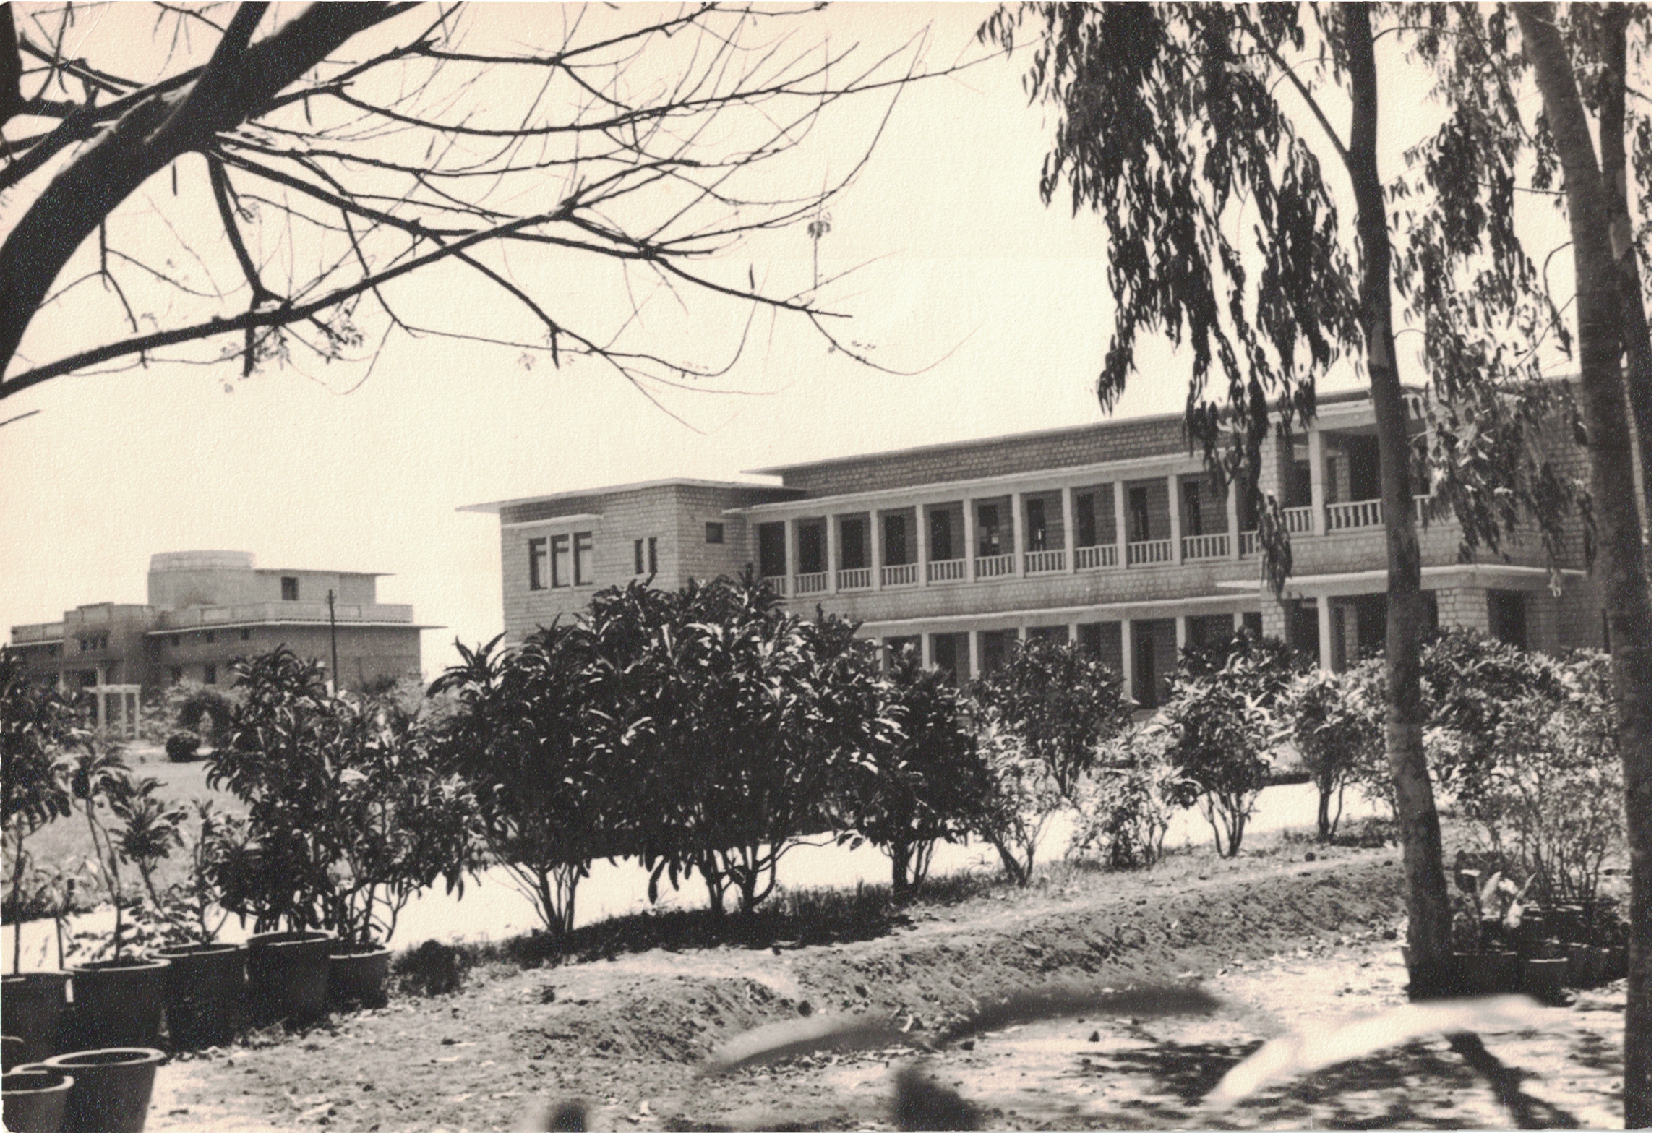
\includegraphics{"images/7.jpg"}
\caption{\enginline{1953}ರ ರಲ್ಲಿ ರಾಮನ್ ರಿಸರ್ಚ್ ಇನ್ಸ್ಟಿಟ್ಯೂಟ್}\label{chap2-fig01}
\end{sidewaysfigure}

ಅವರು ನಗುತ್ತಾ ಹೀಗೆ\enginline{-} “ಬಹುಶಃ ಸರ್ ಹಂಪ್ರಿಡೇವಿಯವರಿಗೆ ಫಾರಡೇ ಇದ್ದಂತೆ ನೀನೂ ಆಗಬಹುದು”. ಇದು ನನ್ನ ಜೀವನಕ್ಕೆ ಒಂದು ಮಹತ್ವದ ತಿರುವು ನೀಡಿತು. ಅತಿ ಸಂತೋಷಕರ ಗುರಿ ಮುಟ್ಟಿತು. ಈ ಬಗೆಯ ತಿರುವು ಅದುವರೆವಿಗಾಗಲಿ, ಆನಂತರವಾಗಲಿ ನನ್ನ ಜೀವನದಲ್ಲಿ ಬಂದಿಲ್ಲ. ಈ ಶತಮಾನದ ಅತಿ ಹಿರಿಯ ವಿಜ್ಞಾನಿಯ ಜೊತೆ ಸಂಪರ್ಕ ಪಡೆದು, ನನ್ನ ಹೃದಯಕ್ಕೆ ಹತ್ತಿರವಾದ ಪಥದಲ್ಲಿ ಸಾಗಲು ಅಣಿ ಮಾಡಿದ ತಿರುವು. ನಾನು ಹಿಂತಿರುಗಿ ನೋಡಿದಾಗ ನಾನು ಸಹಿಸಿದ ನಿರಾಶೆಗಳೆಲ್ಲವೂ ಒಳ್ಳೆಯದಕ್ಕೇ ಆದವು ಎನಿಸುತ್ತದೆ. ಈ ಘಟನೆ ನಡೆದದ್ದು ನವೆಂಬರ್ \enginline{1, 1949}ರಲ್ಲಿ ರಾಮನ್‍ರವರು ತಕ್ಷಣವೇ ಬೆರಳಚ್ಚುಗಾರರಿಗೆ ಉದ್ಯೋಗ ಪತ್ರದ ಒಕ್ಕಣೆ ನೀಡಿದರು. ಅದನ್ನು ಸಹಿ ಮಾಡಿ ನನ್ನ ಕೈಗಿತ್ತರು. ನನಗೆ ಕೆಲಸಕ್ಕೆ ಸೇರಲು ಹತ್ತು ದಿನಗಳ ಕಾಲಾವಧಿ ನೀಡಿದರು. ಅವರು ನನ್ನನ್ನು ಬಸ್‍ಸ್ಟಾಂಡಿನ ವರೆಗೆ ತಂದು ಬಿಟ್ಟರು. ನಾನು ಮದರಾಸಿಗೆ ಅದೇ ರಾತ್ರಿ ರೈಲು ಹತ್ತಿದೆ. ಒಂದು ವಾರ ನನ್ನ ಹಳ್ಳಿಯಲ್ಲಿ ಕಳೆದು, ಬೆಂಗಳೂರಿನ ಕೆಲಸಕ್ಕೆ ಹಾಜರಾದೆ. ನನಗೆ ಮುಂಚೆ ಬೆರಳಚ್ಚುಗಾರ ಬಾಲಕೃಷ್ಣನ್ ಮತ್ತು ಪದ್ಮನಾಭನ್‍ರವರುಗಳು ಕೆಲಸಕ್ಕೆ ಸೇರಿದ್ದರು. ರಾಮನ್ ಸಂಸ್ಥೆಯ ಕೆಲಸ ಶುರುವಾಗಿದ್ದು ಇಲ್ಲಿಂದಾಚೆಗೆ.

ರಾಮನ್‍ರವರು ಸಂಸ್ಥೆಗೆ ಬೇಕಾದ ಸಲಕರಣೆಗಳನ್ನೂ ಇತರೆ ಸಾಮಾನು ಸರಂಜಾಮುಗಳನ್ನು ಕೂಡಿಹಾಕತೊಡಗಿದರು. ಅವರು ಅನೇಕ ಸೂಕ್ಷ್ಮದರ್ಶಕಗಳನ್ನೂ, ರೂಮಿನ ತುಂಬ ಎಲೆಕ್ಟ್ರಾನಿಕ್ ಉಪಕರಣಗಳನ್ನೂ ಜೋಡಿಸಿದ್ದರು (ಇವು ಅಮೆರಿಕದ ಮಿಲಿಟರಿಯವರ ಉಪಕರಣಗಳು, ಯುದ್ಧ ಮುಗಿದ ಬಳಿಕ ಇಂತಹವನ್ನು ಶೈಕ್ಷಣಿಕ ಸಂಸ್ಥೆಗಳಿಗೆ ಮತ್ತು ಸಂಶೋಧನಾ ಸಂಸ್ಥೆಗಳಿಗೆ \enginline{DGTD}ಯು ಕೊಡಮಾಡಿತ್ತು) ಇವುಗಳಲ್ಲಿ ಮ್ಯಾಗ್ನೆಟೋಟ್ರಾನ್, ಸೂಕ್ಷ್ಮತರಂಗೋತ್ಪಾದಕ, ಆಂದೋಲಿಗಳು\break ವಿದ್ಯುತ್ ಅಲೆಗಳ ಸಲಕರಣೆಗಳು, ಏರಿಯಲ್ ಕ್ಯಾಮೆರಾಗಳು, ದ್ಯುತಿಉಪಕರಣಗಳು, ಅವಕೆಂಪು ವೀಕ್ಷಣಾ ಸಾಧನೆಗಳು ಸೇರಿದ್ದವು. ಮೆಷೀನ್ ಟೂಲ್‍ಗಳು, ಲೇಥ್‍ಗಳು, ನೈಟ್ರೋಜನ್ ದ್ರವೀಕರಣ ಉಪಕರಣಗಳು ಈ ದೇಣಿಗೆಯಲ್ಲಿ ಅದೃಷ್ಟವಶಾತ್ ಸೇರಿಕೊಂಡಿದ್ದವು.

ರಾಮನ್‍ರವರ ಕೊನೆಯ ಮಗ ರಾಧಾಕೃಷ್ಣನ್ ಈ ಉಪಕರಣಗಳ ಆಯ್ಕೆಯಲ್ಲಿ ಸಹಾಯ ಮಾಡಿದ್ದರು. ಅವರು ಹವ್ಯಾಸಿ ರೇಡಿಯೋ ತಜ್ಞರಾಗಿದ್ದರು. ಆದರೆ ಹೀಗೆ ಬಂದುವೆಲ್ಲಾ ಕಾರ್ಯನಿರತ ಸ್ಥಿತಿಯಲ್ಲಿರಲಿಲ್ಲ. ಕೆಲವು ಮೆಷಿನ್‍ಗಳ ಟೂಲ್ಸ್ ಮತ್ತು ಬೆಳಕಿನ ಉಪಕರಣಗಳು ಮಾತ್ರ ಕೆಲಸ ಮಾಡುತ್ತಿದ್ದವು. ಪಶ್ಚಿಮದ ಬಯಲಿನಲ್ಲಿ ಇವಕ್ಕೆ ದೊಡ್ಡದೊಂದು ಕಟ್ಟಡ ಕಟ್ಟಿಸಿ ಅಲ್ಲಿ ಲೇಥ್‍ಗಳು, ಮೇಷೀನುಗಳು, ಗಾಜುಊದುವ ತಂತ್ರಜ್ಞಾನ, ರಾಸಾಯನಿಕ ಲ್ಯಾಬ್, ಇತ್ಯಾದಿಗಳಿಗೆ ಅವಕಾಶ ನೀಡಲಾಯಿತು.

ಮುಖ್ಯ ಕಟ್ಟಡದ ಪೂರ್ವಕ್ಕೆ ರೋಹಿತದರ್ಶಕ ಪ್ರಯೋಗಾಲಯ ಕಟ್ಟಲಾಯಿತು. ಕಟ್ಟಡಗಳ ವಿಚಾರ ಬಂದಾಗ ರಾಮನ್‍ರವರಿಗೆ ಅವೆಲ್ಲವೂ ನಯಗೊಳಿಸಿದ ಗ್ರಾನೈಟ್‍ನಲ್ಲಿರಬೇಕೆಂದು ಇಷ್ಟ. ಅವುಗಳ ವಿನ್ಯಾಸದ ಬಗ್ಗೆಯೂ ಅವರಿಗೆ ನಿಶ್ಚಿತವಾದ ಅಭಿಪ್ರಾಯಗಳಿದ್ದವು. ಮುಖ್ಯ ಕಟ್ಟಡವು ಹೇಗಿರಬೇಕೆಂದು ಯೋಚಿಸಿದ್ದರು. ಪ್ರತಿಯೊಂದು ರೂಮನ್ನು ಹೇಗೆ ಬಳಸಬೇಕೆಂದು ಯೋಚಿಸಿದ್ದರು. ಮುಖ್ಯ ಕಟ್ಟಡಗಳಲ್ಲಿ ಪ್ರಯೋಗಾಲಯ, ಗ್ರಂಥಾಲಯ, ಸಂಗ್ರಹಾಲಯ, ಕಚೇರಿಗಳು,\break ವಾಚನಾಲಯ ಮತ್ತು ಬಾತ್‍ರೂಂಗಳಿರಬೇಕೆಂದು ಅವರು ಸ್ಥಳಾವಕಾಶ ಮಾಡಿದ್ದರು.\break ಸಂಗ್ರಹಾಲಯದ ಪಕ್ಕದಲ್ಲಿದ್ದ ಅವರ ಖಾಸಗಿ ವಾಚನಾಲಯವು ಅದ್ಭುತವಾಗಿತ್ತು, ಸುತ್ತಲೂ ಟೀಕ್\-‍ಮರದ ಹೊದಿಕೆ ಹಾಕಿ, ತೇಗದ ಬುಕ್ ಶೆಲ್ಫ್‌ಗಳಿದ್ದವು. ಮೂಲೆಗಳಲ್ಲಿ ಖನಿಜಗಳ ಮಾದರಿಗಳನ್ನು ಇಟ್ಟ ಶೋಕೇಸ್‍ಗಳಿದ್ದವು. ಒಂದು ದೊಡ್ಡ ತೇಗದ ಮರದ ಮೇಜು ಕೊಠಡಿಯ ಕೇಂದ್ರದಲ್ಲಿತ್ತು. ಇದರ ಮೇಲೆ ಕರಿಯ ಗಾಜಿನಫಲಕ ಇರಿಸಿದ್ದರು. ಸುತ್ತಲೂ ಆರಾಮ ಖುರ್ಚಿಗಳಿದ್ದವು. ಕೆಂಪೇಗೌಡ ಗೋಪುರವನ್ನು ಪೂರ್ವದ ಕಡೆಯೂ, ಪ್ಯಾಲೇಸ್ ಗಾರ್ಡ್‌ನ್‍ಗಳನ್ನು ದಕ್ಷಿಣದ ಕಿಟಕಿಗಳ ಮೂಲಕವೂ ನೋಡ ಬಹುದಿತ್ತು. ಅತ್ಯಂತ ಶ‍್ರೀಮಂತವಾಗಿ ಅನುಗೊಳಿಸಿದ ಚೆಂದವಾದ ರೂಂ ಆಗಿತ್ತು. ಅನೇಕ ಪುಸ್ತಕಗಳು ಮತ್ತು ಪತ್ರಿಕೆಗಳನ್ನು ಅಲ್ಲಿ ಜೋಡಿಸಲಾಗಿತ್ತು. ರಾಮನ್‍ರವರಿಗೆ ಇದು ವಾಚನಾಲಯ. ಅಲ್ಲೇ ಅವರು ತಮ್ಮ ಸಂದರ್ಶಕರನ್ನು ಎದುರುಗೊಳ್ಳುತ್ತಿದ್ದರು. ಪಕ್ಕದ ಸಣ್ಣ ರೂಂನಲ್ಲಿ ಅವರಿಗೆ ನೀಡಿದ ನೆನಪಿನ ಕಾಣಿಕೆಗಳನ್ನು ಪ್ರದರ್ಶಿಸಿದ್ದರು. ಎಲ್ಲವೂ ಅಚ್ಚುಕಟ್ಟಾಗಿ ಜೋಡಿಸಿ ಸಂಖ್ಯೆಗಳನ್ನು ಅಂಟಿಸಿದ್ದರು. ವಾಚನಾಲಯದಿಂದ ಒಳಬರಲು ಇದಕ್ಕೆ ಬಾಗಿಲಿತ್ತು. ಕೆಳಮಹಡಿಯಲ್ಲಿ ಈಶಾನ್ಯ ಮೂಲೆಯಲ್ಲಿ ರಾಮನ್‍ರವರ ಖಾಸಗಿ ಕಚೇರಿ ಇತ್ತು. ಇದು ಅವರ ಆಡಳಿತ ಕಛೇರಿಯ ಪಕ್ಕದಲ್ಲೇ ಇತ್ತು. ಅಲ್ಲಿ ಅವರ ಕಚೇರಿ ಸಿಬ್ಬಂದಿಗಳು ಇರುತ್ತಿದ್ದರು. ರಾಮನ್‍ರವರು ಖಾಸಗಿ ಕೊಠಡಿಯಲ್ಲಿ, ತಮ್ಮ ಪೂರ್ಣ ಖಾಸಗಿ ಸಂಗ್ರಹವನ್ನು ಇಟ್ಟಿದ್ದರು \enginline{-} ಅವರ ನೆನಪಿನ ಕಾಣಿಕೆಗಳು, ಮೆಡಲ್‍ಗಳು, ಡಿಪ್ಲೊಮಾಗಳು, ಡಾಕ್ಟೊರಲ್ ಗೌನ್‍ಗಳು, ವಜ್ರಗಳು ಮತ್ತು ಇತರ ಸ್ಫಟಿಕಗಳು ಇತ್ಯಾದಿ. ಅವರು ಫೋನ್‍ಕಾಲ್ ತೆಗೆದುಕೊಳ್ಳುವುದೂ, ಪತ್ರವ್ಯವಹಾರ ಮಾಡುವುದೂ, ಆಡಳಿತ ವಿಚಾರಗಳನ್ನು ನೋಡಿಕೊಳ್ಳುವುದೂ ಇಲ್ಲಿಯೆ ಜರುಗುತ್ತಿದ್ದವು.

ರಾಮನ್‍ರವರು ಟಾಟಾ ವಿಜ್ಞಾನ ಸಂಸ್ಥೆಯಿಂದ ನಿವೃತ್ತರಾಗುವ ಮೊದಲು ಅಮೆರಿಕ ದೇಶಕ್ಕೆ ಎರಡು ಬಾರಿ ಹೋಗಿದ್ದರು. ವಿಶ್ವ ಬ್ಯಾಂಕ್‍ನ ಕಛೇರಿಗೆ ಭಾರತದ ಪರವಾಗಿ ಹೋಗುವ ಸಂದರ್ಭವಿದ್ದು, ಅವರು ಭಾರತ ತಂಡದ ಸದಸ್ಯರಾಗಿ ಏನು ಮಾಡಿದರೆಂಬ ಮಾಹಿತಿಯು ಇಲ್ಲ. ಆದರೆ ಅವರು ಈ ಸಂದರ್ಭವನ್ನು ಅಮೆರಿಕದ ಅನೇಕ ವಿಜ್ಞಾನ ಸಂಸ್ಥೆಗಳನ್ನು ಸಂದರ್ಶಿಸಲು ಬಳಸಿಕೊಂಡರು. ಅವರು ಬೆಲ್ ಲ್ಯಾಬೊರೇಟರಿ ಮತ್ತು ಮುರ್ರೆಹಿಲ್‍ಗಳಿಗೆ ಹೋಗಿದ್ದರು. ಅಮೆರಿಕದ ಅನೇಕ ವ್ಯಾಪಾರಿಗಳ ಬಳಿ ಬಹು ಮೌಲ್ಯದ ವಜ್ರಗಳನ್ನು, ಖನಿಜಗಳನ್ನು ಕೊಂಡು\-ಕೊಂಡರು. ರಾಮನ್ ಸಂಸ್ಥೆಗೆ ಸೇರುವಾಗಲೇ ಇವೂ ಕೂಡ ಅಮೇರಿಕದಿಂದ ಬಂದಿಳಿದವು. ಸ್ಫಟಿಕಗಳ, ಖನಿಜಗಳ, ವಜ್ರ ರತ್ನಗಳ ಮತ್ತು ಭೂಗರ್ಭಶಾಸ್ತ್ರ ವಿಷಯಗಳ ಸುಸಜ್ಜಿತ ಸಂಗ್ರಹಾಲಯಕ್ಕೆ ರಾಮನ್‍ರವರ ಬಳಿ ಒಳ್ಳೆಯ ಯೋಜನೆಗಳಿದ್ದವು. ಮೊದಲ ಮಹಡಿಯಲ್ಲಿ ಅನೇಕ ಕೊಠಡಿಗಳನ್ನು ಮೀಸಲಾಗಿಟ್ಟಿದ್ದರು. ಅವರು ಈ ಕೊಠಡಿಗಳನ್ನು ಚೆನ್ನಾಗಿ ಸಜ್ಜುಗೊಳಿಸಲು ಈ.ಕೆ.ಗೋವಿಂದರಾಜ್\-‍ರವರನ್ನು ಬರಮಾಡಿಕೊಂಡರು. ಇವರು ಛಾಯಾಚಿತ್ರ ವಹಿವಾಟುದಾರರು ಮತ್ತು ಛಾಯಾಚಿತ್ರ ಸಂಬಂಧಿ ಉಪಕರಣಗಳನ್ನು ಮಾರುತ್ತಿದ್ದರು. ಗೋವಿಂದರಾಜ್‍ರವರಿಗೆ ಸೌಂದರ್ಯ ಪ್ರಜ್ಞೆ ಇತ್ತು. ಅವರು ಟೀಕ್ ಬೀರುಗಳನ್ನೂ, ಸರಿಯುವ ಗ್ಲಾಸ್ ಬಾಗಿಲುಗಳನ್ನು ಇರಿಸಿ ಬೆಳಕು ಒಳಗಡೆ ಬೀಳಬೇಕೆಂದು ಸಲಹೆ ಮಾಡಿದರು. ಬೀರುಗಳೊಳಗೆ ಶೆಲ್ಫ್‌ಗಳು ಶೀಟ್ ಗ್ಲಾಸ್‍ನಿಂದ ಇರಬೇಕೆಂದರು. ಟೀಕ್ ಮರದ ಪಟ್ಟಿಗಳಲ್ಲಿ ಚಿತ್ರಗಳ ವಿನ್ಯಾಸಗಳಿದ್ದು ಅದಕ್ಕೆ ಮರದ ತೊಗಟೆಯ ಗೆರೆಗಳು ಎದ್ದು ಕಾಣುವಂತೆ ಪಾಲಿಷ್ ಮಾಡಲಾಗಿತು. ಗೋವಿಂದರಾಜ್ ಬಡಗಿಗಳನ್ನು ಕರೆಸಿ ಸಂಸ್ಥೆಯಲ್ಲೇ ಬೀರುಗಳನ್ನು ಮಾಡಿಸಿ ಜೋಡಿಸಿದರು. ಪ್ರತಿಯೊಂದು ಹಂತದಲ್ಲಿಯೂ ರಾಮನ್‍ರವರ ಸಲಹೆ ಕೋರುತ್ತಿದ್ದರು. ಅವರ ಸಮ್ಮತಿ ಪಡೆಯುತ್ತಿದ್ದರು. ರಾಮನ್‍ರವರಿಗೆ ಇಷ್ಟವಾಗದ್ದನ್ನು ಗೋವಿಂದರಾಜ್‍ಗೆ ತಿಳಿಸುತ್ತಿದ್ದರು. ರಾಮನ್ ಹೇಳಿದಂತೆಯೇ ಕೆಲಸಗಳಾಗುತ್ತಿದ್ದವು. ಗೋವಿಂದರಾಜ್ ಬಹಳ ಚುರುಕು. ಬಹುಬೇಗನೇ ರಾಮನ್‍ರವರ ಇಷ್ಟ/ಅನಿಷ್ಟಗಳನ್ನು ತಿಳಿದುಕೊಂಡು ಬಿಟ್ಟರು. ಶೆಲ್ಫ್‌ಗಳನ್ನು ಕೂಡಿಸಿದ ಮೇಲೆ ರಾಮನ್ ಅವುಗಳೊಳಗೆ ಮೇಲೆ ಮಾದರಿಗಳನ್ನಿಡಲು ಬಹಳ ಮುತುವರ್ಜಿ ವಹಿಸಿದರು. ಮೊದಲ ಮಹಡಿಗೆ ಮಾದರಿಗಳನ್ನು ಒಂದೊಂದಾಗಿ ಅವರೇ ಕೈಯಾರ ತೆಗೆದುಕೊಂಡು ಹೋಗುತ್ತಿದ್ದರು. ನಾವು ಅವರಿಗೆ ಬಹಳ ಸಹಾಯ ಮಾಡಿದೆವು. ನಮ್ಮನ್ನು ಸುತ್ತಲೂ ನಿಲ್ಲಿಸಿಕೊಂಡು ಮಾದರಿಗಳನ್ನು ಜೋಡಿಸಿ ನಮಗೆ ತೋರಿಸಿ “ಈಗ ಹೇಗೆ ಕಾಣುತ್ತದೆ” ಎಂದು ಪ್ರತಿಬಾರಿಯೂ ಕೇಳುತ್ತಿದ್ದರು. ಹೀಗೆ ಪ್ರತಿ ಮಾದರಿಯನ್ನು ಜೋಡಿಸಲು ಬಹಳ ಸಮಯ ತಗಲುತ್ತಿತ್ತು. ಅವರಿಗೆ ಕಾಳಜಿಯಿದ್ದದ್ದು ಪ್ರತಿಯೊಂದು ಮಾದರಿಯ ಮೇಲೆ ಬೆಳಕು ಬಿದ್ದು ಅದು ಸುಂದರವಾಗಿ ಬೆಳಗಬೇಕು ಎಂದು. ಈ ಪ್ರಕ್ರಿಯೆಗಳು ಗಂಟೆಗಟ್ಟಲೇ ನಡೆಯುತ್ತಿದ್ದವು. ನಾವು ರಾಮನ್‍ರವರ ಸಹವಾಸವನ್ನು ಬಹಳವಾಗಿ ಸಂತೋಷಪಟ್ಟು ಬಯಸುತ್ತಿದ್ದೆವು. ಅವರ ವ್ಯಾಖ್ಯೆಗಳನ್ನು ಕೇಳುತ್ತಿದ್ದೆವು. ಅವರು ಮಾದರಿಗಳಿಗೆ ಹೆಸರು ನಮೂದಿಸಲು ಸಮ್ಮತಿಸುತ್ತಿರಲಿಲ್ಲ, ಅವನ್ನೆಲ್ಲ ತೆಗೆದಿರಿಸಿದರು. ಇವುಗಳ ಹೆಸರುಗಳನ್ನು ತಮ್ಮ ತಲೆಯಲ್ಲಿ ತುಂಬಿಕೊಂಡಿದ್ದರು. ರಾಮನ್‍ರವರಿಂದ ಉಂಟಾದ ಈ ತರಬೇತಿಯಲ್ಲಿ ನಾನು ಮತ್ತು ಪದ್ಮನಾಭನ್ ನಿರಂತರವಾಗಿ ಇದ್ದುದ್ದರಿಂದ ಪ್ರತಿಯೊಂದು ಖನಿಜ, ಮಾದರಿಯ ಹೆಸರುಗಳನ್ನೂ, ಅವುಗಳು ರಾಮನ್‍ರಿಗೆ ಸಿಕ್ಕಿದ ಬಗೆಯ ಚರಿತ್ರೆಯನ್ನು ಬಾಯಿಪಾಠ ಮಾಡಿದೆವು.

ಅತಿವರ್ಣರಂಜಿತ ಹೊಳಪಿನ ಸ್ಫಟಿಕಗಳನ್ನು ನೇರ ಹಾಗೂ ಪಾರ್ಶ್ವದಿಂದ ಬೆಳಕು ನುಗ್ಗುವ ಮೂಲೆ ಕೊಠಡಿಯಲ್ಲಿ ಇಟ್ಟೆವು. ಬೆಸ್ಸೇಸರ್ ಲಾಲ್ ಹಲ್ವಾಸಿಯಾ ಮ್ಯೂಸಿಯಂ ವಿಶಾಲವಾಗಿತ್ತು. ಇಲ್ಲಿ ಅತಿ ದೊಡ್ಡ ಗಾತ್ರದ ಖನಿಜ ಮಾದರಿಗಳನ್ನು ಇಟ್ಟೆವು. ಇದರಲ್ಲಿ ತೇಗದ ಮರದ ಉದ್ದನೆಯ ಕಪಾಟಿತ್ತು. ಇದಕ್ಕೆ ಗಾಜಿನ ಛಾವಣಿಯೂ ಸರಿಸಮ ದ್ವಾರಗಳೂ ಇದ್ದವು. ಇಲ್ಲಿ ಸ್ಫಟಿಕಗಳನ್ನು ಮತ್ತು ಕೃತಕ ವಜ್ರಗಳನ್ನು ಇರಿಸಿದ್ದೆವು. ಮೂಲೆಯ ರೂಮಿನ ಪಕ್ಕದಲ್ಲಿ ಇನ್ನೊಂದು ಸಣ್ಣ ಕೊಠಡಿ ಇತ್ತು. ಅದರಲ್ಲಿ ಅತಿ ನೇರಳೇ ಕಿರಣಗಳಲ್ಲಿ ದೀಪ್ತಿಸೂಸುವ ಖನಿಜಗಳನ್ನು ಪ್ರದರ್ಶನಕ್ಕೆ ಇದ್ದವು. ಪ್ರಕಾಶಮಾನವಾದ ಹಸಿರು ವಿಲ್ಲೆಮೈಟ್, ಕೆಂಪು ಕಾಲ್ಸೈಟುಗಳು, ನೀಲಿ ಫ್ಲೂರ್‍ಸ್ಟಾರ್ ಮತ್ತು ನ್ಯೂಜರ್ಸಿಯಿಂದ ತಂದ ಹಲವು ವರ್ಣಗಳ ಫ್ರಾಂಕ್‍ಲೈನೈಟ್ ಇವು ಪ್ರದರ್ಶನಕ್ಕೆ ಇಟ್ಟ ಕೆಲವು ಖನಿಜಗಳು. ಇವು ಕತ್ತಲಕೋಣೆಯಲ್ಲಿದ್ದು, ಅತಿನೀಲ ಬಲ್ಬ್ ಹೊತ್ತಿಕೊಂಡಾಗ ಜೀವ ಪಡೆಯುತ್ತಿದ್ದೆವು. ರಾಮನ್ ಈ ಖನಿಜಗಳನ್ನು ಬಿಳಿ ಬೆಳಕಿನಲ್ಲಿ ಮೊದಲು ತೋರಿಸಿ, ಬಳಿಕ ಅತಿನೀಲ ಬೆಳಕಿನಲ್ಲಿ ಜಗಮಗಿಸುವ ಹಾಗೆ ಮಾಡುತ್ತಿದ್ದರು. ಇದರಿಂದ ದರ್ಶಕರಿಗೆ ವ್ಯತ್ಯಾಸ ತಿಳಿಯುತ್ತಿತ್ತು; ಮಾಯಾ ಲೋಕಕ್ಕೆ ಕರೆದೊಯ್ದಂತೆ ಇರುತ್ತಿತ್ತು. ಆಗ ರಾಮನ್‍ರವರು ದೀಪ್ತಿಯೆಂದರೇನು ಎಂದು ವಿವರಿಸುತ್ತಿದ್ದರು. ಈ ರೂಂನಲ್ಲಿ ನಡೆಯುವ ಮಾಯೆಯನ್ನು ಸಂದರ್ಶಕರು ತಮ್ಮ ನೆನಪಿನಲ್ಲಿ ಕೊಂಡೊಯ್ಯುತ್ತಿದ್ದರು. ಪಶ್ಚಿಮದ ಭಾಗದಲ್ಲಿ ಭೂವಿಜ್ಞಾನಕ್ಕೆ ಮೀಸಲಿರಿಸಿದ್ದರು (ಶಿಲೆಗಳು ಮತ್ತು ಶಿಲೆಗಳನ್ನುಂಟು ಮಾಡುವ ಖನಿಜಗಳು). ಇದರ ಬಳಿಕ ಎರಡು ಕೊಠಡಿಗಳಲ್ಲಿ ಚಿಟ್ಟೆಗಳು, ಜೀರಂಗಿಗಳು, ಹಕ್ಕಿಗಳು ಮತ್ತು ಹೊಳೆಯುವ ಕಪ್ಪೆಚಿಪ್ಪುಗಳಿದ್ದವು.

ಹೀಗೆ ರಾಮನ್ ತಮ್ಮ ಸಂಸ್ಥೆಯನ್ನು ಸಂಗ್ರಹಾಲಯಗಳು, ಉಪನ್ಯಾಸ ಕೊಠಡಿ, ಗ್ರಂಥಾಲಯ, ಕಚೇರಿ ಮತ್ತು ಪ್ರಯೋಗಾಲಯಗಳಿಂದ ಸಜ್ಜುಗೊಳಿಸಿ ತಮ್ಮ ಬೆಟ್ಟದಷ್ಟು ಉತ್ಸಾಹ ಮತ್ತು\break ಕಾರ್ಯಶೀಲತೆಯಿಂದ ಕೆಲಸಕ್ಕೆ ತೊಡಗುತ್ತಿದ್ದರು. ಅವರು ಕೆಲವು ಸಂಶೋಧಕ ವಿದ್ಯಾರ್ಥಿಗಳನ್ನು ತೆಗೆದುಕೊಂಡರಾದರೂ, ಮುಖ್ಯವಾಗಿ ಈ ಸಂಸ್ಥೆಯು ಅವರು ತೊಡಗಿಸಿಕೊಳ್ಳ ಬಯಸುವ ವಿಜ್ಞಾನ ರಂಗಗಳಲ್ಲಿಯೇ ಸಂಶೋಧನೆಗೆ ತೊಡಗಿತ್ತು.

ರಾಮನ್‍ರವರಿಗೆ ಶ‍್ರೀಮಂತರ ಅಭಿರುಚಿಗಳಿದ್ದವು. ರಾಮನ್ ಸಂಸ್ಥೆಯ ಆವರಣದಲ್ಲಿ ನೆಲಮಟ್ಟದ ಹೂ ತೋಟವಿರಬೇಕೆಂದೂ ಹಸಿರು ಚಪ್ಪರದ ಹಾದಿಯಿರಬೇಕೆಂದು ಮತ್ತು ಅಲ್ಲಿಯೇ ತಮಗೊಂದು ವಸತಿ ಇರಬೇಕೆಂದು ಬಯಸಿದರು. ಇದಕ್ಕಾಗಿ ಮಹಾರಾಜರಲ್ಲಿಗೆ ಮತ್ತೆ ಸಾರಿದರು. ತಮ್ಮ ಸಂಸ್ಥೆಯ ದಕ್ಷಿಣಕ್ಕೆ ಇರುವಂತೆ ನಾಲ್ಕು ಎಕರೆ ಭೂಮಿಯನ್ನು ಕೋರಿದರು. ಇದು ಕೃಷಿ ಭೂಮಿಯಾಗಿತ್ತು. ಮಹಾರಾಜರು ಇದನ್ನು ನೀಡಿದಾಗ ಅತಿಸಂತೋಷ ಪಟ್ಟರು. ಜಮೀನು ಸುಪರ್ದಿಗೆ ಬಂದ ತಕ್ಷಣ ಅದಕ್ಕೆ ಮುಳ್ಳುತಂತಿ ಬೇಲಿ ಹಾಕಿಸಿದರು. ಅನೇಕ ಗಿಡಗಳನ್ನು ಮತ್ತು ಮರಗಳನ್ನೂ ನೆಡೆಸಿದರು. ಇದರ ಬಳಿಕ ತಮ್ಮ ಕನಸಿನ ಮನೆಯನ್ನು ಕಟ್ಟಿಸಿದರು. ಇದು ಜಮೀನಿನ ಆಗ್ನೇಯ ಭಾಗದಲ್ಲಿತ್ತು. ಗ್ರಾನೈಟ್ ಶಿಲೆಯಲ್ಲಿ ಕಟ್ಟಿದ ನಿರ್ದೇಶಕರವರ ಬಂಗಲೆಯು ಒಂದು ಮಹಡಿಯುಳ್ಳ ಉದ್ದನೆಯ ಕಟ್ಟಡ. ಇದರ ದಕ್ಷಿಣಭಾಗದಲ್ಲಿ ನೆಲಮಟ್ಟದ ಹೂ ತೋಟವಿತ್ತು. ಇದರಲ್ಲಿ ಅತಿ ಸುಂದರ ಗುಲಾಬಿ ಗಿಡಗಳನ್ನು ಬೆಳೆಸಿದ್ದರು. ಬಂಗಲೆಯ ಪೂರ್ವದಲ್ಲಿ ಕೆಂಪೇಗೌಡರ ಉತ್ತರದ ಗೋಪುರವಿತ್ತು. ಇದು ಕೆಂಪು ಬಣ್ಣದ ಗುಡ್ಡದ ಮೇಲೆ ನಿಂತಿತ್ತು. ರಾಮನ್‍ರವರು ತಮ್ಮ ಬಂಗಲೆಯಲ್ಲಿ, ಮಲಗುವ ಕೋಣೆಯಿಂದ ಕೆಂಪೇಗೌಡ ಗೋಪುರವನ್ನು ನೋಡಬಹುದಿತ್ತು. ಹೂವಿನ ಚಪ್ಪರದ ಹಾದಿಗೆ ರಾಮನ್‍ರವರು ಹಳದಿ ಮತ್ತು ನೇರಳೆ ಬಣ್ಣದ ಹೂವಿನ ಬಳ್ಳಿಗಳನ್ನು ಆಯ್ದುಕೊಂಡರು. ಮನೆಯ ಮುಂದೆ ಕಾರು ನಿಲ್ಲಲು ಚಕ್ರಾಕಾರದ ಹಾದಿ ಮಾಡಿ ಗ್ರಾನೈಟ್‍ನಲ್ಲಿ ಪೋರ್ಟಿಕೋ ನಿರ್ಮಿಸಿದ್ದರು. ಬಂಗಲೆಯ ಪಶ್ಚಿಮಕ್ಕೆ ಅನೇಕ ನಡೆಹಾದಿಗಳನ್ನು ಹೂಗಿಡಗಳನ್ನು ಸೊಂಪಾಗಿ ಬೆಳೆಸಿದ್ದರು. ಒಟ್ಟಿನಲ್ಲಿ ಬಂಗಲೆಯು ಸುಂದರವಾಗಿ, ಹಸಿರು ಪರಿಸರದಲ್ಲಿತ್ತು.

ರಾಮನ್‍ರವರು ಇಷ್ಟೆಲ್ಲ ಸುಂದರ ಬಂಗಲೆ ಕಟ್ಟಿದ ಮೇಲೆ ಅಲ್ಲಿ ವಸತಿ ಮಾಡಲಿಲ್ಲ. ಮೂರು ಮೈಲಿ ದೂರದ ಮಲ್ಲೇಶ್ವರದ ಬಂಗಲೆಯಲ್ಲೇ ಇರುತ್ತಿದ್ದರು. ಈ ಬಂಗಲೆಯಲ್ಲಿ ವಾಸಕ್ಕೆ ಮೊದಲು ಬಂದವರು ಪಾಮರ್ ಕ್ರೈಗ್ ಎಂಬ ಅಮೇರಿಕದ ಇಲೆಕ್ಟ್ರಿಕಲ್ ಕಮ್ಯುನಿಕೇಶನ್‍ನ ಸಂದರ್ಶಕ ಪ್ರೊಫೆಸರ್. ಇವರು ಟಾಟಾ ವಿಜ್ಞಾನ ಸಂಸ್ಥೆಗೆ ಬಂದಿದ್ದರು. ಇದಾದದ್ದು ಹೀಗೆ, ಕ್ರೈಗ್‍ರವರು ಒಮ್ಮೆ ರಾಮನ್‍ರವರ ಬಳಿ ಬಂದಿದ್ದಾಗ ತಮ್ಮ ಮನೆ ಹುಡುಕುವ ಸಮಸ್ಯೆಯನ್ನು ಹೇಳಿಕೊಂಡರು. ರಾಮನ್ ತಮಾಷೆಗಾಗಿ ಹೀಗೆಂದರು “ನನ್ನ ಬಳಿ ಸುಂದರವಾದ ಬಂಗಲೆಯಿದೆ. ಆದರೆ ನಾನು ಹೇಳುವ ಬಾಡಿಗೆ ನೀವು ಕೊಡುವುದಿಲ್ಲವೆಂದು ಗೊತ್ತು”. ಕ್ರೈಗ್ ಬಾಡಿಗೆ ಎಷ್ಟು ಹೇಳಿ ಎಂದರು. ರಾಮನ್ ತಿಂಗಳಿಗೆ \enginline{2000} ರೂ ಎಂದರು. ಕ್ರೈಗ್ ಮನೆಯನ್ನು ನೋಡಿದರು. ತಕ್ಷಣವೇ ಅದೇ ಮೊತ್ತದ ಬಾಡಿಗೆ ನೀಡಲು ಮುಂದಾದರು. ಅಮೆರಿಕದಿಂದ ಬಂದ ಪ್ರೋಫೆಸರ್‍ಗೆ ಈ ಬಾಡಿಗೆ ಹೆಚ್ಚೆನಿಸಲಿಲ್ಲ. ಬಂಗಲೆಯೂ ಸುಂದರವಾಗಿತ್ತಲ್ಲ. ರಾಮನ್‍ರವರು ಸಿಕ್ಕಿಬಿದ್ದರು, ಕೊನೆಗೆ ಎರಡು ವರ್ಷದ ಮಟ್ಟಿಗೆ ಮನೆ ಬಾಡಿಗೆಗೆ ನೀಡಲು ಒಪ್ಪಿದರು. ಅಂದಿಗೆ ಅತಿ ಹೆಚ್ಚು ಮೊತ್ತವೆನಿಸಿದ ಬಾಡಿಗೆಯನ್ನು ತಮ್ಮ ಸಂಸ್ಥೆಯ ಒಳತಿಗಾಗಿ ಉಪಯೋಗಿಸಲು ಯೋಚಿಸಿದ್ದರು. ಆದರೆ ಎರಡು ವರ್ಷ ಹತ್ತಿರವಾಗುತ್ತಿದ್ದಂತೆಯೇ ಅವರಿಗೆ ಅಸಹನೆ ಮೂಡಿತು. ತಮ್ಮ ಬಂಗಲೆಯನ್ನು ಬಾಡಿಗೆಗೆ ಕೊಟ್ಟಿದ್ದೇ ತಪ್ಪು ಎಂದು ನನ್ನೊಡನೆ ಹೇಳಿದ್ದರು. ಹೆಚ್ಚಿನ ಬಾಡಿಗೆಯ ಆಸೆಗೆ ಬಾಯಿ ಬಿಡಬಾರದಾಗಿತ್ತು ಎಂದಿದ್ದರು.

ಸಂಸ್ಥೆಯ ಆವರಣದಲ್ಲಿ ಒಂದು ಹಾಸ್ಟಲ್ ಮತ್ತು ಎರಡು ಮನೆಗಳನ್ನು ಕಟ್ಟಲು ವ್ಯವಸ್ಥೆ ಮಾಡಿದರು. ಅವರು ನನ್ನ ವಾಸಕ್ಕಾಗಿ ಏನೇನು ಅನುಕೂಲತೆಗಳು ಬೇಕೋ ಅವನ್ನು ಈ ಮನೆಗಳ ವಿನ್ಯಾಸದಲ್ಲಿ ಅಳವಡಿಸಲು ಹೇಳಿದರು. “ನೀವು ಇಲ್ಲಿ ಸುಖವಾಗಿ, ತೊಂದರೆಯಿಲ್ಲದೆ ಇರಬೇಕು, ಬಾತ್‍ರೂಂಗಳಲ್ಲಿ ಗೀಸರ್, ವೆಸ್ಟ್ರ್‌ನ್ ಟಾಯ್‍ಲೆಟ್ ಇರಲಿ” ಎಂದು ಹೇಳಿದ್ದರು. ಅವರು ನನಗೆ ಈ ಮನೆಯನ್ನು ಬಾಡಿಗೆಯಿಲ್ಲದೆ ನೀಡಿದ್ದರು. ಸಂಸ್ಥೆಯ ಕ್ಯಾಂಪಸ್‍ನಲ್ಲಿರುವುದು ವೈಜ್ಞಾನಿಕ ಕಾರ್ಯ ಮಾಡಲು ಅನುಕೂಲವೆನಿಸಿದರೂ, ಅಂದಿನ ದಿನಗಳಲ್ಲಿ ಈ ಸ್ಥಳವು ನಾಗರಿಕತೆಯಿಂದ ಬಹಳ ದೂರವಿದೆಯೆಂದು ಅನಿಸುತ್ತಿತ್ತು. ಆದರೆ ಹವಾಮಾನ ಹಿತಕರವಾಗಿತ್ತು, ಸುತ್ತಮುತ್ತ ಸುಂದರ ಹಸಿರಿತ್ತು. ನಾನು, ನನ್ನ ಕುಟುಂಬ, ಇಂಡಿಯನ್ ಅಕಾಡೆಮಿ ಆಫ್ ಸೈನ್ಸ್‌ಸ್‍ನ ಮ್ಯಾನೇಜರ್ ವೆಂಕಟಾಚಾರ್ ಕುಟುಂಬ ಮತ್ತು ಇತರ ಸಂಶೋಧಕರು ಒಂದೇ ಕುಟುಂಬದವರಂತೆ ಇದ್ದೆವು. ಅಲ್ಲಿನ ಗಾಳಿ ಬೆಳಕನ್ನು ಊರ ಹೊರಗಿನ ತಾಪತ್ರಯಗಳನ್ನು ಒಟ್ಟಿಗೇ ಅನುಭವಿಸಿದೆವು.

ರಾಮನ್‍ರವರು ಕ್ಯಾಂಪಸ್‍ನಲ್ಲಿ ನಿರ್ದೇಶಕ ಬಂಗಲೆಗೆ ವಾಸಕ್ಕೆ ಬರುವ ಮೊದಲು, ಮಲ್ಲೇಶ್ವರಂ\-ನಲ್ಲಿದ್ದ ದೊಡ್ಡ ಮನೆಯಲ್ಲಿ ವಾಸವಾಗಿದ್ದರು. ಮನೆಯ ಹೆಸರು ಪಂಚವಟಿ (ಅಂದರೆ ಆಶ್ರಮ) ಅದರಲ್ಲಿ ಬೇವು, ಮಾವು, ಹಲಸು ಮತ್ತು ಇತರ ಮರಗಳಿದ್ದವು. ಈ ಮನೆಯನ್ನು ಬಹಳ ಚೌಕಾಸಿ ಮಾಡಿ ಕಡಿಮೆ ಬೆಲೆಗೆ ರಾಮನ್ ಕೊಂಡಿದ್ದರು. ಒಂದು ಕಥೆಯ ಪ್ರಕಾರ ಈ ಮನೆಯಲ್ಲಿ ದೆವ್ವದ ಕಾಟವಿತ್ತಂತೆ, ಅದಕ್ಕೆ ಇದನ್ನು ಕೊಳ್ಳಲು ಯಾರೂ ಮುಂದೆ ಬರುತ್ತಿರಲಿಲ್ಲವಂತೆ. ರಾಮನ್‍ಗೆ ಇದು ಗೊತ್ತಾದಾಗ, ನಾನು ಅದಕ್ಕಿಂತಲೂ ದೊಡ್ಡದೆವ್ವ; ಅದೇ ಮನೆ ಬಿಟ್ಟು ಹೋಗ ಬೇಕಷ್ಟೆ ಎಂದಿದ್ದರಂತೆ.

ಬೆಂಗಳೂರಿಂದ ಎಂಟು ಮೈಲಿ ದೂರದ ಕೆಂಗೇರಿಯಲ್ಲಿ ರಾಮನ್‍ರವರಿಗೆ \enginline{100} ಎಕರೆಯ ಎಸ್ಟೇಟ್ ಇತ್ತು. ಇಲ್ಲೊಂದು ಒಳ್ಳೆಯ ಬಂಗಲೆಯಿತ್ತು. ಕೃಷಿ ಭೂಮಿಯೂ, ನೂರಾರು ಮರಗಳೂ ಇದ್ದವು. ಇದರ ನೈರುತ್ಯ ಭಾಗದಲ್ಲಿ ತೊರೆಯೊಂದು ಹರಿಯುತ್ತಿತ್ತು. ಈ ಎಸ್ಟೇಟ್ ಅನ್ನು ವಾರದ ಕೊನೆಯಲ್ಲಿನ ವಿಶ್ರಾಂತಿಗಾಗಿ ಬಳಸುತ್ತಿದ್ದರು. ಅಲ್ಲಿ ನಡೆದಾಡುವುದೆಂದರೆ ಅವರಿಗೆ ಇಷ್ಟ. ಸಾಮಾನ್ಯವಾಗಿ ಶನಿವಾರ ಮಧ್ಯಾಹ್ನ ಅಲ್ಲಿಗೆ ಹೊರಡುತ್ತಿದ್ದರು. ಸಾಯಂಕಾಲದ ಸೂರ್ಯಾಸ್ತ ನೋಡುವುದು ಅವರಿಗೆ ಹವ್ಯಾಸವಾಗಿತ್ತು. ಎಸ್ಟೇಟ್‍ನ ನಿರ್ದಿಷ್ಟ ಜಾಗದಲ್ಲಿ ನಿಂತು ಸೂರ್ಯಾಸ್ತವನ್ನು ವೀಕ್ಷಿಸುತ್ತಿದ್ದರು. ಲೇಡಿ ರಾಮನ್ ಅವರೊಡನೆ ಇರುತ್ತಿದ್ದರು. ಅವರ ಬೇಕು ಬೇಡಗಳನ್ನು ನೋಡಿಕೊಳ್ಳುತ್ತಿದ್ದರು. ಬಂಗಲೆಯಲ್ಲಿ ಎಲ್ಲ ಅನುಕೂಲಗಳೂ ಇದ್ದವು. ಲೇಡಿ ರಾಮನ್‍ರವರು ಅಲ್ಲಿನ ನೌಕರರನ್ನು ನಿಬಾಯಿಸುತ್ತಿದ್ದರು. ಅಲ್ಲಿ ತರಕಾರಿ ಮತ್ತು ಇತರೆ ಧಾನ್ಯಗಳನ್ನೂ ಬೆಳೆಸುತ್ತಿದ್ದರು. ಭಾನುವಾರ ಬೆಳಿಗ್ಗೆ ರಾಮನ್‍ರವರು ಒಂದು ಉದ್ದನೆಯ ನಡಿಗೆಯ ಕಾರ್ಯಕ್ರಮ ಹಾಕಿಕೊಳ್ಳುತ್ತಿದ್ದರು. ಅವರಿಗೆ ಪ್ರಕೃತಿ ವೀಕ್ಷಣೆ ಬಹಳ ಮೆಚ್ಚು. ಅಲ್ಲಿ ಮಧ್ಯಾಹ್ನದ ಊಟ, ವಿಶ್ರಾಂತಿಗಳಾದ ನಂತರ ಹೊರಟು ಸಂಜೆಯ ವೇಳೆಗೆ ಬೆಂಗಳೂರಿಗೆ ಬರುತ್ತಿದ್ದರು. ರಾಮನ್‍ರವರು ಅಲ್ಲಿ ಒಂದು ಖಗೋಳವೇಧ ಶಾಲೆಯನ್ನು ತೆರೆಯಬೇಕೆಂದಿದ್ದರು.

ರಾಮನ್ ಸಂಸ್ಥೆಯ ಪೂರ್ವಕ್ಕೆ ಇದ್ದ ಐದು ಎಕರೆ ಜಮೀನನ್ನು ರಾಮನ್ ಕೊಳ್ಳಲು ಇಚ್ಚಿಸಿದರು. ಆಗ ಸಿಟಿ ಇಂಪ್ರೊವ್‍ಮೆಂಟ್ ಟ್ರಸ್ಟ್ ಬೋರ್ಡ್ ಇತ್ತು. ಮಹಾರಾಜರ ಎಲ್ಲಾ ಜಮೀನು ಇದರ ಕೈಯಲ್ಲಿತ್ತು. ಈ ಜಮೀನಿಗಾಗಿ \enginline{3,00,000/\general{\enginline{-}}} ರೂ ಕಟ್ಟಿದರು. ಕೆಂಪೇಗೌಡ ಗೋಪುರದ ಉತ್ತರ ಭಾಗದ ಸಟ್ಟುಮಣ್ಣಿನ ಗುಡ್ಡದ ಪ್ರದೇಶ ಇದು.

ಸಂಸ್ಥೆಯು ಬೆಳೆದಹಾಗೆಲ್ಲ ಈ ಜಾಗದಲ್ಲಿ ಕಟ್ಟಡಗಳನ್ನು ಕಟ್ಟಬೇಕೆಂದು ಯೋಚಿಸುತ್ತಿದ್ದರು. ಅಲ್ಲಿ ಹೊಸ ಗ್ರಂಥಾಲಯ ಕಟ್ಟಬೇಕೆಂದು ಅಡಿಪಾಯ ಹಾಕಿಸಿದ್ದರು. ಈ ಜಾಗದಲ್ಲಿ ಕಟ್ಟಡಗಳಿಲ್ಲದಿದ್ದರೆ ಸಿಟಿ ಬೋರ್ಡ್ ಜಾಗವನ್ನು ವಾಪಸ್ ತೆಗೆದುಕೊಳ್ಳಬಹುದೆಂಬ ಭಯವಿತ್ತು. \enginline{70}ರ ದಶಕದಲ್ಲಿ ರಾಮನ್ ತೀರಿಕೊಂಡ ಮೇಲೆ ಅಲ್ಲಿ ಹಲವಾರು ಕಟ್ಟಡಗಳು ಮೇಲೆದ್ದವು. ರೇಡಿಯೊ ಟೆಲಿಸ್ಕೋಪ್‍ನ ಕಟ್ಟಡವು ಠೀಕಾಗಿ ಎದ್ದು ಕಾಣುವಂತಾಯಿತು. ಈ ರೇಡಿಯೋ ದೂರದರ್ಶಕ ಮಿಲಿಮೀಟರ್ ತರಂಗಾಂತರದ್ದು. ರಾಮನ್‍ರವರ ದೂರದೃಷ್ಟಿಯು ಹೀಗೆ ಖುಜುವಾಯಿತು. ಈ ಜಾಗದ ಬೆಲೆ ಈಗ ಇನ್ನೂರು ಅಥವಾ ಮುನ್ನೂರು ಪಟ್ಟು ಹೆಚ್ಚಾಗಿದೆ. ಅಂದಿನ ಕಾಲದಲ್ಲಿ ರಾಮನ್ ಈ ಜಾಗವನ್ನು ಕೊಳ್ಳದಿದ್ದರೆ, ಸಂಸ್ಥೆಯು ವಿಜ್ಞಾನದ ಈ ಹೊಸರಂಗದಲ್ಲಿ ಕಾಲಿಡಲು ಅಸಾಧ್ಯವಾಗುತ್ತಿತ್ತು.

ರಾಮನ್‍ರವರು ಮದರಾಸಿನಲ್ಲಿಯೂ ಒಂದು ಬಡಾವಣೆಯಲ್ಲಿ ಜಮೀನಿನ ಮೇಲೆ ಹಣ ಹೂಡಿದ್ದರು. ನಗರದ ಈ ಭಾಗವು ಅತಿ ಶೀಘ್ರವಾಗಿ ಬೆಳೆದು, ಅದರ ಮೌಲ್ಯ ಹೆಚ್ಚಿತು. ಅಲ್ಲಿ ಬಂಗಲೆಯೊಂದನ್ನು ಕಟ್ಟಿ, ರಾಮನ್ ಸಂಸ್ಥೆಯ ಶಾಖೆಯೊಂದನ್ನು ತೆರೆಯಲು ಇಚ್ಚಿಸಿದ್ದರು. ಇಲ್ಲಿ ಗಣಿತ ಸಂಶೋಧನೆ ಮಾಡಲು ಉದ್ದೇಶಿಸಿದ್ದರು. ಆದರೆ ಈ ಜಮೀನನ್ನು \enginline{60}ರ ದಶಕದಲ್ಲಿ ದಶಲಕ್ಷಕ್ಕೂ ಹೆಚ್ಚಿನ ಹಣಕ್ಕೆ ಮಾರಿಬಿಟ್ಟರು.


\heading{ಪ್ರಾರಂಭದ ದಿನಗಳು}

ನಾನು ಕೆಲಸಕ್ಕೆ ಸೇರಿದ ಎರಡು ವರ್ಷಗಳವರೆಗೆ ಅಂದರೆ \enginline{1951}ರ ಕೊನೆಯ ವರೆಗೆ ಸಂಸ್ಥೆಯಲ್ಲಿ ವಿದ್ಯುಚ್ಚಕ್ತಿ ಇರಲಿಲ್ಲ. ನಾವು ಫೋಟೋಗ್ರಫಿಗಾಗಿ ಒಂದು ಕತ್ತಲೆ ಕೋಣೆಯನ್ನು ಸಜ್ಜುಗೊಳಿಸಿದ್ದೆವು. ಪಶ್ಚಿಮದಲ್ಲಿ ಒಂದು ಕೊಠಡಿಯ ಮೂಲೆಯೊಂದನ್ನು ಕತ್ತಲು ಮಾಡಿ, ಸೂರ್ಯನ ಬೆಳಕಿನಲ್ಲಿ ಪ್ರಯೋಗಗಳನ್ನು ಮಾಡತೊಡಗಿದೆವು. ಕೊಠಡಿಯಿಂದ ಹೊರಗೂ ಪ್ರಯೋಗಗಳನ್ನು ಮಾಡಲು ತೊಡಗಿದೆವು. ಕೊಠಡಿಯಿಂದ ಹೊರಗೆ ಸ್ವಲ್ಪ ದೂರದಲ್ಲಿ ಕಂಬವೊಂದನ್ನು ದಕ್ಷಿಣ ಭಾಗದಲ್ಲಿ ನೆಟ್ಟು ಅದರ ಮೇಲೆ ಕನ್ನಡಿಯನ್ನು ಸಿಕ್ಕಿಸಿ ಸೂರ್ಯನ ಬೆಳಕು ಕೊಠಡಿಯೊಳಗೆ ಪ್ರತಿಫಲನಗೊಳ್ಳುವಂತೆ ಮಾಡುತ್ತಿದ್ದೆವು. ಈ ಪ್ರತಿಫಲನವು ಹೀಲಿಯೋಸ್ಟಾಟ್ನಿಂದ ಆಗುತ್ತಿತ್ತು. ಹೀಲಿಯೋಸ್ಟಾಟ್ ಎಂದರೆ ಸೂರ್ಯನ ಬೆಳಕು ಒಂದೇ ಬಿಂದುವಿನಲ್ಲಿ ಪ್ರತಿಫಲನಗೊಂಡು ಬೀಳುವಂತೆ ಮಾಡುವ ಯಂತ್ರ. ಇದರಲ್ಲಿ ಕನ್ನಡಿಯನ್ನು ತಿರುಗುವ ಅಕ್ಷದ ಮೇಲೆ ಕೂರಿಸುತ್ತಾರೆ. ಈ ಅಕ್ಷವು ಉತ್ತರಧ್ರುವಕ್ಕೆ ವಾಲಿರುತ್ತದೆ. ಒಂದೇ ಕೋನದಲ್ಲಿ ಪ್ರತಿಫಲನ ಮಾಡಲು ಸಾಧ್ಯವಾಗುವುದು ಇದರೊಳಗಿನ ಗಡಿಯಾರದಂತಹ ಯಂತ್ರದಿಂದ, ಆರಂಭದ ದಿನಗಳಲ್ಲಿ ಸಂಸ್ಥೆಯಲ್ಲಿ ನೌಕರನೊಬ್ಬನೇ ಈ ತಿರುಗಿಸುವ ಕೆಲಸ ಮಾಡುತ್ತಿದ್ದ. ಅವನು ಹೊರಗಡೆಯೇ ಕಂಬದ ಬಳಿ ಇರಬೇಕಾಗುತ್ತಿತ್ತು. ಒಮ್ಮೊಮ್ಮೆ ಅವನಿಗೆ ನಿದ್ದೆ ಬಂದುಬಿಡುತ್ತಿತ್ತು. ಆಗ ಪ್ರತಿಫಲನಗೊಂಡ ಸೂರ್ಯ ರೇಖೆಗಳು ಯಾವ ಕಡೆಗೋ ಚಲಿಸಿ ಬಿಡುತ್ತಿದ್ದವು. ಇದಕ್ಕಾಗಿ ಕಿಟಕಿ ಬಡಿಯಬೇಕಾಗುತ್ತಿತ್ತು. ಪ್ರಯೋಗ ಮಾಡುವವನಿಗೂ, ಈ ಅಟೆಂಡರ್‍ಗೂ ಯಾವಾಗಲೂ ಜಗಳವೇ ಆಗುತ್ತಿತ್ತು. ಆಶ್ವರ್ಯವೆಂದರೆ ಈ ಎಲ್ಲ ತಾಪತ್ರಯಗಳ ನಡುವೆಯೂ, ನಾವು ತೆಗೆದ ಚಿತ್ರಗಳು ಒಳ್ಳೆಯ ಗುಣಮಟ್ಟದವು. ಅನೇಕ ಮೌಲ್ಯಯುತ ಪ್ರಯೋಗಗಳನ್ನು ನಾವು ಮಾಡಿದೆವು. ವಿದ್ಯುಚ್ಚಕ್ತಿ ಇಲ್ಲದಾಗ್ಯೂ ಇದು ಸಾಧ್ಯವಾಯಿತು.

ಸೂರ್ಯನ ಬೆಳಕಿನ ಶಕ್ತಿಯಲ್ಲಿ ರಾಮನ್‍ರವರಿಗೆ ಎಲ್ಲಿಲ್ಲದ ನಂಬಿಕೆ. ಇದನ್ನು ಬೆಳಕಿನ ಚದರುವಿಕೆಯ ಪ್ರಯೋಗಗಳಿಗೆ ಬಳಸುತ್ತಿದ್ದರು. ಇದರಿಂದಲೇ ರಾಮನ್ ಎಫೆಕ್ಟ್ನ ಚದರು ಕಿರಣಗಳನ್ನು ಕಂಡರು. ಆದ್ದರಿಂದ ವಿದ್ಯುಚ್ಛಕ್ತಿ ಇಲ್ಲದಿದ್ದರೂ ರಾಮನ್ನರು ತಲೆ ಕೆಡಸಿಕೊಳ್ಳುತ್ತಿರಲಿಲ್ಲ. ಮೊದಲ ದರ್ಜೆಯ ಪ್ರಯೋಗಗಳನ್ನು ಮಾಡತೊಡಗಿದರು. ವರ್ಣದೀಪ್ತಿ ಇರುವ ಫೆಲ್ಡ್‌ಸ್ಟಾರ್‍ಗಳು ಅಂದರೆ ಲಬ್ರಡೊರೈಟ್, ಮೂನ್‍ಸ್ಟೋನ್, ಮತ್ತು ಓಪಲ್‍ಗಳ ದ್ಯುತಿ ಅಧ್ಯಯನಗಳನ್ನು\break ಕೈಗೆತ್ತಿಕೊಂಡರು. ವುಡ್ಸ್ ಗಾಜುಸೋಸುಕವನ್ನು ಬಳಸಿ ಪಡೆದುಕೊಂಡ ಸೂರ್ಯನ ಬೆಳಕು ಪ್ರಯೋಗಗಳಿಗೆ ಒಳ್ಳೆಯ ಆಕರವಾಗಿತ್ತು. ಇದರಿಂದಲೇ ವಜ್ರದ ಪ್ರತಿದೀಪ್ತಿ ಮತ್ತು ವಜ್ರದ ತಟ್ಟೆಗಳ ದೀಪ್ತಿ ವಿನ್ಯಾಸಗಳ ಫೋಟೋಗಳನ್ನು ತೆಗೆದದ್ದು. ಡಾರ್ಕ್ ರೂಂನಲ್ಲಿ ನಾವು ಗಂಟೆಗಟ್ಟಲೇ ಕೂರುತ್ತಿದ್ದೆವು. ರತ್ನಗಳ ಮೂಲಕ ಬೆಳಕಿನ ಕಿರಣವೊಂದು ಹಾಯ್ದಾಗ ಅಧ್ಯಯನ ಮಾಡಿ ಫೋಟೋ ತೆಗೆದು ಗೆಲುವಿನ ಮುಖದೊಂದಿಗೆ ಹೊರಗೆ ಬರುತ್ತಿದ್ದೆವು.

ಅದು ವಜ್ರಗಳ ದೀಪ್ತಿ ಇರಲಿ, ಓಪಲ್‍ನ ವರ್ಣರಂಜಿತ ರೋಹಿತವಿರಲಿ, ಫೆಲ್ಡ್‌ಸ್ಟಾರ್ ಸ್ಫಟಿಕಗಳ ಅತಿವರ್ಣಗಳ ರೋಹಿತವಿರುವ ಮೂನ್‍ಸ್ಟೋನ್‍ಗಳಲ್ಲಿ ವಿವರ್ತನೆಯಿಂದ ವಿವಿಧ ವರ್ಣಗಳು\break ಪ್ರದರ್ಶನಗೊಳ್ಳುವಿಕೆ (ಶಿಲ್ಲರ್ ಎಫೆಕ್ಟ್) \enginline{-}ಆಗಲಿ ರಾಮನ್‍ರವರ ಅಮಿತೋತ್ಸಾಹಕ್ಕೆ ಎಲ್ಲೆಯಿರು\-ತ್ತಿರಲಿಲ್ಲ. ರಾಮನ್‍ರವರು ಪ್ರಯೋಗ ನಿರತರಾಗಿದ್ದಾಗ ಗಟ್ಟಿ ಧ್ವನಿಯಲ್ಲಿ ತಮ್ಮ ಆಲೋಚನೆಗಳನ್ನು ಹೊರಗೆ ಹಾಕುತ್ತಿದ್ದರು. ಇದನ್ನು ಕೇಳಿಸಿಕೊಳ್ಳುವುದೇ ಒಂದು ಅನುಭವವೆನಿಸಿತ್ತು, ಈ ಸಂದರ್ಭವು ಹೀಗಿರುತ್ತಿತ್ತು.

ಸೂರ್ಯನ ಬೆಳಕು ಬಿದ್ದ ಒಂದು ಸ್ಫಟಿಕವನ್ನು ಗಮನಿಸುತ್ತಿದ್ದಾರೆಂದುಕೊಳ್ಳಿ, ಆ ನೋಡಯ್ಯ ನಾನು ಕಂಡದ್ದು ನೀನು ನಂಬುವುದಿಲ್ಲ, ಇದು ಅತಿ ಸುಂದರ ಪರಿಣಾಮ ಎನ್ನುವರು ಸ್ವಲ್ಪ ಸಮಯದ ಬಳಿಕ “ನಾನು ಇದನ್ನು ನೋಡಿದ್ದೇನೆ ಅನಿಸುತ್ತದೆ. ಇದು ಈಗ ಕಾಣುತ್ತದೆ ಮತ್ತೆ ಕಾಣುವುದಿಲ್ಲ” ಪಕ್ಕದಲ್ಲಿ ನಿಂತಿರುವವರ ಉತ್ತರ “ಹೌದು ಸಾರ್” ಎಂದೇ ಇರುತ್ತಿತ್ತು. ಹೀಗೆ ಹಲವಾರು ಬಾರಿ ವೀಕ್ಷಣೆ ಮಾಡಿದ ನಂತರ ಅವರ ಉದ್ಗಾರ ಹೀಗಿರುತ್ತಿತ್ತು \enginline{-} “ನನ್ನ ಆಲೋಚನೆ ಸರಿ ಇರಲಿಲ್ಲವೆಂದೇ ಅನಿಸುತ್ತದೆ, ಈಗ ನನ್ನ ವೀಕ್ಷಣೆಗೆ ಇದು ದಕ್ಕುತ್ತಿಲ್ಲ. ಹೀಗೆ ಕಣ್ಣುಮುಚ್ಚಾಲೆಯಾಡುವ ಪರಿಣಾಮವನ್ನು ನಿಜವೆಂದು ಕೊಳ್ಳುವುದು ಮೂರ್ಖತನ”. ಹೀಗೆ ಹೇಳಿದಾಗ ಪಕ್ಕದಲ್ಲಿ ನಿಂತವರು ‘ಹೌದು’ ಎನ್ನಲಾದೀತೆ? ರಾಮನ್‍ರವರು ರೇಗಿದರೆ ಅಥವಾ ತಪ್ಪಾಗಿ ತಿಳಿದರೆ? ಆದರೆ ಇದಾವುದರ ಪರಿವೆಯೂ ರಾಮನ್‍ರವರಿಗೆ ಇರುತ್ತಿರಲಿಲ್ಲ. ಅಕ್ಕಪಕ್ಕದವರು ಏನೆಂದರೂ ಸರಿ. ಅವರು ಗಟ್ಟಿ ಧ್ವನಿಯಲ್ಲಿ ತಮ್ಮ ಒಳ ಆಲೋಚನೆಗಳನ್ನು ಹೊರಹಾಕುತ್ತಿದ್ದರು ಅಷ್ಟೆ! ಅವರ ಕುತೂಹಲವನ್ನೂ, ಉತ್ಸಾಹವನ್ನೂ ಪಕ್ಕದವರೊಂದಿಗೆ ಹಂಚಿಕೊಳ್ಳುತ್ತಿದ್ದರು.

\enginline{1950}ರ ವೇಳೆಗೆ ರಾಮನ್‍ರವರು ಏಳು ಸಂಶೋಧಕರನ್ನು ಕೆಲಸಕ್ಕೆ ತೆಗೆದುಕೊಂಡಿದ್ದರು. ಮೈಸೂರು ವಿಶ್ವವಿದ್ಯಾಲಯದಿಂದ ಭೂವಿಜ್ಞಾನದಲ್ಲಿ ಎಂ.ಎಸ್ಸಿ. ಪಡೆದ ಟಿ.ಕೆ.ಶ‍್ರೀನಿವಾಸನ್‍ರವರು, ಮದ್ರಾಸ್ ವಿ.ವಿ.ಯಿಂದ ಗಣಿತದಲ್ಲಿ ಎಂ.ಎ. ಪಡೆದ ಕೆ. ಎಸ್. ವಿಶ್ವನಾಥನ್‍ರವರು, ಹೀಗೆಯೇ ಬಿ.ಎಸ್ಸಿ. (ಆನರ್ಸ್) ಮಾಡಿದ್ದ ಡಿ.ಕೃಷ್ಣಮೂರ್ತಿಯವರು, ನಾಗಪುರದಲ್ಲಿ ಎಂ.ಎಸ್ಸಿ. ಫಿಸಿಕ್ಸ್ ಮಾಡಿದ್ದ ಎಸ್.ಚಂದ್ರಶೇಖರ್‍ರವರು, ಏ.ಕೆ.ರಾಮದಾಸ್‍ರವರು, ಪೂನಾ ಯೂನಿವರ್ಸಿಟಿಯಿಂದ ಬಿ.ಎಸ್ಸಿ. (ಆನರ್ಸ್) ಮಾಡಿದ್ದ ಎಂ. ಆರ್. ಭಟ್‍ರವರು ಮದರಾಸಿನಲ್ಲಿ ಬಿ.ಎಸ್ಸಿ. (ಆನರ್ಸ್) ಮಾಡಿ, ಕಮ್ಯುನಿಕೇಶನ್ ಇಂಜಿನಿಯರಿಂಗ್‍ನಲ್ಲಿ ವೃತ್ತಿಪರ ಸರ್ಟಿಫಿಕೇಟ್ ಪಡೆದಿದ್ದ ಎಸ್. ವೆಂಕಟೇಶ್ವರನ್‍ರವರು ಹೀಗೆಯೇ \enginline{1954}ರಲ್ಲಿ ಬಂದು ಸೇರಿದ ಪಂಚರತ್ನಂ ಫಿಸಿಕ್ಸ್‌ನಲ್ಲಿ ನಾಗಪುರದಿಂದ ಎಂ.ಎಸ್ಸಿ ಪಡೆದಿದ್ದರು. ಸಿ.ಎಸ್.ಐ.ಆರ್.ನಿಂದ ಕೆಲವರಿಗೆ ಜೂನಿಯರ್ ಮತ್ತು ಸೀನಿಯರ್ ಫೆಲೋ\-ಶಿಪ್‍ಗಳು ಸಿಕ್ಕವು.

ರಾಮನ್‍ರವರಿಗೆ ಖನಿಜಗಳ ಭೌತಶಾಸ್ತ್ರದ ಬಗ್ಗೆ ಬಹಳ ಆಸಕ್ತಿಯಿತ್ತು, ಅದಕ್ಕಾಗಿ\break ಭೂವಿಜ್ಞಾನಿಗಳನ್ನು ಹುಡುಕತೊಡಗಿದರು. ಖನಿಜಗಳ ಮಾದರಿಗಳನ್ನು ಸಂಗ್ರಹಿಸಲು ಶ‍್ರೀನಿವಾಸನ್‍\-ರವರನ್ನು ಹಲವಾರು ಕಡೆ ಕಳುಹಿಸಿದರು. ಶ‍್ರೀನಿವಾಸನ್‍ರವರ ಕಾರ್ಯದಿಂದ ಸಂಸ್ಥೆಯ ಸಂಗ್ರಹಾಲಯದ ಮಾದರಿಗಳು ಹಿಗ್ಗತೊಡಗಿದವು. ಶ‍್ರೀನಿವಾಸನ್‍ರವರಿಗೆ ಖನಿಜಗಳ ದ್ಯುತಿ ಲಕ್ಷಣಗಳನ್ನೂ ಮತ್ತು ಶಿಲೆಗಳ ಕಾಂತೀಯ ಲಕ್ಷಣಗಳನ್ನು ಅಧ್ಯಯನ ಮಾಡಲು ರಾಮನ್ ಹೇಳಿದರು. ಆದರೆ ಶ‍್ರೀನಿವಾಸನ್‍ರವರ ಅಧ್ಯಯನವು ಮೇಲೇಳಲೇ ಇಲ್ಲ. ಅವರು ಬೇಸರಗೊಂಡು ಅಸೋಸಿಯೇಟೆಡ್ ಸಿಮೆಂಟ್ಸ್‌ನಲ್ಲಿ ಭೂವಿಜ್ಞಾನಿಯಾಗಿ ಕೆಲಸಕ್ಕೆ ಸೇರಿಕೊಂಡರು. ರಾಮನ್ ಸಂಸ್ಥೆಯನ್ನೇ ತೊರೆದರು. ವೆಂಕಟೇಶ್ವರನ್‍ರವರೂ ಹಾಗೆಯೇ ಸ್ವಲ್ಪಕಾಲದ ಬಳಿಕ ಸಂಸ್ಥೆ ಬಿಟ್ಟರು.

ಪ್ರಯೋಗಶೀಲ ಸಂಶೋಧಕರು ಸಂಸ್ಥೆಯಲ್ಲಿ ವಿದ್ಯುಚ್ಛಕ್ತಿಯಿಲ್ಲದ ಕಾರಣ ಬಲು ಬೇಗ\break ಬೇಸರಗೊಂಡರು. ಎರಡು ವರ್ಷಗಳವರೆಗೆ ವಿದ್ಯುಚ್ಛಕ್ತಿ ಬರಲಿಲ್ಲ. ಅವರು ಪ್ರಯೋಗ ಮಾಡಲಾಗಲಿಲ್ಲ. ಸಿದ್ಧಾಂತದ ಅಧ್ಯಯನ ಕೈಗೊಂಡ ವಿಶ್ವನಾಥನ್ ಮತ್ತು ಚಂದ್ರಶೇಖರ್‍ರವರು ಸಂಶೋಧನೆಯಲ್ಲಿ ಚಟುವಟಿಕೆಯಿಂದ ಇದ್ದರು. ಆದ್ದರಿಂದ ಸಂಶೋಧಕರನ್ನು ಸೆಂಟ್ರಲ್ ಕಾಲೇಜಿನ ಬಿ. ಎಸ್. ಮಾಧವರಾವ್ ಮತ್ತು ಕೆ. ಸುಬ್ಬರಾಮಯ್ಯನವರ ಥಿಯರೇಟಿಕಲ್ ಫಿಸಿಕ್ಸ್ ತರಗತಿಗಳಿಗೆ ಹಾಜರಾಗಲು ರಾಮನ್ ಹೇಳಿದರು. ಕಂಪನ ರೋಹಿತದಿಂದ ವಜ್ರದ ಸ್ವೀತಿಸ್ಥಾಪಕ ಸ್ಥಿರಾಂಶಗಳನ್ನು ಅಳೆಯುವ ಸಮಸ್ಯೆಯನ್ನು ಕೃಷ್ಣಮೂರ್ತಿಯವರಿಗೆ ಕೊಟ್ಟರು. ಅವರು ಇದರಲ್ಲಿ ಸಫಲರಾದರು. ಹಾಗೆಯೇ ಚಂದ್ರಶೇಖರ್‍ರವರು ಸ್ಫಟಿಕಗಳ ದ್ಯುತಿ ಲಕ್ಷಣಗಳ ಸೈದ್ಧಾಂತಿಕ ಅಧ್ಯಯನ ಕೈಗೊಂಡರು. ವಿಶ್ವನಾಥನ್‍ರವರಿಗೆ ಜಾಲಕ ಗತಿಶೀಲಕ ಸಮಸ್ಯೆಗಳು ಸಿಕ್ಕವು. ಸೈಂದ್ಧಾಂತಿಕ ಜ್ಞಾನವು ಒಳ್ಳೆಯ ತಳಹದಿ ಹಾಕಿದರೂ, ಪ್ರಯೋಗ ಚಟುವಟಿಕೆಗಳು ಇಲ್ಲದಿದ್ದರಿಂದ ಸಂಶೋಧಕರಿಗೆ ಅಸಮಾಧಾನವಿರುತ್ತಿತ್ತು. ಅಲ್ಲಿ ನಡೆಯುತ್ತಿದ್ದ ಪ್ರಯೋಗಗಳೆಂದರೆ ರಾಮನ್‍ರವರ ಸ್ವಂತ ಅಧ್ಯಯನದಲ್ಲಿದ್ದವು, ಇದರಲ್ಲಿ ನಾನು ಮಾತ್ರ ಭಾಗಿಯಾಗಿದ್ದೆ. ಶ‍್ರೀನಿವಾಸನ್‍ರವರು ಮೂನ್‍ಸ್ಟೋನ್‍ನ ಅಧ್ಯಯನದಲ್ಲಿ ಭಾಗಿಯಾಗಿ ಒಂದು ಪ್ರಬಂಧವನ್ನು ಬರೆದರು.

\newpage

\enginline{1951}ರ ಕೊನೆಯ ಹೊತ್ತಿಗೆ ಸಂಸ್ಥೆಗೆ ವಿದ್ಯುಚ್ಛಕ್ತಿ ಬಂದಿತು. ಇದರಲ್ಲಿ ನನ್ನದೇ ಮುಖ್ಯ ಪಾತ್ರ. ಕರೆಂಟ್‍ನ ಸ್ವಿಚ್ ಅದುಮಿದಾಗ ಸಂಸ್ಥೆಯ ಎಲ್ಲರಿಗೂ ಹಬ್ಬದ ದಿನ. ರಾಮನ್‍ರವರಿಗೂ ಆನಂದವಾಯಿತು. ಅವರು ಮಾಡಿದ ಮೊದಲ ಕೆಲಸವೆಂದರೆ, ಮಹಡಿ ಮೆಟ್ಟಿಲನ್ನು ಲಗುಬಗೆಯಿಂದ ಹತ್ತಿ ಅತಿನೀಲ ದೀಪಗಳನ್ನು ಖನಿಜ ಸಂಗ್ರಹ ಕೋಣೆಯಲ್ಲಿ ಹತ್ತಿಸಿದರು. ಅಲ್ಲಿನ ಖನಿಜಗಳ ಪ್ರತಿದೀಪ್ತಿಯನ್ನು ನೋಡಿ ಆನಂದಿಸಿದರು. \enginline{1952}ರ ಕೊನೆಯ ವೇಳೆಗೆ ನಮ್ಮಲ್ಲಿ ರೋಹಿತದರ್ಶಕಗಳು ಬಂದವು. ಹೀಗೆಯೇ ಎಕ್ಸ್\enginline{-}ರೇ ಘಟಕಗಳು ಮತ್ತು ಮೆಕ್ಯಾನಿಕ್ಸ್‌ಗಾಗಿ ಪೂರಾ ವರ್ಕ್‌ಶಾಪ್ ತಯಾರಾಯಿತು. ಈ ಎಲ್ಲ ಯಂತ್ರಗಳನ್ನು ನಾನೇ ಜೋಡಿಸಿದೆ. ಹಾಗಾಗಿ ಎಕ್ಸ್\enginline{-}ರೇ ವಿವರ್ತನ ಅಧ್ಯಯನವನ್ನು ಸಂಪೂರ್ಣವಾಗಿ ನನಗೆ ಬಿಟ್ಟುಕೊಟ್ಟರು.

ಹೀಗೆ ಸೌಲಭ್ಯಗಳು ಒಂದೊಂದಾಗಿ ಬರತೊಡಗಿದಾಗ ರಾಮನ್ ತಂತ್ರಜ್ಞರನ್ನೂ, ಯಂತ್ರಜ್ಞರನ್ನು ಕೆಲಸಕ್ಕೆ ತೆಗೆದುಕೊಂಡರು. ಬಡಗಿಗಳೂ ಮತ್ತು ಗ್ರಂಥಾಲಯಜ್ಞರೂ ಸೇರಿಕೊಂಡರು. ಒಬ್ಬ ಬುಕ್ ಬೈಂಡರನನ್ನು ಬಹಳ ಮುತುವರ್ಜಿಯಿಂದ ಆಯ್ದು ಕೆಲಸ ಕೊಟ್ಟರು. ಇವನ ಕೆಲಸವೆಂದರೆ ಗ್ರಂಥಾಲಯದ ಪುಸ್ತಕಗಳನ್ನೂ, ಜರ್ನಲ್‍ಗಳನ್ನೂ ಅತ್ಯಾಕರ್ಷಕವಾಗಿ ಚರ್ಮದಲ್ಲಿ ಬೈಂಡ್ ಮಾಡಿ ಸುವರ್ಣದ ಅಕ್ಷರಗಳಿಂದ ಬೈಂಡಿನ ಮೇಲೆ ಪುಸ್ತಕದ ಹೆಸರನ್ನು ಕೊರೆದು ಇಡುವುದು. ತಂತ್ರಜ್ಞರು ಸಂಸ್ಥೆಯಲ್ಲಿ ಬಹುಕಾಲ ನಿಂತರು. ತಮ್ಮ ವೃತ್ತಿ ಜೀವನ ಪೂರೈಸಿಕೊಂಡರು. ಇವರಲ್ಲಿ ಗಾಜು ಊದುವ ಕುಶಲಿ ಬಾಲಕೃಷ್ಣನ್ ಒಬ್ಬರು. ಇವರು \enginline{1952}ರಲ್ಲಿ ಕೆಲಸಕ್ಕೆ ಬಂದರು. ಶೀಘ್ರದಲ್ಲೇ ರಾಮನ್‍ರವರ ಪರಮಾಪ್ತರಾದರು. ಇವರಿಗೆ ಅನೇಕ ತಂತ್ರ ಕೌಶಲಗಳು ತಿಳಿದಿದ್ದವು. ಅನೇಕ ವಿದ್ಯುತ್ ಉಪಕರಣಗಳನ್ನು ಬಳಸುವ ಕಾರ್ಯಕ್ಷಮತೆ ಇದ್ದಿತು. ರಾಮನ್‍ರವರು ಕೌಶಲ್ಯವನ್ನು ಸಾಮರ್ಥ್ಯವನ್ನೂ ತಕ್ಷಣವೇ ಗುರುತಿಸಿ ಪ್ರೋತ್ಸಾಹಿಸುತ್ತಿದ್ದರು. ಒಳ್ಳೆಯ ಕೆಲಸಕ್ಕೆ ಪ್ರಶಂಸಿಸುತ್ತಿದ್ದರು.

ರಾಮನ್‍ರವರ ಪತ್ರವ್ಯವಹಾರವು ವ್ಯಾಪಾರೀ ಮನೋಭಾವದಿಂದ ಕೂಡಿತ್ತು. ಅತಿ ಶೀಘ್ರವಾಗಿ ಪತ್ರಗಳಿಗೆ ಉತ್ತರಿಸುತ್ತಿದ್ದರು. ಯಾವುದಾದರೂ ಪತ್ರಕ್ಕೆ ಉತ್ತರಿಸಬೇಕಾದಾಗ ತಕ್ಷಣವೇ\break ಕಾರ್ಯಪ್ರವೃತ್ತರಾಗುತ್ತಿದ್ದರು. ತೀರ್ಮಾನಗಳನ್ನು ತಟ್ಟನೆ ತೆಗೆದುಕೊಳ್ಳುತ್ತಿದ್ದರು. ಅವರು ಎಲ್ಲರಿಗೂ ಮುಕ್ತವಾಗಿ ತೆರೆದುಕೊಂಡಿದ್ದರಿಂದ ಯಾರೂ ಸಹ ಸೆಕ್ರೆಟರಿಯ ಮೂಲಕ ಹೋಗಬೇಕಾಗಿರಲಿಲ್ಲ. ತೋಟಗಾರಿಕೆಯ ನೌಕರನೂ ನೇರವಾಗಿ ರಾಮನ್‍ರವರ ಬಳಿ ಮಾತನಾಡಬಹುದಿತ್ತು. ರಾಮನ್ ತೋಟಗಾರಿಕೆಯ ನೌಕರರಿಗೆ ವಿಶೇಷ ಗಮನ ನೀಡುತ್ತಿದ್ದು ಗಿಡಮರಗಳ ಬಗೆಗಿನ ಯಾವುದೇ ವಿಷಯವೂ ಅವರಿಗೆ ಅಪ್ಯಾಯಮಾನವಾಗಿತ್ತು.

ರಾಮನ್‍ರವರ ಬಳಿ ಬಹಳ ಕಾಲ ಕೆಲಸ ಮಾಡುತ್ತಿದ್ದ ಡ್ರೈವರ್ ಪಾರ್ಥಸಾರಥಿ ಎಂಬುವನಿದ್ದ. ಬಹಳ ಚುರುಕು ಡ್ರೈವರ್. ಅವನದ್ದೇ ವಿಶಿಷ್ಟ ವ್ಯಕ್ತಿತ್ವ. ರಾಮನ್‍ರವರಿಗೆ ಪಾರ್ಥಸಾರಥಿಯ ಮೇಲೆ ಸಂಪೂರ್ಣ ವಿಶ್ವಾಸ. ಕಾರಿನ ಬಗ್ಗೆ ಅವನು ಹೇಳಿದ್ದೇ ವೇದವಾಕ್ಯ. ರಾಮನ್‍ರವರಿಗೆ ಸಮಯ ನಿಯಂತ್ರಕನೂ ಅವನೆ. ರಾಮನ್‍ರವರ ಬಳಿ ಅನೇಕ ಕೈಗಡಿಯಾರಗಳಿದ್ದವು. ಅವರು ಅದನ್ನು ಕಟ್ಟಿಕೊಳ್ಳುವುದನ್ನು ಮರೆತುಬಿಡುತ್ತಿದ್ದರು ಅಥವಾ ಅದಕ್ಕೆ ಕೀಲಿ ಕೊಡುವುದನ್ನು ಮರೆಯುತ್ತಿದ್ದರು. ಅವರ ಕೈಗಡಿಯಾರಗಳು ಎಂದಿಗೂ ಸರಿಯಾದ ಸಮಯ ತೋರಿಸುತ್ತಿರಲಿಲ್ಲ. ಡ್ರೈವರ್ ಪಾರ್ಥಸಾರಥಿ ಬಳಿ ಹಳೆಯದೊಂದು ಕೈಗಡಿಯಾರವಿತ್ತು. ಅದರಲ್ಲಿ ಮಿನಿಟಿನ ಮುಳ್ಳು ಇರಲಿಲ್ಲ. ಬರೀ ಗಂಟೆ ತೋರಿಸುತ್ತಿತ್ತು. ಕಾರಿನಲ್ಲಿ ಕುಳಿತುಕೊಳ್ಳುವ ಮುನ್ನ ಸಮಯವೆಷ್ಟೆಂದು ರಾಮನ್ ಕೇಳುತ್ತಿದ್ದರು, ಪಾರ್ಥಸಾರಥಿ ಗಂಟೆಯ ಮುಳ್ಳು ಎಷ್ಟು ಸರಿದಿದೆ ಎಂದು ಲೆಕ್ಕ ಹಾಕಿ ಕರಾರುವಾಕ್ಕಾಗಿ ಸಮಯ ಹೇಳುತ್ತಿದ್ದ. ಆಗ ರಾಮನ್‍ರವರಿಂದ ಆರ್ಡರ್ ಬರುತ್ತಿತ್ತು. “ಹೌದೋ ಹೊರಡೋಣ, ಸಮಯ ಮೀರುತ್ತಿದೆ” ರಾಮನ್‍ರವರ ಬಳಿ ಹಳೆಯ ಬೂದುಬಣ್ಣದ ಸೆಡನ್ ಕಾರು ಇದ್ದಿತು. ಅದು ಬಹಳ ಕಾಲ ಅವರಿಗೆ ಸೇವೆ ನೀಡಿತು. \enginline{1951}ರಲ್ಲಿ ಅವರು ಬೂದು ಮತ್ತು ಹಸಿರು ಬಣ್ಣಗಳ ಸ್ಟುಡ್ ಬೇಕರ್ ಕಾರನ್ನು ಕೊಂಡರು.

ರಾಮನ್ ಮುಂಜಾನೆ ಬಹು ಬೇಗನೇ ಎದ್ದು ಕಾರ್ಯನಿತರಾಗುತ್ತಿದ್ದರು. ಬೆಳಿಗ್ಗೆ \enginline{6} ಗಂಟೆಗೆ ಅಥವಾ ಅದಕ್ಕೂ ಮೊದಲೇ ಅವರು ಸಂಸ್ಥೆಗೆ ಹಾಜರಾಗುತ್ತಿದ್ದರು. ಒಮ್ಮೊಮ್ಮೆ ಅವರು ಮಲ್ಲೇಶ್ವರದ ಮನೆಯಿಂದ ಸ್ಯಾಂಕಿ ರಸ್ತೆಯನ್ನು ಹಾದು ಸಂಸ್ಥೆಗೆ ನಡೆದುಕೊಂಡೇ ಬರುತ್ತಿದ್ದರು. ಲೇಡಿ ರಾಮನ್‍\-ರವರು ಅವರ ಬೆಳಗಿನ ಉಪಾಹಾರವನ್ನು ಕಾರಿನಲ್ಲಿ ಕಳುಹಿಸುವರು. ಉಪಾಹಾರವೆಂದರೆ ಬ್ರೆಡ್‍ಟೋಸ್ಟ್, ಬಾಳೇಹಣ್ಣು ಮತ್ತು ಕಾಫಿ. ಒಂದು ದಿನ ರಾಮನ್ ತಾವು ಡ್ರೈವರ್ ಮೇಲೆ ಇನ್ನು ಮೇಲೆ ಅವಲಂಬನೆಯಿಲ್ಲ ಎಂದು ಬಿಟ್ಟರು. ಅವರು ಒಂದು ಸೈಕಲ್ ಕೊಂಡರು. ಎರಡು ದಿನ ನಾನು ಪದ್ಮನಾಭನ್ ಮತ್ತು ರಾಮನ್ ಸಂಸ್ಥೆಗೆ ಸೈಕಲ್‍ನಲ್ಲಿ ಪಯಣಿಸಿದೆವು. ಇದು ಸರಿ ಹೋಗಲಿಲ್ಲ, ರಾಮನ್‍ರವರಿಗೆ ದಿಣ್ಣೆ ಹತ್ತುವಾಗ ಬಹಳ ದಣಿವಾಗುತ್ತಿತ್ತು ಮತ್ತು ಪೆಡಲ್ ಮಾಡಲು ಆಗುತ್ತಿರಲಿಲ್ಲ. ಇದರಿಂದಾಗಿ ಟಾಟಾ ಸಂಸ್ಥೆಯ ವೃತ್ತದಿಂದ ಹೆಬ್ಬಾಳದ ವೃತ್ತದವರೆಗೆ ಸೈಕಲನ್ನು ತಳ್ಳಿಕೊಂಡೇ ಹೋಗಬೇಕಾಗಿತ್ತು. ಇದರ ಜೊತೆಗೆ ರಾಮನ್ ರೋಡಿನಲ್ಲಿದ್ದ ಸಂಚಾರ ವಾಹನಗಳ ಕಡೆ ಗಮನ ಕೊಡುತ್ತಲೇ ಇರಲಿಲ್ಲ. ಹಲವಾರು ಬಾರಿ ಇವರೇ ಅಡ್ಡಹೋಗಿ ಬಿದ್ದಿದ್ದರು. ಇದು ಭಯಾನಕವೆನಿಸಿತ್ತು. ಲೇಡಿ ರಾಮನ್ ಸೈಕಲ್ ಪ್ರಯಾಣವನ್ನು ನಿಷಿದ್ದಗೊಳಿಸಿದರು. ರಾಮನ್‍ರವರು ಸೈಕಲ್ಲನ್ನು ಪದ್ಮನಾಭನ್‍ಗೆ ದಾನ ಮಾಡಿದರು. ರಾಮನ್‍ರವರು ಸೈಕಲ್ ಹತ್ತುತ್ತಿದ್ದುದು ಒಂದು ವಿಶೇಷ ನೋಟವೇ. ಒಂದು ಕಾಲಿಟ್ಟು, ಒಂದೆರಡು ಬಾರಿ ಇನ್ನೊಂದು ಕಾಲಿನಿಂದ ಮುಂದೆ ತಳ್ಳಿ, ಸೀಟಿನ ಮೇಲೆ ಹಾರಿ ಕುಳಿತುಕೊಳ್ಳುತ್ತಿದ್ದರು. ಇದು ಸೈಕಲ್ ಹತ್ತುವ ಹಳೆಯ ಶೈಲಿ ಇರಬಹುದು.

ಆಗ \enginline{61} ವರ್ಷದ ನೋಬೆಲ್ ವಿಜೇತರು ಸೈಕಲ್ ಹೊಡೆಯುವ ದೃಶ್ಯ ತಮಾಷೆಯಾಗಿರುತ್ತಿತ್ತು. ರಾಮನ್ ಇದಕ್ಕೆಲ್ಲಾ ಗಮನ ಕೊಡುತ್ತಿರಲಿಲ್ಲ.

ಇನ್ನೊಂದು ಬಾರಿ ಅವರ ಹೆಬ್ಬೆರಳಿಗೆ ಗಾಯವಾಗಿ ಬ್ಯಾಂಡೇಜ್ ಸುತ್ತಿಕೊಂಡರು. ಒಂದು ತಿಂಗಳ ವರೆಗೆ ಇದು ವಾಸಿಯಾಗಲಿಲ್ಲ. ರಾಮನ್ ತಮ್ಮ ದೈನಂದಿನ ವ್ಯವಹಾರದಲ್ಲಿ ಒಂದಿಷ್ಟು ಹಿಂಜರಿಯಲಿಲ್ಲ. ಕೋಟ್ ಹಾಕಿ ಪೂರ್ಣ ಡ್ರಸ್ ಮಾಡಿಕೊಂಡು ಕಾಲಿಗೆ ಏನೂ ಹಾಕಿಕೊಳ್ಳದೆ ಓಡಾಡಿಕೊಂಡಿದ್ದರು. ಇತರರು ಏನೆಂದುಕೊಳ್ಳುವರೋ ಎಂಬ ಪರಿವೇಯೇ ಅವರಿಗಿರಲಿಲ್ಲ.

ಪ್ರತಿ ತಿಂಗಳ ಒಂದನೇ ತಾರೀಖು ರಾಮನ್ ಧಾರ್ಮಿಕ ಕರ್ತವ್ಯದಂತೆ ಸೆಂಟ್ರಲ್ ಬ್ಯಾಂಕ್ ಆಫ್ ಇಂಡಿಯಾಗೆ ಹೊರಡುತ್ತಿದ್ದರು. ಬರುವಾಗ ಹೊಸತಾದ ಗರಿಗರಿ ನೋಟುಗಳನ್ನು ತರುತ್ತಿದ್ದರು. ಇದು ಸಂಸ್ಥೆಯ ನೌಕರರ ಸಂಬಳಕ್ಕಾಗಿ. ಅವರಿಗೆ ಜಡ್ಡಾಗಿ, ಹೋಗಲು ಆಗದಿದ್ದಾಗ ಅವರ ಪತ್ನಿಯನ್ನಾಗಲೀ ಅಥವಾ ನನ್ನನಾಗಲೀ ಕಳುಹಿಸುತ್ತಿದ್ದರು. ಪ್ರತಿ ತಿಂಗಳ ಮೊದಲ ದಿನವೇ ಸಂಬಳ ಕೊಡಲು ಅವರಿಗೆ ಖುಷಿ ಯಾಗುತ್ತಿತ್ತು. ನೌಕರರು ಖುಷಿಯಾಗಿ ತೃಪ್ತರಾಗಬೇಕೆಂದು ಅವರ ನಂಬಿಕೆ.

ಒಂದು ಒಳ್ಳೆಯ ಕೆಲಸ ಕಂಡರೆ ತಕ್ಷಣವೇ ರಾಮನ್ ಪ್ರಶಂಸೆ ಮಾಡುತ್ತಿದ್ದರು. ಅದು ವೈಜ್ಞಾನಿಕ ಕಾರ್ಯವೇ ಇರಲಿ ತಾಂತ್ರಿಕ ಕೌಶಲ್ಯವೋ ಅಥವಾ ಇನ್ನೇನೋ. ಪದ್ಮನಾಭನ್‍ರವರು ಗಾಜಿನ ಮತ್ತು ಸ್ಫಟಿಕದ ಗೋಲಗಳನ್ನು ಮಾಡುವಲ್ಲಿ ಕುಶಲರು. ಅವರು ವಿಭಿನ್ನ ಗಾತ್ರಗಳಲ್ಲಿ ರಾಮನ್‍ರವರಿಗಾಗಿ ಗೋಲಗಳನ್ನು ಮಾಡಲು ತಮ್ಮದೇ ತಾಂತ್ರಿಕ ಕೌಶಲ ಸಂಶೋಧಿಸಿದ್ದರು. ಸ್ಫಟಿಕದ ಗೋಲಗಳನ್ನು ನೋಡುವುದೇ ಚಂದ. ಅದರೊಳಗೆ ಮಾಂತ್ರಿಕ ಶಕ್ತಿಯಿದ್ದಂತೆ ಅನಿಸುತ್ತದೆ. ರಾಮನ್ ಈ ಸ್ಫಟಿಕ ಮಣಿಗಳನ್ನು ನೋಡಿ ಬಹಳ ಖುಷಿ ಪಡುತ್ತಿದ್ದರು. ಪದ್ಮನಾಭನ್ ಒಂದು ಗೋಲವನ್ನು ಅವರ ಕೈಯಲ್ಲಿರಿಸಿದಾಗ ರಾಮನ್ “ಓಹ್, ಸುಂದರವಾಗಿದೆಯಲ್ಲವೇ? ಪದ್ಮನಾಭನ್ ಇದು ಬಲು ಸುಂದರ ಅದ್ಭುತ” ಎನ್ನುತ್ತಿದ್ದರು. ಅಡ್ಡಹಾಯಿಸಿದ ಪೋಲರೈಸರ್ಸ್ ಮೂಲಕ ಈ ಸ್ಫಟಿಕ ಗೋಲವನ್ನು ವೀಕ್ಷಿಸಿ ಅಲ್ಲಿಕಾಣುವ ವೃತ್ತಾಕಾರದ ವರ್ಣದ ಉಂಗುರಗಳನ್ನು ನೋಡಿ ಸಂತೋಷಿಸುವರು.

ಬಾಲಕೃಷ್ಣನ್‍ರವರ ಕೈಬರಹ ಸುಂದರವಾಗಿತ್ತು, ರಾಮನ್‍ರವರು ಬಣ್ಣ ಬಣ್ಣದ ಚಾಕ್‍ಪೀಸ್‍ನಲ್ಲಿ ಇವರ ಕೈಬರಹದಿಂದ ಕರಿ ಹಲಗೆಯ ಮೇಲೆ ಬರೆಸುತ್ತಿದ್ದರು. ರಾಮನ್‍ರವರು ಉಪನ್ಯಾಸ ನೀಡಬೇಕಾದಾಗ ಇದಾಗುತ್ತಿತ್ತು. ಅಂದಿನ ಕಾಲದ ಪ್ರಕ್ಷೇಪಗಳಿಗಾಗಿ ರಾಮನ್ ತಮ್ಮದೇ ಆದ\break ವ್ಯೂಗ್ರಾಫ್‍ಗೆ ಡ್ರಾಯಿಂಗ್ ಬರೆದು ಅದನ್ನು ತಂತ್ರಜ್ಞರಿಗೆ ನೀಡಿ, ಯಂತ್ರವನ್ನು ಸಿದ್ಧಪಡಿಸಿದ್ದರು. ರಾಮನ್, ಬಾಲಕೃಷ್ಣನ್ ರವರ ಕೈಬರಹದ ಬಗ್ಗೆ ತುಂಬ ಮೆಚ್ಚುಗೆ ಸೂಚಿಸುತ್ತಿದ್ದರು. ರಾಮನ್‍ರವರ ವ್ಯಕ್ತಿತ್ವ ಹೀಗಿತ್ತು.


\heading{ಖನಿಜಗಳ, ಸ್ಫಟಿಕಗಳ, ರತ್ನಗಳ ವರ್ಣಗಳು}

ರಾಮನ್‍ರವರಿಗೆ ಖನಿಜಗಳು, ಸ್ಫಟಿಕಗಳು ಮತ್ತು ಶಿಲೆಗಳು ಪ್ರದರ್ಶಿಸುವ ವರ್ಣಗಳೆಂದರೆ ತುಂಬ ಇಷ್ಟ. ಇವುಗಳ ಬಗ್ಗೆ ಬಹಳ ಮೌಲಿಕವಾದ ಸಂಶೋಧನೆಗಳನ್ನು ಮಾಡಿದರು. ನಾವೂ ಈ ಅಧ್ಯಯನಗಳಲ್ಲಿ ಶಾಮೀಲಾಗಿದ್ದೆವು. ತಮ್ಮ ಮ್ಯೂಸಿಯಂನಲ್ಲಿ ಇದ್ದ ಸಂಗ್ರಹವು ಈ ಎಲ್ಲ ಸಂಶೋಧನೆಗಳಿಗೆ ಆಕರವೆಂಬುದು ಅವರಿಗೆ ಹೆಮ್ಮೆಯ ವಿಷಯ. “ನಾನು ಈ ವಸ್ತು ಸಂಗ್ರಹ ಮಾಡಿರುವುದು ಬರಿ ಪ್ರದರ್ಶನಕ್ಕಲ್ಲ. ಇವುಗಳ ಬಗ್ಗೆಯೇ ನನ್ನ ಸಂಶೋಧನೆಗಳಿರುವುದು” ಎನ್ನುತ್ತಿದ್ದರು. ಅವರ ಬಳಿ ವರ್ಣದೀಪ್ತಿ ಸೂಸುವ ಫೆಲ್ಡ್‌ಸ್ಟಾರ್‍ಗಳ ಸಂಗ್ರಹ ದೊಡ್ಡದಾಗಿತ್ತು. ಇವು ನೈಸರ್ಗಿಕವಾಗಿ ಲಭ್ಯವಾಗುವ ಸಿಲಿಕೇಟು ಖನಿಜಗಳು. ಇವು ಅತಿವರ್ಣರಂಜಿತ ದ್ಯುತಿ ಪರಿಣಾಮಗಳ ಆಗರ. ಇವುಗಳನ್ನು ಲಾಬ್ರಡೋರೈಟ್, ಪೆರಿಸ್ಪೆರೈಟ್, ಮುರ್ಕಿಸೋನೈಟ್, ಅಮೆಜಾನ್ಯೋಟೈಟ್, ಮೂನ್‍ಸ್ಟೋನ್ ಮತ್ತು ಸನ್‍ಸ್ಟೋನ್ ಹೆಸರುಗಳಿಂದ ಕರೆಯುತ್ತಾರೆ. ಇವುಗಳ ಬಗ್ಗೆ ರಾಮನ್‍ರವರಿಗೆ ತೀವ್ರ ಆಸಕ್ತಿ.

ಲಾಬಡೋರೈಟ್ ಮತ್ತು ಪೆರೆಸ್ಟಿರೈಟ್‍ಗಳು ದೊಡ್ಡ ಗಾತ್ರದಲ್ಲಿ ದೊರಕುವ ಖನಿಜಗಳು. ಇವು ಚಪ್ಪಟೆಯಾಗಿ, ನುಣುಪುಮೈ ಹೊಂದಿರುವುದು, ಮೂನ್‍ಸ್ಟೋನ್, ಮರ್ಕಿಸೋನೈಟ್ ಮತ್ತು\break ಸನ್‍ಸ್ಟೋನ್‍ಗಳು ಚಿಕ್ಕವು. ಇವು ನುಣುಪಾದ ಗೋಲಗಳಾಗಿ ದೊರೆಯುತ್ತವೆ. ಸಂಗ್ರಹದಲ್ಲಿ ಗೋಲಗಳಾಗಿಲ್ಲದ ಕಲ್ಲುಗಳೂ ಇದ್ದವು. ಅವುಗಳಲ್ಲಿ ಸೀಳು ವಿನ್ಯಾಸಗಳು ಕಾಣುತ್ತಿದ್ದವು. ಈ ಎಲ್ಲವುಗಳಲ್ಲಿ ವರ್ಣದೀಪ್ತಿ ಸೂಸುವ ಲಾಬಡೋರೈಟ್ ಅತ್ಯಾಕರ್ಷಕ. ಸರಿಯಾದ ಬೆಳಕಿನಲ್ಲಿ ಹಿಡಿದಾಗ, ಒಳಗಿನಿಂದ ತೂರಿಬರುವ ಪ್ರತಿಫಲಿತ ಬೆಳಕು ಲೋಹದಂತೆ ಪ್ರಜ್ವಲಿಸುತ್ತದೆ.\break ಲಾಬಡೋರೈಟ್‍ನ ಕಪ್ಪು ಹಿನ್ನಲೆಯು ಈ ವರ್ಣರಂಜಿತ ಪರಿಣಾಮವನ್ನು ತೀವ್ರವಾಗಿಸುತ್ತದೆ. ಆಪಾತ ಬೆಳಕಿನ ಕೋನವು ಅಥವಾ ನೀವು ನೋಡುವ ದೃಷ್ಟಿಯ ಕೋನವು ಬದಲಾದಂತೆ ವರ್ಣಗಳೂ ಬದಲಾಗುತ್ತವೆ. ಚೆನ್ನಾಗಿ ಪಾಲಿಷ್ ಮಾಡಿದ ಲಾಬಡೋರೈಟ್ ಖನಿಜವು ಎಂಥಹವರನ್ನೂ ಮರಳು ಮಾಡಿ ತನ್ನಡೆ ಗಮನ ಸೆಳೆಯುತ್ತದೆ.

ಮೂನ್‍ಸ್ಟೋನ್‍ನಲ್ಲಿ ಕಾಣುವ ಬೆಳಕು, ವಿಸರಿತ ಪ್ರತಿಫಲನದಿಂದ ಆದದ್ದು. ಇದರ ಬಣ್ಣವು ಗಾಢನೀಲಿ, ನೀಲಿಮಿಶ್ರಿತ ಬಿಳಿ, ಬೆಳ್ಳಿಯಂತಹ ಬಿಳಿಯ ರಂಗುಗಳಲ್ಲಿ ಕಾಣುತ್ತದೆ. ಉತ್ತಮವಾದ ಮೂನ್‍ಸ್ಟೋನ್‍ಗಳು ಶ‍್ರೀಲಂಕಾ ಅಥವಾ ಕೊರಿಯಾದಿಂದ ಬರುತ್ತವೆ. ಇವುಗಳಲ್ಲಿ ಕಾಣುವ ಬೆಳಕು ಆಕಾಶನೀಲಿಬಣ್ಣದ ವಿಸರಣವಾಗಿರುತ್ತದೆ. ರಾಮನ್‍ರವರ ಬಳಿಯಿದ್ದ ಅತ್ಯುಚ್ಚಮಟ್ಟದ\break ಮೂನ್‍ಸ್ಟೋನ್‍ಗಳು ಸಿಲೋನ್ ಮತ್ತು ಕೊರಿಯಾದಿಂದ ಬಂದುವು.

ರಾಮನ್ ಸಂಸ್ಥೆಯು ಮೊದಲು ಕೈಗೊಂಡ ಸಂಶೋಧನೆ ‘ವರ್ಣದೀಪ್ತಿಯಿರುವ ಫೆಲ್ಡ್ಸ್ಪಾರ್’ ಬಗ್ಗೆ ಯಾಗಿತ್ತು. ನಾನು ಇದರಲ್ಲಿ ಭಾಗಿಯಾಗಿದ್ದೆ. ಹಿಂದೆ ಹೇಳಿದಂತೆ ಸಂಸ್ಥೆಯಲ್ಲಿ ವಿದ್ಯುಚ್ಛಕ್ತಿ ಇರಲಿಲ್ಲ ಹಾಗಾಗಿ ಪ್ರಯೋಗಗಳಿಗೆ ಸೂರ್ಯನ ಬೆಳಕನ್ನೇ ಬಳಸಬೇಕಾಗಿತ್ತು. ಬಹುಷ: ಇದೇ ಅತ್ಯುತ್ತಮ ಬೆಳಕಿನ ಆಕರ. ಸಣ್ಣದೊಂದು ಹರಳನ್ನು ದ್ರವದಲ್ಲಿ ಮುಳುಗಿಸಿಟ್ಟು ಅದರೊಳಗೆ ಬೆಳಕಿನ ಕಿರಣವನ್ನು ಹಾಯಿಸಿ, ಈ ಬದಿಯಿಂದ ಬೆಳ್ಳಗಿನ ಕಾಗದ ಹಿಡಿದು ಅದರ ಮೇಲೆ ಬಿದ್ದ ವರ್ಣರಂಜಿತ ವಿನ್ಯಾಸ ನೋಡುವುದಕ್ಕೆ ಈ ಬೆಳಕೇ ಸಾಕು, ದ್ಯುತಿ ಪರಿಣಾಮವು ಪ್ರತಿಫಲನವಾಗಿದ್ದರೆ, ಬಿಳಿ ಕಾರ್ಡಿನ ಮೇಲೆ ಬೆಳಕು ಬೀಳುವಂತೆ ಮಾಡುತ್ತಿದ್ದೆವು. ಮೂನ್‍ಸ್ಟೋನ್ ವಿಷಯಕ್ಕೆ ಬಂದಾಗ, ಪ್ರತಿಫಲನ ಬೆಳಕು ದೀರ್ಘವೃತ್ತಾಕಾರವಾಗಿರುತ್ತಿತ್ತು. ನೀಲಿ ಅಥವಾ ಬಿಳಿಯ ಬಣ್ಣ ಸನ್‍ಸ್ಟೋನ್‍ನಲ್ಲಿ. ಇದು ಚಿನ್ನದ ಬಣ್ಣದಿಂದ ಇಡೀ ಕಾರ್ಡ್‌ನ್ನು ಬೆಳಗುತ್ತಿತ್ತು.

ಇವೆಲ್ಲವೂ ಖನಿಜಗಳ ದ್ಯುತಿಪರಿಣಾಮಗಳನ್ನು ಕುರಿತು ಹೇಳುತ್ತವೆ. ರಾಮನ್‍ರವರಿಗೆ ಬೆಳಕಿನ ಚದರುವಿಕೆ, ಬೆಳಕಿನ ವಿಸರಣ ಮತ್ತು ಇತರ ಪರಿಣಾಮಗಳ ಬಗ್ಗೆ ಅಂತ:ದೃಷ್ಟಿಯಿತ್ತು. ಸ್ಫಟಿಕಗಳು ಮತ್ತು ಮಣಿಗಳ ವರ್ಣರಂಜಿತ ಪರಿಣಾಮಗಳ ಕಾರಣಗಳು ಅವರಿಗೆ ತಿಳಿದಿದ್ದವು. ನಮಗೆ ಭೌತಶಾಸ್ತ್ರವನ್ನು ಕಲಿಯಲು ಒಳ್ಳೆಯ ಅವಕಾಶ. ನಮಗೂ ಸಹ ಅಂತರೀಕ್ಷಣೆಯ ಅಭ್ಯಾಸವಾಯಿತು. ಒಂದು ಡಜನ್ ಪುಸ್ತಕಗಳನ್ನು ಓದಿದಾಗಲೂ ಇಂತಹ ಪ್ರೌಢಕಲಿಕೆ ಅಸಾಧ್ಯವಾಗಿತ್ತು. ಎಲ್ಲ ಅಧ್ಯಯನಗಳಿಂದ ಹೊರಬಿದ್ದ ವಿಚಾರವೆಂದರೆ ವರ್ಣದೀಪ್ತಿ ಸೂಸುವ ಫೆಲ್ಡ್‌ಸ್ಟಾರ್‍ಗಳಲ್ಲಿನ ದ್ಯುತಿ ಪರಿಣಾಮಗಳಿಗೆ ಈ ಖನಿಜಗಳೊಳಗಿನ ವಿಜಾತೀಯ ಖನಿಜಗಳ ಮಿಶ್ರಣವೇ ಕಾರಣ. ಈ ವಿಜಾತಿಯ ಖನಿಜಗಳ ಗಾತ್ರ ಮತ್ತು ಆಕಾರಗಳು ಆಯಾ ದ್ಯುತಿ ಪರಿಣಾಮಗಳಿಗೆ ಮೂಲ ಕಾರಣ. ಹೀಗೆ\break ಲಾಬ್ರಡೊರೈಟ್‍ನ ಅತಿಪ್ರಕಾಶಮಯ ವರ್ಣದೀಪ್ತಿಯು ಉಂಟಾಗುವುದು, ಇದೇ ಖನಿಜ ಕುಟುಂಬದ ಒಂದು ಬಗೆಯ ಖನಿಜದ ಒಂದು ತೆಳು ಪದರವು ಇಡೀ ಮಾದರಿಯನ್ನು ಅಡ್ಡಹಾಯ್ದಿರುವುದು. ಇದರಿಂದಾಗಿ ಆಪಾತ ಬೆಳಕು, ಖನಿಜದೊಳಗೆ ಎರಡು ಮಾಧ್ಯಮಗಳಾದ ಖನಿಜಪದರ ಮತ್ತು ಸುತ್ತಲಿನ ಖನಿಜ ವಸ್ತುಗಳಿಂದ ವಕ್ರೀಭವನಗೊಳ್ಳುತ್ತದೆ. ಇದೇ ಅಲ್ಲದೆ ಪ್ರತಿಫಲನ, ವಿಸರಣಗಳೂ ಎರಡೆರಡು ಮಾಧ್ಯಮಗಳ ಮೂಲಕ ನಡೆಯುತ್ತವೆ. ತೆಳು ಪದರದ ದಪ್ಪ ಮತ್ತು ಅದು ಅಡ್ಡಹಾಯ್ದ ಖನಿಜದ ಸ್ವರೂಪಗಳ ಮೇಲೆ ವರ್ಣದೀಪ್ತಿಯು ಅವಲಂಬಿತವಾಗಿರುತ್ತದೆ.

ಮೂನ್‍ಸ್ಟೋನ್‍ಗಳ ಮೇಲಿನ ವಿಸ್ತೃತ ಅಧ್ಯಯನದಲ್ಲಿ ಕಂಡುಬಂದ ಅಂಶವೆಂದರೆ, ನೀಲಿ ಮತ್ತು ಬೆಳ್ಳಿಯಂತಹ ಬಿಳುಪಿನ ವರ್ಣವು ಉಂಟಾಗುವ ಬಗೆ. ಸೋಡ ಫೆಲ್ಟ್‌ಸ್ಟಾರ್ ಎಂಬ ಖನಿಜ ಪದರವು (ಬೆಳಕಿನ ತರಂಗದಷ್ಟೇ ದಪ್ಪವಿದ್ದು) ಮೂನ್‍ಸ್ಟೋನ್ ಒಳಗಡೆ ಅಡ್ಡಹಾಯ್ದಿರುತ್ತದೆ. ಹೀಗೆ ಬೇರ್ಪಟ್ಟ ಎರಡು ಪದರಗಳು ಬೆಳಕನ್ನು ಒಟ್ಟಿಗೆ ಪ್ರತಿಫಲನೆ ಮಾಡುತ್ತವೆ. ಈ ವಿಜಾತೀಯ ಕಲಬೆರಕೆಯು\break ಮೂನ್‍ಸ್ಟೋನ್‍ನಲ್ಲಿ ಸಿಗಾರ್ ಆಕಾರದಲ್ಲಿ ಇರುತ್ತದೆ.

ರಾಮನ್‍ರವರಿಗೆ ಕ್ಷೀರಸ್ಫಟಿಕದ ಬಗ್ಗೆ ಆಸ್ಥೆಯುಂಟಾಯಿತು, ಇದು ಸಿಲಿಕಾದ ಒಂದು ರೂಪ. ಕ್ಷೀರಸ್ಫಟಿಕಗಳು ಬಹಳ ಬೆಲೆಯುಳ್ಳವು. ಹಂಗೆರಿ ಮತ್ತು ಆಸ್ಟ್ರೇಲಿಯಗಳಿಂದ ತರಿಸಿದ್ದ ಕ್ಷೀರಸ್ಫಟಿಕಗಳ ದೊಡ್ಡ ಸಂಗ್ರಹವೇ ರಾಮನ್‍ರವರ ಬಳಿ ಇತ್ತು. ಕೆಲವು ಬಹಳ ಸುಂದರವಾಗಿದ್ದವು. ಇವುಗಳ ಕೂಲಂಕಷ ಅಧ್ಯಯನವನ್ನು, ಪ್ರತಿಫಲನ ಲಕ್ಷಣಗಳನ್ನೂ ಎಕ್ಸ್\enginline{-}ರೇ ವಿನ್ಯಾಸಗಳ ಅಧ್ಯಯನವನ್ನೂ ಕೈಗೊಂಡೆವು. ಇವುಗಳಿಂದ ತಿಳಿದುಬಂದ ಅಂಶವೆಂದರೆ, ಈ ಕ್ಷೀರಸ್ಫಟಿಕಗಳ ವಸ್ತುವಿಗೆ ಮುಖ್ಯವಾಗಿ ಅಸ್ಫಟಿಕ ಲಕ್ಷಣವಿದ್ದು, ಅವುಗಳಲ್ಲಿ ಕ್ವಾರ್ಟ್ಸ್‌ನಂತಹ ಮತ್ತು ಕ್ರಿನ್ನೋಬೊಲೈಟ್ ನಂತಹ ಎರಡು ಬಗೆಯ ವಿನ್ಯಾಸಗಳಲ್ಲಿ ಅಣುಗಳು ಇರುತ್ತಿದ್ದವು. ಇವೆರಡರ ವಕ್ರೀಭವನ ಸೂಚ್ಯಂಕಗಳಲ್ಲಿನ ವ್ಯತ್ಯಾಸದಿಂದ ಕ್ಷೀರಸ್ಫಟಿಕಗಳಲ್ಲಿನ ಬೆಳಕಿನ ವರ್ಣವೈವಿದ್ಯಗಳು ಉಂಟಾಗುತ್ತವೆ. ಇತ್ತೀಚಿನ ದಿನಗಳಲ್ಲಿ ಇಲೆಕ್ಟ್ರಾನ್ ಮೈಕ್ರೋಸ್ಕೋಪಿನ ಬಳಕೆಯಿಂದಾಗಿ ಇನ್ನಷ್ಟು ವಿವರಗಳು ದೊರೆತಿವೆ. ಕ್ಷೀರಸ್ಫಟಿಕಗಳ ಒಳಗೆ ಪದರ ರೂಪದಲ್ಲಿರುವ ಕಲಬೆರಕೆ ಖನಿಜ ವಸ್ತುಗಳೂ ಕೂಡ ಒಂದು ಪುನರಾವರ್ತಿತ ವಿನ್ಯಾಸ ಹೊಂದಿವೆ. ಈ ಪುನರಾವರ್ತಿತ ವಿನ್ಯಾಸಗಳ ನಡುವೆ ಗಾಳಿಯು ತುಂಬಿದೆ. ಇದರಿಂದಾಗಿಯೇ ಕ್ಷೀರಸ್ಫಟಿಕದಿಂದ ಪ್ರಕಾಶಮಾನ ಪ್ರತಿಫಲನ ಬೆಳಕು ಹೊಮ್ಮುತ್ತದೆ. ಕ್ಷೀರಸ್ಫಟಿಕಗಳನ್ನು ಇತ್ತೀಚೆಗೆ ಕೃತಕವಾಗಿ ತಯಾರಿಸಿದ್ದಾರೆ. ಇಂತಹ ಕೃತಕ ಕ್ಷೀರಸ್ಫಟಿಕಗಳನ್ನು ಸ್ಲೋಚೆಮ್ ಸ್ಟೋನ್ಸ್ \enginline{(Slochum stones)} ಎನ್ನುತ್ತಾರೆ.

ರಾಮನ್‍ರವರ ಅಧ್ಯಯನವು ಮುತ್ತುಗಳ ವರ್ಣದೀಪ್ತಿ ಅಗೇಟ್, ಅಮೇಥಿಸ್ಟ್, ಜೀಡ್ ಮತ್ತು ಸಿಲಿಕಾ ಖನಿಜಗಳವರೆಗೆ ಆವರಿಸಿತ್ತು. ಪ್ರತಿಯೊಂದರಲ್ಲೂ ಅವರು ಹುಡುಕಿದ್ದು ಬಣ್ಣಗಳ ಅಥವಾ ಅದರಲ್ಲಿ ಉಂಟಾಗುವ ಬೆಳಕಿನ ಪರಿಣಾಮಗಳು. ಒಂದೊಂದು ಪರಿಣಾಮಕ್ಕೂ ಅವರಲ್ಲಿ ವಿವರಣೆಗಳಿದ್ದವು. ಇನ್ನೆರಡು ಖನಿಜಗಳು ರಾಮನ್‍ರವರ ಗಮನ ಸೆಳೆದವು. ಅವು ವರ್ಣದೀಪ್ತಿ\-ಯಿರುವ ಪೋಟಾಷಿಯಂ ಕ್ಲೋರೇಟ್ ಮತ್ತು ಕಾಲ್ಸೈಟ್‍ಗಳು. ಕೃಷ್ಣಮೂರ್ತಿಯವರು ಪೊಟಾಷಿಯಂ ಕ್ಲೋರೇಟ್‍ನ ಅಧ್ಯಯನದಲ್ಲಿ ತೊಡಗಿದ್ದರು. ಏಕತರಂಗ ಕಿರಣದಿಂದ ಇದೇ ಖನಿಜದಲ್ಲಿ\break ಪ್ರತಿಫಲನಗೊಂಡ ಬೆಳಕಿನ ರೋಹಿತ ಪಡೆದಿದ್ದರು. ಈ ಪರಿಣಾಮವು ಉಂಟಾಗುವುದು ಈ ಸ್ಫಟಿಕದೊಳಗೆ ಹೆಣಿಗೆ ಹಾಕಿದಂತೆ ಅಣುಗಳ ಜೋಡಣೆ ಇರುವುದರಿಂದ, ಈ ಹೆಣಿಗೆಯ ವಿನ್ಯಾಸವು ಜೋಡಿಹೆಣಿಗೆಯಂತೆ ಇದ್ದು, ಇದೇ ಪುನರಾವರ್ತನೆಯಾಗುತ್ತದೆ. ಬಿಳಿಯ ಬೆಳಕು ಇಂತಹ ಸ್ಫಟಿಕದ ಮೇಲೆ ಬಿದ್ದರೆ, ಆ ಬೆಳಕು ಪ್ರತಿಫಲನಗೊಂಡು ಒಂದೇ ತರಂಗಾಂತರದ ಬೆಳಕಾಗಿ ಚೆಲ್ಲುತ್ತದೆ. ಈ ಪ್ರತಿಫಲನದ ವಿನ್ಯಾಸವು ಸ್ಫಟಿಕದ ಮೇಲೆ ಎಕ್ಸ್\enginline{-}ರೇ ಹಾಯಿಸಿದಾಗ ಉಂಟಾಗುವ ವಿನ್ಯಾಸವು ಬ್ರಾಗ್ ವಿನ್ಯಾಸವನ್ನು ಹೋಲುತ್ತದೆ. ಪೊಟಾಷಿಯಂ ಕ್ಲೋರೇಟ್‍ನಲ್ಲಿ ವಿನ್ಯಾಸಗಳ ಅಂತರವು ಬೆಳಕಿನ ತರಂಗಾಂರತದಷ್ಟೇ ಇರುತ್ತದೆ. ಹೀಗಾಗಿ ಬ್ರಾಗ್ ರೋಹಿತದಂತೆ ಪ್ರತಿಫಲನಗಳು ಇರುತ್ತವೆ. ಕೃಷ್ಣಮೂರ್ತಿಯವರು ಈ ವಿದ್ಯಮಾನವನ್ನು ವಿವರವಾಗಿ ಅಧ್ಯಯನ ಮಾಡಿದರು. ರಾಮನ್ ಮತ್ತು ಕೃಷ್ಣಮೂರ್ತಿಯವರುಗಳು ಈ ವಿದ್ಯಮಾನದ ವಿವರಣೆಯನ್ನು ಹಲವಾರು ಸಂಶೋಧನಾ ಪ್ರಬಂಧಗಳ ಮೂಲಕ ಪ್ರಕಟಿಸಿದರು.

\newpage

ರಾಮದಾಸ್‍ರವರು ರಾಮನ್‍ರವರೊಡನೆ ಕೆಲಸಮಾಡಿದ್ದು ಕ್ಯಾಲ್‍ಸೈಟ್ ಹರಳುಗಳ\break ವರ್ಣದೀಪ್ತಿಯ ಬಗ್ಗೆ. ಈ ಹರಳಿನಲ್ಲೂ ಸಹ ವರ್ಣದೀಪ್ತಿಯು, ಒಡೆಯದಂತೆ ಹೆಣೆದುಕೊಂಡ ಖನಿಜ ಅಣುಗಳಿಂದ ಉಂಟಾದದ್ದೆಂದು ತೋರಿಸಿದರು. ಇದರಲ್ಲಿನ ವಿಶೇಷವೆಂದರೆ ಸ್ವಲ್ಪ ಮಾತ್ರ ಹೆಣಿಗೆಯಿದ್ದರೂ, ಪ್ರಸರಣ ಮತ್ತು ವಕ್ರೀಭವನಗಳು ಹೆಣೆಗೆಯಿರುವ ಜಾಗದಲ್ಲಿ ಒಟ್ಟಿಗೇ\break ಉಂಟಾಗುವುದರಿಂದ, ಇವುಗಳ ಸೂಚ್ಯಂಕಗಳ ವ್ಯತ್ಯಯವು ಜಾಸ್ತಿಯಿದ್ದಲ್ಲಿ ವರ್ಣದೀಪ್ತಿಯೂ ಹೆಚ್ಚಾಗಿರುತ್ತದೆ.

ಇವೆಲ್ಲ ಅಧ್ಯಯನಗಳು \textit{\general{\enginline{Proceedings of Indian Academy of Sciences}}}ನ ಸಂಚಿಕೆಯಲ್ಲಿ ಪ್ರಕಟಗೊಂಡವು. ಇವನ್ನು \textit{\general{\enginline{Memoires of Raman Research Institute}}} ಎಂಬ ಶೀರ್ಷಿಕೆಯಡಿ\-ಯಲ್ಲಿ ಮತ್ತೆ ಮುದ್ರಿಸಿ ಪ್ರಕಟಿಸಿದರು. ರಾಮನ್‍ರವರು ಪ್ರಬಂಧಗಳನ್ನು ಬರೆಯುವಾಗ ಬಹಳ ಎಚ್ಚರ ವಹಿಸುತ್ತಿದ್ದರು. ಇಂಗ್ಲೀಷ್ ಭಾಷೆ ಸ್ಪಷ್ಟವಾಗಿರಬೇಕಾಗಿತ್ತು, ವ್ಯಾಕರಣ ಶುದ್ಧವಾಗಿರಬೇಕು ಮತ್ತು ಅದರಲ್ಲಿ ಒಳ್ಳೆಯ ಶೈಲಿ ಇರಬೇಕು. ರಾಮನ್‍ರವರ ಸಂಶೋಧನಾ ಪ್ರಬಂಧಗಳು ಸಾಹಿತ್ಯ ಕೃತಿಗಳಂತೆ ಇರುತ್ತಿದ್ದವು.

ಖನಿಜಗಳು ಮತ್ತು ರತ್ನಗಳ ಸಂಶೋಧನೆಗಳನ್ನು ರಾಮನ್‍ರವರು ಬಹಳಷ್ಟು ಆನಂದಿಸಿದರು. ಇದು ಅವರ ಸೌಂದರ್ಯ ಪ್ರಜ್ಞೆಗೆ ಸಾಕ್ಷಿಯಾಗಿತ್ತು. ಅವರು ತಮ್ಮ ಸಂಶೋಧನೆಗಳನ್ನು ನಾಗರಿಕರಿಗೆ ತಿಳಿಸಲು ಕಾತರರಾಗಿರುತ್ತಿದ್ದರು. ಅವರು ಸರಳ ಭಾಷೆಯಲ್ಲಿ ಅತ್ಯುತ್ತಮ ದ್ಯುತಿ ಪರಿಣಾಮಗಳನ್ನು ವಿವರಿಸಬಲ್ಲವರಾಗಿದ್ದರು. ಮಹಾರಾಜರು, ಪ್ರಧಾನಿಗಳು, ರಾಜಕಾರಣಿಗಳು, ಅಧಿಕಾರಿಗಳು, ವಿದ್ಯಾರ್ಥಿಗಳು ಮತ್ತು ಸಾಮಾನ್ಯ ಜನರು ರಾಮನ್ ಸಂಸ್ಥೆಗೆ ಮುಗಿಬೀಳುತ್ತಿದ್ದರು. ರಾಮನ್‍ರವರನ್ನು ಕಾಣಲು ಬಯಸುತ್ತಿದ್ದರು. ಸಂಗ್ರಹಾಲಯದಲ್ಲಿದ್ದ ರತ್ನಗಳ ಮತ್ತು ವಜ್ರಗಳನ್ನು ನೋಡಿ ಅದರ ಕಥೆಗಳನ್ನು ಕೇಳಿ ಉನ್ಮಾದಗೊಳ್ಳುತ್ತಿದ್ದರು.


\heading{ವಜ್ರಗಳ ಮೇಲಿನ ಮೋಹ}

ರಾಮನ್‍ರವರ ವಜ್ರಗಳ ಮೇಲಿನ ಪ್ರೀತಿ ಎಲ್ಲರಿಗೂ ತಿಳಿದದ್ದೇ. ಘನವಸ್ತುಗಳ ರಾಜನೆಂದು ಕರೆದ ವಜ್ರಗಳ ಮೇಲೆ ರಾಮನ್ ಅನೇಕ ಅಧ್ಯಯನಗಳನ್ನು ಮಾಡಿದರು. ವಜ್ರದ ಮೇಲ್ಮೈ ಮೇಲಿನ ಬೆಳಕು ಚದರುವ ಪ್ರಯೋಗಗಳನ್ನು ರಾಮನ್ ಪ್ರಾರಂಭ ಮಾಡಿದರು. ಈ ಕೆಲಸವನ್ನು ಅವರ ತಮ್ಮ ಸಿ. ರಾಮಸ್ವಾಮಿಯವರಿಗೆ ವಹಿಸಿದರು. ಪ್ರಚಲಿತ ಪ್ರಸಂಗವೆಂದರೆ, ರಾಮಸ್ವಾಮಿಯವರು ಮದುವೆಯಾದಾಗ, ಅವರ ಮಾವನವರು ಆಗಿನ ಸಂಪ್ರದಾಯದಂತೆ ವಜ್ರದ ಉಂಗುರವನ್ನು ಉಡುಗೊರೆಯಾಗಿ ನೀಡಿದರು. ಇದು ರಾಮನ್‍ರವರ ಕಣ್ಣಿಗೆ ಬಿತ್ತು. ಅವರಿಗೆ ವಜ್ರದ ಹೊಳಪು ಮತ್ತು ಪರಿಶುದ್ಧತೆ ಹಿಡಿಸಿತು. ರಾಮಸ್ವಾಮಿಯವರಿಗೆ ಆ ವಜ್ರದ ರೋಹಿತವನ್ನು ಚದರು ಬೆಳಕಿನಲ್ಲಿ ತೆಗೆಯಲು ಹೇಳಿದರು. ಮೊದಲ ಬಾರಿಗೆ ಈ ರೋಹಿತದಲ್ಲಿ ವಜ್ರದ ಜಾಲಕದಿಂದ ಉಂಟಾಗುವ ತೀಕ್ಷ್ಣ ಕಂಪನಗೆರೆಯನ್ನು ಗುರುತಿಸಲಾಯಿತು. ಅಲ್ಲದೆ ಅತಿನೀಲ ಬೆಳಕಿನಲ್ಲಿ ವಜ್ರವು ಪ್ರತಿದೀಪ್ತಿಯುಂಟು ಮಾಡುತ್ತದೆಂದೂ ತಿಳಿದಿದ್ದು ಈ ಪ್ರಯೋಗದಿಂದಲೇ ಇದನ್ನು ಕುರಿತು ಸಂಶೋಧನ ಲೇಖನವನ್ನು ರಾಮನ್ ಬರೆದರು, ಹೀಗೆ ವಜ್ರದ ಅಧ್ಯಯನವು ರಾಮನ್‍ರವರ ಜೀವನವನ್ನು ಪ್ರವೇಶಿಸಿತು.

ರಾಮನ್‍ರವರ ಬಳಿ ಸುಮಾರು \enginline{600} ವಜ್ರಗಳು ಇದ್ದವು. ವಜ್ರಗಳ ಎಲ್ಲ ವಿಧಗಳೂ ಅದರಲ್ಲಿದ್ದವು. ಇವುಗಳಲ್ಲಿ ಕೆಲವು ದಾನವಾಗಿ ಬಂದಿದ್ದವು. ಕೆಲವನ್ನು ಕೊಂಡುಕೊಂಡಿದ್ದರು. ಈ ಎಲ್ಲ ವಜ್ರಗಳನ್ನೂ ಅವರು ಅಧ್ಯಯನಕ್ಕೆ ಒಳಪಡಿಸಿದ್ದರು. ಅವುಗಳನ್ನು ಗುಣಗಳ ಪ್ರಕಾರ ವಿಂಗಡಿಸಿದ್ದರು ಹಾಗೂ ಬಹು ಸುಂದರವಾದ ಬಾಕ್ಸ್‌ಗಳಲ್ಲಿ ಜೋಡಿಸಿದ್ದರು. ಪ್ರತಿಯೊಂದಕ್ಕೂ ಒಂದೊಂದು ಹೆಸರನ್ನಿಟ್ಟಿದ್ದರು ಹಾಗೂ ಪ್ರತಿಯೊಂದಕ್ಕೂ ಹೇಳಲು ಕಥೆಯೊಂದಿರುತ್ತಿತ್ತು.

ರಾಮನ್‍ರವರಿಗೆ ಮೈಸೂರು ಮಹಾರಾಜರು ರಾಜಸಭಾಭೂಷಣ ಎಂಬ ಬಿರುದನ್ನು ಇತ್ತಾಗ (\enginline{1933}) ಅವರಿಗೆ \enginline{63} ವಜ್ರಗಳು ತೊಡಿಸಿದ ಪದಕವೊಂದನ್ನು ನೀಡಲಾಗಿತ್ತು. ಈ ಅತಿಸುಂದರ ಆಭರಣವು ರಾಮನ್‍ರವರ ಅಧ್ಯಯನ ಕೊಠಡಿಯನ್ನು ಸೇರಿತು. ಈ \enginline{63} ವಜ್ರಗಳ ದೀಪ್ತಿಯನ್ನು ರಾಮನ್ ಅಧ್ಯಯನ ಮಾಡಿದರು. ಅತಿ ನೀಲ ಕಿರಣಗಳಿಂದ ಉದ್ದೀಪನಗೊಳಿಸಿದಾಗ ಉಂಟಾಗುವ ಪ್ರತಿದೀಪ್ತಿ, ಅದರ ತೀವ್ರತೆ ಮತ್ತು ಇತರ ಲಕ್ಷಣಗಳನ್ನು ದಾಖಲೆ ಮಾಡಿದರು. \enginline{40}ರ ದಶಕದಲ್ಲಿ ಪ್ರೊಸೀಡಿಂಗ್ಸ್ ಆಫ್ ಇಂಡಿಯನ್ ಆಕಾಡಾಮಿ ಆಫ್ ಸೈನ್ಸ‌ಸ್ \textit{\general{\enginline{(Proceedings of Indian Academy of Sciences)}}}ನಲ್ಲಿ ವಜ್ರಗಳ ಕುರಿತ ಲೇಖನಗಳು ತುಂಬಿಹೋಗಿವೆ. 

ಈ ವಜ್ರಗಳನ್ನು ಯಾವಾಗಲೂ ಭದ್ರತೆಯಲ್ಲಿ ಇಡಲಾಗುತ್ತಿತ್ತು. ಇದನ್ನು ಆಯ್ದ ಸಂದರ್ಶಕರಿಗೆ ಮಾತ್ರ ತೋರಿಸಲಾಗುತ್ತಿತ್ತು. ಅದೃಷ್ಟವಿದ್ದವರಿಗೆ ಪ್ರತಿದೀಪ್ತಿಯುಂಟು ಮಾಡುವ ವಜ್ರಗಳ ಕಾಂತಿ ಸವಿಯುವ ಅವಕಾಶ ಸಿಗುತ್ತಿತ್ತು. ಸೂರ್ಯನ ಬೆಳಕನ್ನು ಒಗ್ಗೂಡಿಸಿ, ಅತಿ ನೀಲ ಕಿರಣಗಳನ್ನು ಹಾಯಿಸಿ ಕತ್ತಲು ಮಾಡಿದ ಕೊಣೆಯಲ್ಲಿ ನೋಡುವುದೇ ಚಂದ. ಸೋಸುಕವನ್ನು ವುಡ್ಸ್‌ಗ್ಲಾಸ್‍ನಿಂದ ಮಾಡಲಾಗುತ್ತಿತ್ತು. ಅದು ಬೆಳಕಿನ ಕಿರಣಗಳಲ್ಲಿ ಅತಿ ನೀಲ ಕಿರಣಗಳನ್ನು ಮಾತ್ರ ಒಳಗೆ ಬಿಡುತ್ತಿತ್ತು. ರಾಮನ್‍ರವರು, “ನನ್ನ ಕೋಹಿನೂರ್” ಎಂದು ಒಂದು ವಜ್ರವನ್ನು ಕರೆಯುತ್ತಿದ್ದರು. ಇದು ಅತಿನೀಲ ಕಿರಣಗಳಡಿಯಲ್ಲಿ ಅತಿ ಪ್ರಖರ ಪ್ರತಿದೀಪ್ತಿಯನ್ನು ಸೂಸುತ್ತಿತ್ತು. ಸೂರ್ಯನ ಬೆಳಕಿನ ಕಿರಣಗಳನ್ನು ಕ್ರೋಢೀಕರಿಸಿ ಸೋಸುಕದ ಮೂಲಕ ಹಾಯಿಸಿ ಈ ವಜ್ರದ ಮೇಲೆ ಬಿಟ್ಟಾಗ ಇಡೀ ಕೊಠಡಿಯೇ ಹೊಳೆಯುತ್ತಿತ್ತು. ‘ಹಸಿರು ವಜ್ರ’ ಎಂದು ಹೆಸರಿಟ್ಟಿದ್ದ ವಜ್ರವೂ ಹಸಿರು ದೀಪ್ತಿ ಹೊರಸೂಸಿ ಕೊಠಡಿಯನ್ನು ಬೆಳಗುತ್ತಿತ್ತು. ಹೀಗೆ ವಿವಿಧ ವರ್ಣಗಳನ್ನು ದೀಪ್ತಿಯಲ್ಲಿ ಹೊರಹಾಕುವ ವಜ್ರಗಳೂ, ರತ್ನಗಳೂ ಅನೇಕವಿದ್ದವು. ಯಾವುದೇ ವಜ್ರದ ಪ್ರತಿದೀಪ್ತಿಯು ಬೆಳಗಿದಾಗ ರಾಮನ್‍ರವರ “ಇದು ಸುಂದರವಲ್ಲವೇ”! ಎಂಬ ಉದ್ಗಾರ ಎಲ್ಲರ ಕಿವಿಯಲ್ಲೂ ಬಹಳಕಾಲ ಮೊಳಗುತ್ತಿತ್ತು. ಈ ಬಗೆಯ ವಜ್ರಗಳ ಶೋಭೆಯನ್ನು ನೋಡಿದವರಿಗೆಲ್ಲ ಇದು ಮರೆಯಲಾರದ ಅನುಭವವಾಗುತ್ತಿತ್ತು ಹಾಗೆಯೇ ರಾಮನ್‍ರವರು ಈ ಸೌಂದರ್ಯವನ್ನು ಬಿಂಬಿಸುವ ರೀತಿಯೂ ಒಂದು ಅನುಭವವೇ ಆಗಿತ್ತು.

ರಾಮನ್ ಸಂಸ್ಥೆಯ ಆರಂಭಿಕ ದಿನಗಳಲ್ಲಿ, ರಾಮನ್‍ರವರು ವಜ್ರಗಳ ದೀಪ್ತಿಯನ್ನು ತೋರಿಸಿ, ವಜ್ರಗಳನ್ನು ಕೊಳ್ಳುವ ಮುನ್ನ ಅದನ್ನು ಪರೀಕ್ಷೆ ಮಾಡುವುದು ಹೇಗೆಂದು ತಿಳಿಯಬೇಕು ಎಂದು ವಿವರಿಸುತ್ತಿದ್ದರು. ಭಾರತದ ಆಭರಣ ಮಾರುಕಟ್ಟೆಯಲ್ಲಿ ವಜ್ರದ ಒಂದು ಪ್ರಬೇಧವಾದ “ಬ್ಲೂ ಜಾಗರ್ಸ್” ಬಹಳ ಜನಪ್ರಿಯ ಆಯ್ಕೆಯಾಗಿತ್ತು. ಶಕ್ತಿಯುತ ಬಿಳಿವರ್ಣದ ಬೆಳಕಿನ ಕಿರಣಗಳಡಿಯಲ್ಲಿ ಈ “ಬ್ಲೂ ಜಾಗರ್ಸ್” ಎಲ್ಲ ವಜ್ರಗಳಂತೆ ಪ್ರಖರವಾಗಿ ಹೊಳೆಯುತ್ತಿತ್ತು, ಒಂದಿಷ್ಟು ನೀಲಿ ಬೆಳಕನ್ನು ಹೊರಸೂಸುತ್ತಿತ್ತು. ಈ ನೀಲಿ ಬೆಳಕು ವಜ್ರದ ದೀಪ್ತಿಯಾಗಿದ್ದಿತು. ಈ “ಬ್ಲೂ ಜಾಗರ್ಸ್” ಅತಿ ನೀಲಕಿರಣಗಳಡಿಯಲ್ಲಿ, ಬಹಳ ಪ್ರಖರ ದೀಪ್ತಿಯನ್ನು ತೋರಿಸುತ್ತದೆ. ಇದು ವಜ್ರ ಪರೀಕ್ಷೆಗೆ ಸರಳ ವಿಧಾನ. ಇದಲ್ಲದೆ ವಜ್ರಗಳಲ್ಲಿ ಅತಿ ಸೂಕ್ಷ್ಮ ನ್ಯೂನತೆಗಳೂ ಇರುತ್ತವೆ. ಇದು ಒಂದು ಮಸೂರದಡಿಯಲ್ಲಿ ಅಥವಾ ಸೂಕ್ಷ್ಮದರ್ಶಕದಡಿಯಲ್ಲಿ ಮಾತ್ರ ಕಾಣಿಸುವವು. ಕೆಲವೊಮ್ಮೆ ಸೂಕ್ಷ್ಮ ಸೀಳುಗಳು ಇರಬಹುದು. ಹಾಗೆಯೇ ಗ್ರಾಫೈಟ್ ಸೇರಿಕೊಂಡಿದ್ದರೆ ಕಪ್ಪು ಚುಕ್ಕೆಗಳೂ ಇರಬಹುದು. ಹಾಗೆಯೇ ವಜ್ರದ ಮೇಲ್ಮೈ ಬಣ್ಣವು ಬಿಳಿ, ಹಳದಿ, ಹಸಿರು, ಕಂದು ಅಥವಾ ಕಪ್ಪು ಬಣ್ಣವೂ ತೋರಿಸಬಹುದು.

ವಜ್ರವನ್ನು ಕೊಳ್ಳುವವರು ಮೂರು ‘\enginline{C}’ ಗಳನ್ನು ನೋಡಬೇಕು ಎನ್ನುವರು. \enginline{Colour} (ಬಣ್ಣ), \enginline{Clarity} (ಪಾರದರ್ಶಕತೆ) ಮತ್ತು \enginline{Cut} (ಸಾಣೆ). ಒಂದು ವಜ್ರವನ್ನು \enginline{10x} ಮಸೂರದಿಂದ ಪರೀಕ್ಷಿಸಬೇಕು ಅದರಲ್ಲಿ ಒಡಕು ಇದೆಯೇ, ಅದಕ್ಕೆ ಹಿಡಿದ ಸಾಣೆ ಸರಿ ಇದೆಯೇ ಇತ್ಯಾದಿ. ಕೃತಕ ವಜ್ರಗಳ ಬರಾಟೆ ಹೆಚ್ಚಿರುವ ಈ ದಿನಗಳಲ್ಲಿ ವಜ್ರದ ರಾಮನ್ ರೋಹಿತವನ್ನು\enginline{(Raman spectrum)} ಪಡೆಯುವುದೇ ನೈಜ ಪರೀಕ್ಷೆಯಾಗುತ್ತದೆ. ಇದು ಲೇಸರ್‍ನಿಂದ ಸಾಧ್ಯ. ನಿಜವಾದ ವಜ್ರವು $1332 \general{{\rm cm}}^\general{{-1}}$ ತರಂಗಾಂತರದಲ್ಲಿ ರಾಮನ್ ರೋಹಿತದಲ್ಲಿ\enginline{(Raman spectrum)} ಗೆರೆಯ ಪಲ್ಲಟ ತೋರಿಸುತ್ತದೆ. ಆಧುನಿಕ ಉಪಕರಣಗಳಿಂದ ಇದನ್ನು ಕೆಲವೇ ನಿಮಿಷಗಳಲ್ಲಿ ಪಡೆಯಬಹುದು.

ಅವರಲ್ಲಿ ಇದ್ದದ್ದು ವಜ್ರವೋ, ಅಲ್ಲವೋ ಎಂದು ಪರೀಕ್ಷೆ ಮಾಡಿಕೊಳ್ಳಲು, ಆಗೊಮ್ಮೆ ಈಗೊಮ್ಮೆ ಯಾರೊಬ್ಬರಾದರೂ ಒಂದು ಚೀಲ ಹಿಡಿದುಕೊಂಡು ಬರುವರು. ರಾಮನ್ ಅದನ್ನು ನೋಡಿದ ಕೂಡಲೇ ವಜ್ರವೋ ಅಲ್ಲವೋ ಎಂದು ಹೇಳಬಲ್ಲರು. ಆದರೂ, ಅವರು ಅದರ ದೀಪ್ತಿಯ ಪರೀಕ್ಷೆ ಮಾಡದೆ ಹೇಳುತ್ತಿರಲಿಲ್ಲ. ಕೆಲವೊಮ್ಮೆ ಹರಳಿನ ಕಠಿಣತೆ ಮತ್ತು ದ್ವಿವಕ್ರೀಭವನವನ್ನು ಎರಡು ಧ್ರುವೀಕರಣ ಮಸೂರಗಳನ್ನು ಬಳಸಿಕೊಂಡು ಪರೀಕ್ಷಿಸುತ್ತಿದ್ದರು. ಬಹುಮಟ್ಟಿಗೆ ಹೊರಗಿನವರು ತಂದ ಕಲ್ಲುಗಳು ವಜ್ರಗಳಾಗಿರುತ್ತಿರಲಿಲ್ಲ. ಅವು ಕ್ವಾರ್ಟ್ಸ್ ಸ್ಫಟಿಕಗಳಾಗಿರುತ್ತಿದ್ದುದೇ ಹೆಚ್ಚು. ಆಗ ಅದನ್ನು ಕೊಂಡು ತಂದವರಿಗೆ ಬಹಳ ಜಿಗುಪ್ಸೆಯಾಗುತ್ತಿತ್ತು. ಮಿಕ್ಕ ಕೆಲವರು ಆಭರಣಗಳನ್ನು ಕೊಳ್ಳುವ ಮೊದಲೇ ಬಂದು ವಿಚಾರಿಸಿಕೊಳ್ಳುತಿದ್ದರು. ಅವರಿಗೆ ವಜ್ರಗಳು ಕಿವಿಯೋಲೆಗಳಿಗೆ, ಜುಮುಕಿಗಳಿಗೆ ಮತ್ತು ಇತರೆ ಆಭರಣಗಳಿಗಾಗಿ ಬೇಕಾಗುತ್ತಿದ್ದವು. ಮೊದಲ ದಿನಗಳಲ್ಲಿ ರಾಮನ್‍ರವರಿಗೂ, ಲೇಡಿ ರಾಮನ್‍ರಿಗೋ ಪರಿಚಯವಿದ್ದವರು ಬಂದರೆ ಅವರೇ ಖುದ್ದಾಗಿ ವಜ್ರ ಪರೀಕ್ಷೆಗೆ ಕುಳಿತುಕೊಳ್ಳುತ್ತಿದ್ದರು. ಆನಂತರದ ದಿನಗಳಲ್ಲಿ ಈ ಕೆಲಸವನ್ನು ನನಗೋ, ಪದ್ಮನಾಭನ್‍ರವರಿಗೋ ವಹಿಸಿಬಿಡುತ್ತಿದ್ದರು. ನಾನು ರಾಮನ್ ಸಂಸ್ಥೆಯನ್ನು ಬಿಟ್ಟ ಮೇಲೆ ಪದ್ಮನಾಭನ್‍ರವರು ತಮ್ಮ ಈ ಕೌಶಲವನ್ನು ವಾಣಿಜ್ಯಕ್ಕಾಗಿ ಹೊಂದಿಸಿಕೊಂಡರು. ಅವರ ಈ ವ್ಯಾಪಾರ ಚೆನ್ನಾಗಿ ನಡೆಯಿತು.

ರಾಮನ್‍ರವರ ಸಂಗ್ರಹದಲ್ಲಿ ಮೆಕ್ಕೆಲ್ಸ್ ಎಂದು ಕರೆಯುವ ವಜ್ರದ ತಟ್ಟೆಗಳೂ ಸೇರಿದ್ದವು. ಈ ತಟ್ಟೆಗಳು ಕೆಲವೇ ಮಿಲಿ ಮೀಟರುಗಳಿಂದ ಹಿಡಿದು ದೊಡ್ಡಗಾತ್ರದವರೆಗೂ ಇರುತ್ತಿದ್ದವು. ಇವು ವಜ್ರವನ್ನು ಒಡೆದಾಗ ಅದರ ಸ್ವಾಭಾವಿಕ ಸೀಳಿಕೆಗೆ ಅನುಗುಣವಾಗಿ ಇರುತ್ತಿದ್ದವು. ಇವುಗಳ ದಪ್ಪವು \enginline{1} ರಿಂದ \enginline{2} ಎಂಎಂ ಇರುತ್ತಿತ್ತು. ವಜ್ರವು ಅತಿ ಕಠಿಣ. ವಜ್ರದಷ್ಟು ಕಠಿಣ ವಸ್ತುವು ಇಲ್ಲವಾದರೂ ಅದನ್ನು ಕುಶಲ ಕರ್ಮಿಗಳು ಕೇವಲ ಒಂದು ಚಾಕು ಮತ್ತು ಸುತ್ತಿಗೆಯನ್ನು ಬಳಸಿ ಸೀಳಬಲ್ಲರು. ವಜ್ರವನ್ನು ಗಟ್ಟಿಯಾಗಿ ಒಂದು ಅಚ್ಚಿನಲ್ಲಿ ಅದರ ಅಷ್ಟ ಘನ ಸೀಳಿಕೆಯನ್ನು ಅರಿತು ಕೂರಿಸಬೇಕು. ಈ ಸೀಳಿಕೆಯ ಗುಂಟ ಏಟು ತಾಗುವಂತೆ ಚಾಕುವನ್ನು ಇಡಬೇಕು ಆಗ ಚಾಕುವಿನ ಮೇಲೆ ಏಟು ಬಿದ್ದರೆ ವಜ್ರವು ಸೀಳುತ್ತದೆ. ವಜ್ರವು ಎಷ್ಟು ಕಠಿಣವೆಂದರೆ, ಅದನ್ನು ನುಣುಪುಗೊಳಿಸಲು ವಜ್ರವೇ ಬೇಕು. ವಜ್ರವನ್ನು ಸೀಳುವುದು, ಆಕಾರಕೊಡುವುದು, ನುಣುಪುಗೊಳಿಸುವುದು, ಅರೆಯುವುದು ಇವೆಲ್ಲ ಪುರಾತನ ಕಾಲದಿಂದ ಬಂದ ಕೌಶಲಗಳು. ಆಧುನಿಕ ತಂತ್ರಜ್ಞಾನವು ಕೆಲವು ನವೀನ ಪದ್ದತಿಗಳನ್ನು ಜಾರಿಗೆ ತಂದಿದೆ.

ಈ ಸೀಳಿದ ತಟ್ಟೆಗಳು ಕೆಲವು ಬಗೆಯ ಅಧ್ಯಯನಗಳಿಗೆ ಆಕರವಾದವು. ಅತಿನೀಲ ಕಿರಣಗಳ ಬೆಳಕಿನಲ್ಲಿ ಸಾಮಾನ್ಯವಾಗಿ ಈ ಸೀಳು ತಟ್ಟೆಗಳು ದೀಪ್ತಿ ವಿನ್ಯಾಸಗಳನ್ನು ತೋರಿಸುತ್ತವೆ. ಆದರೆ ಈ ವಿನ್ಯಾಸಗಳು ಎಲ್ಲೆಡೆ ಒಂದೇ ಬಗೆಯಲ್ಲಿ ತೋರುವುದಿಲ್ಲ. ಆದರೆ ಜ್ಯಾಮಿತೀಯ ವಿನ್ಯಾಸಗಳಾಗಿ ಖಂಡಿತ ಕಾಣುತ್ತದೆ. ರಾಮನ್‍ರವರಿಗಾಗಿ ನಾನು ಅಸಂಖ್ಯ ದೀಪ್ತಿವಿನ್ಯಾಸಗಳ ಫೋಟೋ ತೆಗೆದಿದ್ದೇನೆ. ಈ ಸೀಳು ತಟ್ಟೆಗಳು ದ್ವಿವಕ್ರೀಭವನವನ್ನು ಪ್ರದರ್ಶಿಸುತ್ತದೆ. ಆದರೆ ಇದನ್ನು ಅಡ್ಡಲಾಗಿಟ್ಟು ಧ್ರುವೀಕಾರಕಗಳ ಮೂಲಕ ವೀಕ್ಷಿಸಬೇಕು. ಈ ದ್ವಿವಕ್ರೀಭವನ ವಿನ್ಯಾಸಗಳು ದೀಪ್ತಿವಿನ್ಯಾಸಗಳಂತೆಯೇ ಇರುತ್ತವೆ. ಇದರ ಅರ್ಥ ಇವೆರಡರ ಮೂಲ ಒಂದೇ. ರಾಮನ್‍ರವರು ತಿಳಿದಂತೆ ಇದು ವಜ್ರದ ಆಂತರಿಕ ವಿನ್ಯಾಸದ ಮೇಲೆ ಅವಲಂಬಿತವಾಗಿವೆ.

ವಿಶ್ವದಲ್ಲಿ ಪ್ರಸಿದ್ಧಿ ಹೊಂದಿದ ಅನೇಕ ವಜ್ರಗಳಿಗೆ ಭಾರತವೇ ತವರೂರು ಎಂಬುದನ್ನು ರಾಮನ್ ಅರಿತಿದ್ದರು. ಭಾರತಕ್ಕೆ ಈ ವಜ್ರಗಳು ಜಗತ್ತಿನಾದ್ಯಂತ ಪ್ರಸಿದ್ಧಿ ತಂದುಕೊಟ್ಟವು. ವಜ್ರಗಳಿಗೆ ಈ ಮೌಲ್ಯ ಬರಲು ಭಾರತವೇ ಕಾರಣ. ಈಗಿನ ಮಧ್ಯಪ್ರದೇಶದಲ್ಲಿರುವ ಪೆನ್ನಾ ಎಂಬ ಊರಿನಲ್ಲಿ ಇಂದಿಗೂ ವಜ್ರಗಳು ದೊರೆಯುತ್ತವೆ. ರಾಮನ್‍ರವರ ಬಳಿ ಪೆನ್ನಾದ ಅನೇಕ ವಜ್ರಗಳಿದ್ದವು, ಈ ಪೆನ್ನಾ ವಜ್ರಗಳ ಬಗ್ಗೆ ರಾಮನ್ ಹೀಗೆ ಬರೆದಿದ್ದಾರೆ.

\enginline{-}“ಕೇಂದ್ರ ಭಾರತದ ಪೆನ್ನಾ ಪ್ರದೇಶದಲ್ಲಿ ಇಂದಿಗೂ ವಜ್ರಗಳು ಗಣಿಯಿಂದ ಹೊರಬರುತ್ತಿವೆ. ನಾನು ಈ ಪ್ರದೇಶಕ್ಕೆ ಎರಡು ಬಾರಿ ಹೋಗಿದ್ದೇನೆ. ಆಗ ಸ್ಥಳೀಯವಾಗಿ ಲಭ್ಯವಿರುವ ವಜ್ರ\enginline{-}ಸ್ಫಟಿಕ ಶಿಲೆಗಳನ್ನು ಪರೀಕ್ಷಿಸಿದ್ದೇನೆ. ಇಲ್ಲಿ ಉಲ್ಲೇಖಿಸಬೇಕಾದ ವಿಷಯವೆಂದರೆ ಪೆನ್ನಾದ ಮಹಾರಾಜರ ಬಳಿ ಇರುವ \enginline{52} ಕಚ್ಚಾ ವಜ್ರಗಳ ಹಾರ. ಇದರಲ್ಲಿ ಸಾಣಿಹಿಡಿಯದ \enginline{2} ಕ್ಯಾರೆಟ್‍ಗಳಿಂದ ಹಿಡಿದು \enginline{25} ಕ್ಯಾರೆಟ್‍ವರೆಗಿನ ವಜ್ರಗಳಿವೆ. ನಾನು ಪೆನ್ನಾದಿಂದಲೂ ಕೆಲವು ವಜ್ರಗಳನ್ನು ಅಧ್ಯಯನಕ್ಕಾಗಿ ಸಂಗ್ರಹಿಸಿದ್ದೇನೆ.

ಅಧ್ಯಯನದಲ್ಲಿ ಹೊರಬಿದ್ದ ಅಂಶಗಳು ಅತಿಹೆಚ್ಚು ಬೋಧಕರವಾದುವು. ಈ ವಜ್ರಗಳು ಅನೇಕ ಗಾತ್ರಗಳಲ್ಲಿ ಮತ್ತು ಆಕಾರಗಳಲ್ಲಿ ಸಿಗುತ್ತವೆ. ಎರಡಂತೂ ಅಷ್ಟಮುಖಿ ಘನಗಳಂತಿವೆ. ಆದರೆ ವಜ್ರಗಳಲ್ಲಿ ಅಷ್ಟಕೋನಾಕಾರದ ಅಂಚುಗಳು ಸ್ಪಷ್ಟವಾಗಿ ಕಾಣುವುದಿಲ್ಲ. ಆದರೆ ಕರ್ಣಗಳ ಗುಂಟ ಇರುವ ಸಮತಲಗಳ ಭಾಗದ ಮೈಯನ್ನು ಮುಟ್ಟುವಾಗ ಅಂಚುಗಳು ಎದ್ದು ಕಾಣುತ್ತವೆ. ಈ ಸಮತಲಗಳ ಜೋಡಿಗಳು ಎಲ್ಲಿ ಸಂಧಿಸುತ್ತವೋ ಅಲ್ಲಿಯೇ ಅಷ್ಟಮುಖಿ ಆಕೃತಿಯ ಆರು ಶೃಂಗಗಳೂ ಇರುತ್ತವೆ (ಇವು ಕಾಣದಿದ್ದರೂ) ಹೀಗೆಯೇ ಮೂರು ಸಮತಲಗಳು ಎಂಟು ಶೃಂಗಗಳಲ್ಲಿ ಸಂಧಿಸುವುದು. ವಜ್ರದ ಬಾಗಿದ ಎಂಟು ಮುಖಗಳಲ್ಲಿ ತೋರಿಸುವ ಅಂಶವೆಂದರೆ ಈ ವಜ್ರಗಳ ಆಂತರಿಕ ವಿನ್ಯಾಸವು ಚತುರ್ಮುಖ ಘನವಾದರೂ ಸಹ ಹೊರಗಿನ ಮೈ ಅಷ್ಟಮುಖ ಘನಾಕಾರವನ್ನು ಹೋಲುತ್ತದೆ. ಹೀಗೆ ಉಂಟಾಗುವುದು \enginline{—} ಎರಡು ಪರಸ್ಪರ ಅಭಿಮುಖ ಚತುರ್ಮುಖ ಘನ ವಿನ್ಯಾಸಗಳು ಅಡ್ಡಹಾಯ್ದಾಗ ಮಾತ್ರ. ಹೀಗೆ ಕೆಲವು ಪೆನ್ನಾ ವಜ್ರಗಳಲ್ಲಿ ಚತುರ್ಮುಖ ಘನ ವಿನ್ಯಾಸವೇ ಎದ್ದು ಕಾಣುವುದು. ಕೆಲವು ವಜ್ರಗಳು ಚತುರ್ಮುಖವೂ ಅಲ್ಲದ ಅಷ್ಟಮುಖವೂ ಅಲ್ಲದ ಬಾಗಿದ ಹೊರಮೈ ತೋರುತ್ತವೆ. ಇವು ಬಹುಮಟ್ಟಿಗೆ ಚೆಂಡಿನಂತಿರುತ್ತವೆ. ಆದರೂ ಚತುರ್ಮುಖ ಘನದ ಕರ್ಣಗಳ ಆರು ಸಮತಲಗಳ ಸಂಧಿಗಳುಂಟು ಮಾಡಿದ ಅಂಚುಗಳನ್ನು ಸ್ಪಷ್ಟವಾಗಿ ತೋರಿಸುತ್ತವೆ.


\heading{ವಜ್ರದ ಭೌತಶಾಸ್ತ್ರ}

ರಾಮನ್‍ರವರಿಗೆ ವಜ್ರದ ಬೌತಶಾಸ್ತ್ರದ ಬಗೆಗೆ ತೀವ್ರ ಆಸಕ್ತಿ. ಅವರ ಜೀವನದಲ್ಲಿ ಹಲವಾರು ಬಾರಿ ಈ ವಿಷಯವನ್ನು ಕೈಗೆತ್ತಿಕೊಂಡರು. ಮೊದಲು ಅವರು ಕಂಪನ (\enginline{Vibrational Spectrum}) ರೋಹಿತವನ್ನು ಅರ್ಥಮಾಡಿಕೊಳ್ಳಲು ಬಯಸಿದರು. ಇದು ಅವರನ್ನು ಜಾಲಕ ಗತಿಶಾಸ್ತ್ರ ಸಿದ್ಧಾಂತದವರೆಗೆ ಕೊಂಡೊಯ್ದಿತು. ಆನಂತರ ಅವರು ಎರಡು ಬಗೆಯ ವಜ್ರಗಳಿವೆಯೆಂದು ವಾದ ಮಂಡಿಸಿದರು. ವಜ್ರಗಳು ಎರಡು ಭಿನ್ನ ಲಕ್ಷಣಗಳನ್ನು ತೋರಿಸುತ್ತಿದ್ದವು, ಇದನ್ನು ಆಧರಿಸಿ, ರಾಮನ್‍ರವರ ವಾದವಿತ್ತು. ವಜ್ರದಲ್ಲಿನ ಎಕ್ಸ್\enginline{-}ರೇ ವಿವರ್ತನವನ್ನು (\enginline{Diffraction}) ಅಭ್ಯಾಸ ಮಾಡಿ ರಾಮನ್‍ರವರು ಹೊಸಬಗೆಯ ಎಕ್ಸ್\enginline{-}ರೇ ಪ್ರತಿಫಲವನ್ನು “ಕ್ವಾಂಟಂ ಎಕ್ಸ್\enginline{-}ರೇ ಪ್ರತಿಫಲನ” ವೆಂದು ಹೆಸರಿಸಿದರು. ಇದರ ಬಗ್ಗೆ \textit{\general{\enginline{Proceedings of Indian Academy of Sciences}}}ನ ಪುಟಗಳನ್ನು ತಮ್ಮ ಸಂಶೋಧನೆಗಳಿಂದ ತುಂಬಿಸಿದರು.

\enginline{S–P} ಬಂಧ ಇರುವ ಕಾರ್ಬನ್ ಅಣುಗಳು ಸ್ಫಟಿಕವಾಗುವಾಗ (\enginline{Td}) (\enginline{Tetrahedral\general{\break } Symmetry}) ಚತುರ್ಮುಖ ಸಮಮಿತಿಯಿಂದ ಇರುತ್ತದೆ. ಇದಕ್ಕೆ ಸಮಮಿತಿಯನ್ನು ತಲೆಕೆಳಗು (\enginline{Inverse}) ಮಾಡಲು ಕೇಂದ್ರವೇ ಇರುವುದಿಲ್ಲ. ಈ ಬಗೆಯ ಸ್ಫಟಿಕಗಳಿಗೆ ಅತಿನೀಲ ಮತ್ತು ಅವಕೆಂಪು ಕಿರಣಗಳನ್ನು ಹೀರಿಕೊಳ್ಳುವುದು ನೀಲಿಬಣ್ಣಕ್ಕೆ ಹೊಳಪು ತೋರುವುದು ಇತ್ಯಾದಿ ಲಕ್ಷಣಗಳಿವೆ. ಸ್ಫಟಿಕದ ಇನ್ನೊಂದು ಬಗೆ (\enginline{Ob}) ಅಷ್ಟಮುಖಿ ಸಮಮಿತಿ. ಇದು ಅತಿನೀಲ ಮತ್ತು ಅವಕೆಂಪು ಕಿರಣಗಳಿಗೆ ಪಾರಕವಾಗಿರುತ್ತವೆ. ಇದು ಹೊಳಪು ತೋರಿಸುವುದಿಲ್ಲ. ಈ ಎರಡು ವಿಭಿನ್ನ ಲಕ್ಷಣಗಳ ಹಿನ್ನಲೆಯಲ್ಲಿ ರಾಮನ್‍ರವರು ಮೇಲ್‍ಸ್ತರ ಲೇಖವನ್ನು ಲೂಮಿನಸೆನ್ಸ್ ವಿನ್ಯಾಸಗಳನ್ನು, ಬೈರಿಫ್ರಿಂಜಿನ್ಸ್ (\enginline{Birefringence}) \enginline{—} ಲಕ್ಷಣಗಳನ್ನು ವಿವರಿಸಿದರು. ಎರಡು ಬಗೆಯ ವಜ್ರಗಳಿವೆಯೆಂದು ಪ್ರತಿಪಾದಿಸಿದರು.

ಪ್ರಯೋಗಗಳಲ್ಲಿ ಈ ಲಕ್ಷಣಗಳು ನಿಜವೆಂದು ತೋರಿದರೂ \enginline{1958}ರಲ್ಲಿ ಮಾಡಿದಂತಹ\break ಪ್ರಯೋಗಗಳು ಇನ್ನೊಂದು ಲಕ್ಷಣವನ್ನು ಎತ್ತಿತೋರಿದವು. ಅದೆಂದರೆ ಸ್ಫಟಿಕಗಳಲ್ಲಿ ನೈಟ್ರೋಜನ್ ಕಲ್ಮಷ ಸೇರಿಕೊಂಡರೆ ವಜ್ರದಲ್ಲಿ ಈ ಬಗೆಯ ಭಿನ್ನತೆಗಳು ಕಾಣಿಸಿಕೊಳ್ಳುತ್ತದೆ. ಹೀಗಾಗಿ ರಾಮನ್‍ರವರು ಸೂಚಿಸಿದ ಎರಡು ಬಗೆಯ ವಜ್ರಗಳಿರುವುದಿಲ್ಲ. ವಜ್ರಗಳ ಅಷ್ಟಕೋನ ಸಮಮಿತಿಯೊಂದೇ ಘನೀಕರಣದಲ್ಲಿ ಉಂಟಾಗುವುದು. ಕಲ್ಮಷ ಸೇರಿಕೊಂಡಾಗ ಅದು ಚತುರ್ಭುಜ ಸಮಮಿತಿ ರೂಪುಗೊಳ್ಳುತ್ತದೆ. ಎಕ್ಸ್\enginline{-}ರೇ ಪ್ರತಿಫಲನಗಳು ರಾಮನ್ ತಿಳಿದಂತೆ “ಕ್ವಾಂಟಂ ಎಕ್ಸ್\enginline{-}ರೇ ಪ್ರತಿಫಲನ\-ದಂತಿರದೆ.” ನೈಟ್ರೋಜನ್ ಕಲ್ಮಷದಿಂದಲೇ ಉಂಟಾಗುತ್ತವೆ. ನೈಟ್ರೋಜನ್ ತಟ್ಟೆಯಾಕಾರದ ವಿನ್ಯಾಸಗಳುಂಟು ಮಾಡಿ ಅದು ಬ್ರಾಗ್ ಕಿರಣಗಳಲ್ಲಿಲ್ಲದ ಚುಕ್ಕಿಗಳನ್ನು ಮಾಡಿಸುತ್ತದೆ.

\newpage

\heading{ಶರೀರ ವಿಜ್ಞಾನದಲ್ಲಿ ಕಣ್ಣಿನ ದೃಷ್ಟಿ}

\enginline{60}ರ ದಶಕದಲ್ಲಿ ರಾಮನ್‍ರವರ ದೃಷ್ಟಿ ಶರೀರ ವಿಜ್ಞಾನದ ಬಗ್ಗೆ ತೀವ್ರ ಆಸಕ್ತಿ ತಳೆದರು. ಕಣ್ಣನ್ನು ಕುರಿತಂತೆ ಶರೀರ ಶಾಸ್ತ್ರ ಮತ್ತು ಅಂಗರಚನಾ ವಿಜ್ಞಾನಗಳನ್ನು ಅಧ್ಯಯನ ಮಾಡಿದರು. ಕಣ್ಣು ಹೇಗೆ ಕೆಲಸ ಮಾಡುತ್ತದೆ? ದೃಷ್ಟಿ ಉಂಟಾಗುವುದು ಹೇಗೆ? ಇವು ಅವರ ಆಸಕ್ತ ವಿಷಯಗಳು. ಸಂಸ್ಥೆಗೆ ಬಂದ ಸಂದರ್ಶಕರ ಬಳಿ ರಾಡ್‍ವಿಷನ್, ಕೋನ್‍ವಿಷನ್, ಕಣ್ಣಿನ ವರ್ಣ ಕುರುಡುತನ ಮತ್ತು ಶುಭ್ರ ದೃಷ್ಟಿಗಳ ಬಗ್ಗೆ ಮಾತನಾಡುತ್ತಿದ್ದರು. ಅವರು ಬಣ್ಣದ ಸೋಸುಕಗಳನ್ನು ಬಳಸಿಕೊಂಡು ತಮ್ಮ ಮೇಲೂ ಮತ್ತು ಇತರರ ಮೇಲೂ ಸರಳ ಪ್ರಯೋಗಗಳನ್ನು ಮಾಡತೊಡಗಿದರು. ಈ ಪ್ರಯೋಗಗಳ ಅಂತಿಮ ಫಲವಾಗಿ \textit{\general{\enginline{The Physiology of Vision}}} ಎಂಬ ಪುಸ್ತಕ ಬರೆದರು.

\enginline{19}ನೇ ಶತಮಾನದಿಂದ ಬಳುವಳಿಯಾಗಿ ಬಂದ ಕಣ್ಣಿನ ಬಗೆಗಿನ ವೈಜ್ಞಾನಿಕ ಜ್ಞಾನವು\break ಸಾಕಾಗುವುದಿಲ್ಲ. ಸೈದ್ಧಾಂತಿಕವಾಗಿಯೂ ಅಥವಾ ಯಥಾವತ್ ವಿವರಣೆಗಳಿಗೂ ಅಥವಾ\break ಪ್ರಯೋಗಗಳಿಂದ ಹೊರಬಿದ್ದ ಅಂಶಗಳಿಗೂ ಕಣ್ಣಿನ ದೃಷ್ಟಿಯ ಬಗ್ಗೆ ಆಗಿನ ಕಾಲದ ವಿವರಣೆಗಳು ನಮಗೆ ಈಗ ಸಾಲುವುದಿಲ್ಲ. ರಾತ್ರಿ ಕಾಣುವ ವರ್ಣಗಳು, ಎಲೆಗಳು, ಹೂಗಳು, ಚಿಟ್ಟೆಗಳು ಮತ್ತು ಹಕ್ಕಿಗಳು ಮುಂತಾದ ನೈಸರ್ಗಿಕ ವಸ್ತುಗಳು ಪ್ರದರ್ಶಿಸುವ ವರ್ಣ ವೈವಿಧ್ಯದ ಗಾಢ ಅಧ್ಯಯನದಿಂದ ರಾಮನ್ ಈ ನಿರ್ಧಾರಕ್ಕೆ ಬಂದಿದ್ದರು. ಪುಸ್ತಕದಲ್ಲಿ ಅವರೇ ಹೇಳಿದಂತೆ ತಮ್ಮ ನಿರ್ಧಾರಗಳನ್ನು ಪುಷ್ಟಿಗೊಳಿಸುವ ಪ್ರಯೋಗಗಳನ್ನು ಮಾಡುವ ಬಗೆ, ಮತ್ತು ಅದರಿಂದ ಹೊರಡುವ ಸಿದ್ಧಾಂತಗಳು ಇತ್ಯಾದಿಗಳನ್ನು ನೀಡಿದ್ದಾರೆ. ಇದು ಅವರ ಸ್ವತಂತ್ರ ಕೃತಿ. ಯಾವುದೇ ಪುಸ್ತಕವನ್ನಾಗಲಿ, ಅವರು ಸ್ವತ: ಮಾಡದ ಪ್ರಯೋಗವನ್ನಾಗಲಿ ಅವರು ಬಳಸಿಕೊಂಡಿಲ್ಲ. ಅವರು ತಮಾಷೆಯಾಗಿ ಹೀಗೆ ಹೇಳುತ್ತಿದ್ದರು \enginline{-} “ನನಗೆ ಇನ್ನೊಂದು ಬಾರಿ ನೊಬೆಲ್ ಬಹುಮಾನ ಬಂದರೆ ಇದಕ್ಕೆ ಬರುತ್ತದೆ” ಈ ವಿಷಯಕ್ಕೆ \enginline{1967}ರಲ್ಲಿ ರಾಗ್ನರ್ ಗ್ರಾನಿಟ್ ಮತ್ತು ಕೆಫರ್ ಹಾರ್ಟ್ ಲೇನ್ ಮತ್ತು ಜಾರ್ಜ್‌ವಾಲ್ಡ್‌ರವರಿಗೆ ಕಣ್ಣಿನೊಳಗೆ ನಡೆಯುವ ಶಾರೀರಿಕ ಮತ್ತು ರಸಾಯನಿಕ ಮುಖ್ಯ ವಿದ್ಯಮಾನಗಳ ವಿವರಣೆಗಾಗಿ ನೊಬೆಲ್ ಬಹುಮಾನ ನೀಡಲಾಯಿತು.

ಈ ಪುಸ್ತಕದಲ್ಲಿ ಎಷ್ಟೊಂದು ವಿಭಿನ್ನ ವಿಷಯಗಳ ಬಗ್ಗೆ ಪ್ರಸ್ತಾಪಿಸಲಾಗಿದೆ ಎನ್ನುವುದು ಆಶ್ಚರ್ಯ ತರಿಸುತ್ತದೆ. ಹೂಗಳು, ರತ್ನಗಳು ಮತ್ತು ರೆಟಿನಾದ ರಚನೆ ಮತ್ತು ಕಾರ್ಯತಂತ್ರಗಳನ್ನು ಇದು ಒಳಗೊಂಡಿದೆ. ಹೂಗಳಲ್ಲಿ ರಾಮನ್‍ರವರು ಆಸ್ಟರ್‍ಗಳು, ಆರ್ಕಿಡ್‍ಗಳು, ಗುಲಾಬಿಗಳು ಮತ್ತು ಇನ್ನಿತರ ಹಲವಾರು ಬಣ್ಣದ ಹೂಗಳ ಬಗ್ಗೆ ಬರೆಯುತ್ತಾರೆ. ಸ್ಫಟಿಕಗಳಲ್ಲಿ ಬರ್ಮದ ಕೆಂಪು ರೂಬಿಗಳು, ಸಿಲೋನಿನ ನೀಲಿ ಸಫೈರ್‍ಗಳ ಬಗ್ಗೆ ಬರೆಯುತ್ತಾರೆ. ಅವರು ಬಳಸಿದ ಪ್ರಯೋಗ ತಂತ್ರಗಳು ಮತ್ತು ಕಣ್ಣಿನ ರೆಟೀನಾ ವೀಕ್ಷಿಸುವ ವಿಧಾನಗಳು ಅವರೇ ರೂಪಿಸಿದ ಪ್ರಯೋಗಗಳಿಂದ ತಿಳಿದಂತಹವು. ರೇಟೀನಾ ವೀಕ್ಷಣೆಯಿಂದ ಅದರ ಸ್ವರೂಪ ಮತ್ತು ವಿನ್ಯಾಸಗಳ ಬಗ್ಗೆ ಕೊಂಚ ತಿಳುವಳಿಕೆ ದೊರೆಯುತ್ತದೆ. ರಾಮನ್‍ರವರ ಅಧ್ಯಯನ ವ್ಯಾಪ್ತಿಯ ಬಗ್ಗೆ ಈ ಪುಸ್ತಕವು ಬೆಳಕು ಚೆಲ್ಲುತ್ತದೆ. ಇದನ್ನು ಅವರು ತಮ್ಮ ಜೀವನದ ಸಂದ್ಯಾಕಾಲದಲ್ಲಿ ಮಾಡಿದರು. ಅವರು ಪ್ರಯೋಗ ನಿರತ ಅವಧಿಯಲ್ಲಿ ಸಂದರ್ಶಕರನ್ನು ಕತ್ತಲ ರೂಮಿಗೆ ಆಹ್ವಾನಿಸುತ್ತಿದ್ದರು. “ನೀವು ನಿಮ್ಮದೇ ಅಕ್ಷಿಪಟಲ (\enginline{Retina}) ನೋಡಬಹುದೆಂದು” ಹೇಳುತ್ತಿದ್ದರು. ಇದಕ್ಕಾಗಿ ರಾಮನ್‍ರವರೇ ಆವಿಷ್ಕರಿಸಿದ ಪ್ರಯೋಗವೊಂದಿತ್ತು. ಅದು ಹೀಗಿತ್ತು \enginline{-}

\vskip 1pt

“ಗೋಚರ ರೋಹಿತದ ಕೆಲವು ಭಾಗಗಳನ್ನು ಮಾತ್ರ ಅಡ್ಡಗಟ್ಟುವ ಸೋಸುಕಗಳಿಂದ\break ಅಕ್ಷಿಪಟಲವನ್ನು ನೋಡುವ ತಂತ್ರಜ್ಞಾನವನ್ನು ರಾಮನ್ ಆವಿಷ್ಕರಿಸಿದರು. ವಿವಿಧ ಬಣ್ಣಗಳ ಸಾಂದ್ರತೆಯನ್ನು ಹೆಚ್ಚು ಕಡಿಮೆ ಮಾಡಿ ಜಿಲೆಟಿನ್ ನೊಡನೆ ಮಿಶ್ರಮಾಡಿ ಅದನ್ನು ಗಾಜಿನ ಮೇಲೆ ಹಚ್ಚಿ, ಗೋಚರ ರೋಹಿತದ ಬಣ್ಣಗಳನ್ನು ನಮಗೆ ಬೇಕಾದಂತೆ ಅಡ್ಡಗಟ್ಟುವ ಸೋಸುಕವನ್ನು ತಯಾರಿಸಿಕೊಳ್ಳಬಹುದು. ಇಂತಹ ಒಂದು ಬಣ್ಣದ ಸೋಸುಕವನ್ನು ಕೈಯಲ್ಲಿ ಹಿಡಿದು ಅದರ ಮೂಲಕ ಪ್ರಕಾಶಮಾನವಾದ ಬಿಳಿಯ ಸ್ಕ್ರೀನ್‍ಅನ್ನು ನೋಡುತ್ತಿರಬೇಕು. ತಕ್ಷಣ ಸೋಸುಕವನ್ನು ಹೊರತೆಗೆಯಬೇಕು. ಸ್ಕ್ರೀನ್‍ನಲ್ಲಿ ಯಾವುದೋ ಒಂದು ಬಿಂದುವಿನ ಮೇಲೆ ದೃಷ್ಟಿ ನೆಟ್ಟಿರಬೇಕು. ಆಗ ತಕ್ಷಣವೇ ಬಣ್ಣಬಣ್ಣದ ದೃಶ್ಯವು ಸ್ಕ್ರೀನ್‍ನ ಮೇಲೆ ಕಾಣತೊಡಗುತ್ತದೆ. ಇದು ಸೋಸುಕದ ಮೂಲಕ ಕಣ್ಣಿನ ಅಕ್ಷೆ ಪಟಲದ ಮೇಲೆ ಬಿದ್ದ ಬೆಳಕನ್ನು ಹೀರಿದ ಪಟಲವು, ಅದಕ್ಕೆ ಪ್ರತಿಕ್ರಿಯೆ ಮಾಡುತ್ತಿರುತ್ತದೆ. ಇದು ಅಕ್ಷಿ ಪಟಲದ ಪೂರ್ಣ ಚಿತ್ರವಲ್ಲ. ಒಂದು ಭಾಗದ ವಿಪರೀತ ಹಿಗ್ಗಿದ ಚಿತ್ರ ಅಷ್ಟೇ. ನಿಮ್ಮ ದೃಷ್ಟಿ ಬಿಂದುವು ಬದಲಾಗುತ್ತದ್ದಂತೆ ಬೇರೆ ಬೇರೆ ವಿನ್ಯಾಸ ಕಾಣುತ್ತಿರುತ್ತದೆ. ಇದು ಅಕ್ಷಿಪಟಲವು ಸೋಸುಕದ ಮೂಲಕ ನುಗ್ಗಿದ ಆಪಾತ ಬೆಳಕಿಗೆ ನೀಡುವ ಪ್ರತಿಕ್ರಿಯೆ. ಬೇರೆ ಬೇರೆ ಸೋಸುಕಗಳನ್ನು ಬಳಸಿದಾಗ ಬೇರೆ ಬೇರೆ ತರಂಗಾಂತರದ ಬೆಳಕಿನ ಕಿರಣಗಳನ್ನು ಅಡ್ಡಗಟ್ಟಬಹುದು. ಹೀಗೆ ಗೋಚರ ರೋಹಿತದ ತರಂಗಗಳನ್ನು ಬಳಸಿಕೊಂಡು ವಿವಿಧ ರೀತಿಯಲ್ಲಿ ಅಕ್ಷಿಪಟಲದ ಪ್ರತಿಕ್ರಿಯೆಯನ್ನು ದಾಖಲಿಸಿಕೊಳ್ಳಬಹುದು.”

\vskip 1pt

ಇದಲ್ಲದೆ ಬಟ್ಟೆಗಳಿಗೆ ಕಟ್ಟುವ ಬಣ್ಣಗಳ ಬಗ್ಗೆ ಮತ್ತು ರಾತ್ರಿ ಕುರುಡುತನದ ಬಗ್ಗೆ ರಾಮನ್‍ರವರ ವಿಚಾರಗಳು ಮೂಲಭೂತವಾಗಿದ್ದವು. ಕಣ್ಣಿನ ದೃಷ್ಟಿಯ ಶರೀರಶಾಸ್ತ್ರದ ಬಗ್ಗೆ ಈ ಪುಸ್ತಕವು ರಾಮನ್‍ರವರ ದೂರದೃಷ್ಟಿಕೋನದಿಂದ ವಿವರಿಸಿದ ವಿಷಯಗಳನ್ನು ಒಳಗೊಂಡಿದೆ.

\vskip 1pt

\heading{ಪಾತರಗಿತ್ತಿಗಳು}

\vskip 1pt

ರಾಮನ್ ಸಂಸ್ಥೆಯ ಮ್ಯೂಸಿಯಂನಲ್ಲಿ ಜೀರಂಗಿಗಳ ಮತ್ತು ಚಿಟ್ಟೆಗಳ ಒಳ್ಳೆಯ ಸಂಗ್ರಹಗಳಿವೆ. ರಾಮನ್‍ರವರು ಇವುಗಳ ಬಣ್ಣಗಳ ಬಗ್ಗೆ ಆಸಕ್ತಿ ತಳೆದರು. ಇವುಗಳಲ್ಲಿ ಅತಿ ವರ್ಣರಂಜಿತವಾದ ಚಿಟ್ಟೆಗಳೆಂದರೆ ಬ್ರೆಜಿಲ್‍ನ ಮಾರ್ಫೊ ಬ್ರೆಜಿಲಿಯಸ್ ಮತ್ತು ಕೆಲವು ಹಿಮಾಲಯದ ಚಿಟ್ಟೆಗಳು. ಇವುಗಳ ರೆಕ್ಕೆಗಳು ಅಗಲ, ಆ ರೆಕ್ಕೆಗಳನ್ನು ಅಗಲಿಸಿದಾಗ ಅದ್ಭುತ ಸೌಂದರ್ಯದಿಂದ ಇವುಗಳ ಬಣ್ಣಗಳು ಹೊಳೆಯುತ್ತವೆ.

ಈ ಬಣ್ಣಗಳ ಉಗಮದ ಬಗ್ಗೆ ರಾಮನ್‍ರವರಿಗೆ ಕುತೂಹಲ ಅವರು ಇದನ್ನು ಅಧ್ಯಯನ ಮಾಡಿ ಸಂಶೋಧನಾ ಲೇಖನವನ್ನು ಬರೆದರು. ಅವುಗಳ ರೆಕ್ಕೆಗಳ ಮೇಲಿನ ಸರತಿಯ ಸಾಲಿನ ಶಬಲಗಳ ವಿನ್ಯಾಸವು ಈ ಬಣ್ಣಗಳಿಗೆ ಕಾರಣವೆಂದರು. ಇದು ಹೀಗೆ ಉಂಟಾಗುವುದು ವಿವರ್ತನದಿಂದ. ಇದು ನೋಡುಗನ ದೃಷ್ಟಿಕೋನದ ಮೇಲೆ ಅವಲಂಬಿತವಾಗಿ ಅದು ಹೊಳೆಯುವ ಲೋಹ ನೀಲಿ ಅಥವಾ ನೀಲಿ ಹಸಿರು ಬಣ್ಣವಾಗಿ ಕಾಣುತ್ತದೆ.

\newpage

ಚಿಟ್ಟೆಗಳ ಪ್ರಪಂಚದಲ್ಲಿ, ರೆಕ್ಕೆಗಳಲ್ಲಿನ ಬಣ್ಣಗಳು ಬೆಳಕಿನ ಹೀರುವಿಕೆಯಿಂದ ವಿವಿಧ ವರ್ಣ ಪ್ರದರ್ಶಿಸುವುದು ಸಾಮಾನ್ಯ. ಹಸಿರು ಮತ್ತು ನೀಲಿ ಬಣ್ಣಗಳನ್ನು ಹೀರಿಕೊಂಡಾಗ ಕೆಂಪು ಎದ್ದು ಕಾಣುತ್ತದೆ.

ರಾಮನ್‍ರಿಗೆ ಈ ಹೀರು ಬಣ್ಣಗಳ ಬಗ್ಗೆಯೂ ತೀವ್ರ ಆಸಕ್ತಿ. ಈ ಬಗೆಯ ಚಿಟ್ಟೆಗಳ ಸಂಗ್ರಹವನ್ನು ಪಡೆಯಬೇಕೆಂದು ಬಯಸಿದ್ದರು. ಅವರೆಂದೂ ಕಾರ್ಯಪ್ರವೃತ್ತವರಾಗಿದ್ದರು. ಅವರು ಚಿಟ್ಟೆಗಳನ್ನು ಹಿಡಿಯಲು ಶುರು ಮಾಡಿದರು. ಅವರು ಇದಕ್ಕಾಗಿ ತಮ್ಮ ಕೆಂಗೇರಿಯ ಎಸ್ಟೇಟ್‍ಗೆ ಹೋಗುತ್ತಿದ್ದರು. ಅಲ್ಲಿ ಕೋಲಿಗೆ ಸೊಳ್ಳೆ ಪರದೆಯ ಬ್ಯಾಗ್ ಹಚ್ಚಿ ಚಿಟ್ಟೆಗಳ ಹಿಂದೆ ಓಡುತ್ತಿದ್ದರು. \enginline{65} ವರ್ಷದ ವಯಸ್ಸಿನಲ್ಲಿ ಹೀಗೆ ಓಡುವುದು ಸಾಮಾನ್ಯವಲ್ಲ. ಭಾರತದಲ್ಲಿ ಇದು ನಡೆಯದು. ಅನೇಕ ವಾರಗಳ ವರೆಗೆ ಅವರು ಈ ಪ್ರಯೋಗ ನಿರತರಾದರು. ಅವರ ಜೊತೆಗೆ ಪದ್ಮನಾಭನ್ ಕೂಡ ಇದ್ದರು. ನೊಬೆಲ್ ವಿಜೇತರಲ್ಲಿ ರಾಮನ್‍ರವರೋಬ್ಬರೇ ಹೀಗೆ ಚಿಟ್ಟೆಗಳ ಹಿಂದೆ ಓಡಿದವರು. ಇದು ಲೇಡಿ ರಾಮನ್‍ರವರಿಗೆ ತಮಾಷೆಯಾಗಿ ಕಂಡಿರಬೇಕು. ಅವರು ಇದನ್ನಾಡಿಕೊಂಡು ತಮಾಷೆ ಮಾಡುತ್ತಿದ್ದರು. ಈ ಚಿಟ್ಟೆಗಳನ್ನು ಒಂದು ಜಾಡಿಯಲ್ಲಿರಿಸಿಕೊಂಡು ಸಂಸ್ಥೆಗೆ ತಂದರು. ಪದ್ಮನಾಭನ್ ಅದನ್ನು ಸಂಸ್ಕರಿಸಿ ಸಂಗ್ರಹಾಲಯದಲ್ಲಿ ಗಾಜಿನ ಕೇಸ್‍ಗಳಲ್ಲಿ ರಾಮನ್ ನಿರ್ದೇಶನದಂತೆ ಇಟ್ಟರು.


\heading{ರಾಮನ್ ಮತ್ತು ಹೆಜ್ಜೇನು}

ರಾಮನ್ ಇನ್ಸ್ಟಿಟ್ಯೂಟ್ ಇರುವುದು ಗುಡ್ಡದ ಮೇಲೆ. ಹಿಂದಿನ ದಿನಗಳಲ್ಲಿ ಇದರ ಸುತ್ತಲೂ ಕೃಷಿ ಭೂಮಿಯೇ ಇದ್ದಿತು. ಇದರ ನಡುವೆ ಪ್ಯಾಲೇಸ್ ಆರ್ಚ್‌ರ್ಡ್, ಪ್ಯಾಲೇಸ್ ತೋಟಗಳೂ ಇದ್ದವು. ಜೇನುನೊಣಗಳಿಗೆ ಇದು ಸ್ವರ್ಗವೇ ಆಗಿತ್ತು. ಸಂಸ್ಥೆಯ ಪೂರ್ವದ ಸೂರಿನ ಕೆಳಗೆ ಜೇನುಗೂಡು ಕಟ್ಟುತ್ತಿದ್ದವು. ಟಾಟಾ ವಿಜ್ಞಾನ ಸಂಸ್ಥೆಯ ಗೋಪುರದಲ್ಲಿ ಈ ಹೆಜ್ಜೇನುಗಳನ್ನು ಈಗಲೂ ನೋಡಬಹುದು. ಇವು ಕಾಡು ಜೇನುಗಳು. ಇವು ಭಯಂಕರವಾಗಿ ವರ್ತಿಸಿ ಕುಟುಕುವವು.

ಮುಖ್ಯ ಕಟ್ಟಡದ ಪೂರ್ವಕ್ಕೆ ರಾಮನ್‍ರವರು ರೋಹಿತದರ್ಶನ ಪ್ರಯೋಗಾಲಯ ಕಟ್ಟಿದ್ದರು. ಇದು ಕಲ್ಲಿನ ಕಟ್ಟಡ. ಎತ್ತರದ ಗುಮ್ಮಟ ಇತ್ತು. ರಾಮನ್‍ರವರು ಇಲ್ಲಿ ಖಗೋಳದೂರದರ್ಶಕ ಇಡಲು ಯೋಜಿಸಿದ್ದರು. ಅವರಿಗೆ ಖಗೋಳ ವಿಜ್ಞಾನದಲ್ಲಿ ಅತೀವ ಆಸಕ್ತಿ ಇತ್ತು, ರಾಮನ್‍ರವರ ಜೀವಿತಕಾಲದಲ್ಲಿ ದೂರದರ್ಶಕ ಇರಿಸಲು ಆಗಲೇ ಇಲ್ಲ. ನೇರ ಮೆಟ್ಟಿಲುಗಳು ಮತ್ತು\break ಹಿಂಬಾಗಿಲಿನಿಂದಲೂ ಗುಮ್ಮಟ ಹತ್ತಬಹುದಾಗಿತ್ತು. ಈ ಗುಮ್ಮಟಕ್ಕೂ ಬಾಗಿಲಿತ್ತು. ಇದನ್ನು ತೆರೆದರೆ ರೋಹಿತದರ್ಶನ ಪ್ರಯೋಗಾಲಯದ ಛಾವಣಿ ಕಾಣುತ್ತಿತ್ತು. ಮುಖ್ಯ ಕಟ್ಟಡದಲ್ಲಿ ಕಟ್ಟಿದ್ದ ಜೇನುಗೂಡು ಗುಮ್ಮಟದಿಂದ ಹೊರಬಿದ್ದನಂತರ ಸಿಗುವ ಛಾವಣಿಯ ಎತ್ತರವೂ ಒಂದೇ ಆಗಿದ್ದಿತು. ರಾಮನ್‍ರವರ ಸ್ನೇಹಿತರಾದ ಅಸೋಸಿಯೇಟೆಡ್ ಸಿಮೆಂಟ್‍ನ ಮುಖ್ಯಸ್ಥರಾಗಿ ವೆಂಕಟೇಶ್ವರನ್ ಅಮೆರಿಕಾದಿಂದ ಬಂದವರನ್ನು ಸಂದರ್ಶನಕ್ಕಾಗಿ ಕರೆತಂದಿದ್ದರು. ಈ ಮೂವರೂ ರೋಹಿತದರ್ಶನ ಪ್ರಯೋಗಾಲಯ ಛಾವಣಿಯ ಮೇಲೆ ಹತ್ತಿದರು. ರಾಮನ್ ನೂರಡಿ ದೂರದಲ್ಲಿದ್ದ ಜೇನುಗೂಡನ್ನು ತೋರಿಸುತ್ತಿದ್ದರು. ತಕ್ಷಣವೇ ಜೇನು ಹಿಂಡೊಂದು ಈ ಮೂವರನ್ನೂ ಕಚ್ಚತೊಡಗಿತು. ಅವರು ತೆರೆದ ಬಾಗಿಲಿನ ಒಳಗೆ ನುಗ್ಗಿದರು. ಆದರೆ ಬಾಗಿಲು ಹಾಕುವುದನ್ನು ಮರೆತರು. ಜೇನುಗಳು ಒಳಗೆ ನುಗ್ಗಿ ಕರುಣೆ ತೋರದೆ ಕಚ್ಚ ತೊಡಗಿದವು. ಅಮೆರಿಕಾದಿಂದ ಬಂದ ಸಂದರ್ಶಕನು ತನ್ನ ಕೈಯನ್ನು ಎಷ್ಟು ಜೋರಾಗಿ ಕೊಡವಿದನೆಂದರೆ ಅವನ ಚಿನ್ನದ ರೋಲೆಕ್ಸ್ ಗಡಿಯಾರವು ಎಲ್ಲೋ ಬಿದ್ದು ಹೋಯಿತು. ಈ ಮೂವರೂ ತಮ್ಮ ಜೀವ ಉಳಿಸಿಕೊಳ್ಳಲು ಓಡತೊಡಗಿದರು. ಕೂಗುತ್ತಾ ಕಿರುಚುತ್ತಾ ಎಲ್ಲೆಂದರಲ್ಲಿ ಓಡಿದರು. ವೆಂಕಟೇಶ್ವರನ್ ತಮ್ಮ ಕಾರಿನಲ್ಲಿ ಹೊಕ್ಕಿ ಬಾಗಿಲು ಹಾಕಿಕೊಂಡರು. ಅಲ್ಲಿ ಕೆಲಸ ಮಾಡುತ್ತಿದ್ದ ನೌಕರರೂ ಜೇನು ಕಡಿತವನ್ನು ತಾಳಲಾರದೆ ಎಲ್ಲೆಂದರಲ್ಲಿ ಓಡ ತೊಡಗಿದರು. ಕೆಲವರಂತೂ ನೀರು ತುಂಬಿದ ತೊಟ್ಟಿಗಳೊಳಗೆ ಮುಳುಗಿ ಜೇನಿನಿಂದ ಪಾರಾದರು.

ಆಗ ನಾನು ಫೋಟೋಗ್ರಫಿ ಡಾರ್ಕ್ ರೂಮಿನಲ್ಲಿ ಕೆಲವು ನೆಗೆಟೀವ್‍ಗಳನ್ನು ನೋಡುತ್ತಿದ್ದೆ, ರಾಮನ್ ಅಲ್ಲಿಗೆ ಬಂದರು. ರೂಮಿಗೆ ಬಂದಾಗ ಅವರ ಪೇಟ ಕಳಚಿತ್ತು ಅವರು ನೋವಿನಿಂದ ಕಿರುಚುತ್ತಿದ್ದರು. ಅವರು ಓಡಿದಾಗ ಪೇಟ ಎಲ್ಲೋ ಬಿದ್ದುದರಿಂದ ಜೇನು ತಲೆಗೂ ಕಚ್ಚಿಬಿಟ್ಟಿದ್ದವು. ಅವರು ಡಾರ್ಕ್ ರೂಮಿಗೆ ಬಂದಾಗ ಜೇನಿನಿಂದ ಬಚಾವಾದರು. ಏಕೆಂದರೆ ಜೇನು ನೊಣಗಳಿಗೆ ಕತ್ತಲಲ್ಲಿ ಕಾಣಿಸುವುದಿಲ್ಲ. ಆದರೆ ನಾನು ಬಾಗಿಲು ತೆರೆದು ಹೊರಗೆ ಹೊರಟಾಗ ನನ್ನನ್ನು ಕೆಲವು ನೊಣಗಳು ಕಚ್ಚಿದವು. ಆಗಲೇ ನನಗೆ ನಿಜ ಸ್ಥಿತಿ ತಿಳಿದದ್ದು. ಡಾರ್ಕ್ ರೂಮಿನಲ್ಲಿ ವಿಶ್ರಾಂತಿ ಪಡೆದ ನಂತರ ರಾಮನ್‍ರವರನ್ನು ವಿಶಾಲ ಕೋಣೆಯೊಂದಕ್ಕೆ ಕರೆದುಕೊಂಡು ಹೋದೆ. ಹೊಸಗಾಳಿ ಬರಲಿ ಎಂದು ಒಂದು ಸುಖಾಸನದಲ್ಲಿ ಕೂರಿಸಿ ಏನಾಗಿದೆಯೆಂದು ಪರೀಕ್ಷಿಸಿದೆ. ಅವರ ಕಿವಿಗಳಿಂದ ಅರ್ಧ ಡಜನ್ ಜೇನುಗಳನ್ನು ಫೊರ್‍ಸೆಪ್ಸ್‌ನಿಂದ ಎಳೆದು ಹಾಕಿದೆ. ತಲೆಯ ಮೇಲೆ ಕುಟುಕಿದ್ದ ಮುಳ್ಳುಗಳನ್ನು ತೆಗೆದೆ, ಹಾಗೆಯೇ ಮುಖ ಮತ್ತು ಕೈಗಳ ಮೇಲಿದ್ದದ್ದನ್ನೂ ತೆಗೆದೆ, ರಾಮನ್ ಸುಸ್ತಾಗಿದ್ದು ಅವರು ವೇಗವಾಗಿ ಉಸಿರೆಳೆದುಕೊಳ್ಳುತ್ತಿದ್ದರು. ಮೈಬೆವರುತ್ತಿತ್ತು ನಾನು ಕುಡಿಯಲು ನೀರು ಕೊಟ್ಟೆ. ಸ್ವಲ್ಪ ವಿಶ್ರಾಂತಿಗೊಂಡ ಮೇಲೆ ಮನೆಗೆ ಕರೆದುಕೊಂಡು ಹೋದೆ.

ಅಮೇರಿಕದ ವ್ಯಕ್ತಿಗೆ ಜೇನು ಕಡಿತವು ಭಯಂಕರವಾಗಿತ್ತು ಹೊರಗೆ ಕಾಣಿಸಿಕೊಂಡ ದೇಹದ ಪ್ರತಿಯೊಂದು ಭಾಗವೂ ಕಪ್ಪಗೂ, ನೀಲಿಯಾಗಿಯೂ ಮರಗಟ್ಟಿ ಹೋಗಿತ್ತು. ಅವರು ಹುಲ್ಲಿನ ಮೇಲೆ ಪ್ರಜ್ಞೆ ತಪ್ಪಿ ಬಿದ್ದರು. ಅವರನ್ನು ಆಸ್ಪತ್ರೆಗೆ ಸಾಗಿಸಲಾಯಿತು. ವೆಂಕಟೇಶ್ವರನ್ ಕಾರಿನಲ್ಲಿ ಕುಳಿತು ಮಾಯವಾಗಿದ್ದರು. ಮೂರನೇ ದಿನ ರಾಮನ್ ಸಹಜ ಸ್ಥಿತಿಗೆ ಬಂದರು ಮತ್ತು ಸಂಸ್ಥೆಗೆ ಬಂದು “ಜೇನು ಕಡಿತ ನನ್ನನ್ನು ಬಲವಾನ್ ಮಾಡಿದೆ” ಎಂದರು. ಆಗ ಅವರಿಗೆ \enginline{66}ರ ಹರೆಯ ಅವರು ಬಲು ಬೇಗನೇ ಚೇತರಿಸಿಕೊಂಡರು. ಅವರದ್ದು ಗಟ್ಟಿ ದೇಹ.

ಈ ಘಟನೆಯಾದ ಮೇಲೆ ರಾಮನ್ ಜೇನುಗೂಡುಗಳ ಮೇಲೆ ಸಮರ ಸಾರಿದರು. ಪದ್ಮನಾಭನ್ ಈ ಸಮರ ಸೇನಾನಿಯಾದರು. ಅವರು ಕೆಲವು ರಾಸಾಯನಿಕಗಳನ್ನೂ ಬೆಂಕಿಯನ್ನೂ ಉಪಯೋಗಿಸಿ ಜೇನು ಓಡಿಸಿದರು. ಆದರೆ ಜೇನುಗಳು ಮತ್ತೆ ಬಂದವು. ಪದ್ಮನಾಭನ್ ಮತ್ತೆ ಓಡಿಸಿದರು. ಇದೊಂದು ನಿರಂತರ ಸಮರವಾಯಿತು.


\heading{ಮತ್ತೆ ಮೊದಲಿನಿಂದ}

\enginline{1950}ರ ವೇಳೆಗೆ ರಾಮನ್‍ರವರೊಂದಿಗೆ ಕೆಲಸ ಮಾಡುತ್ತಿದ್ದ ಎಲ್ಲ ವಿದ್ಯಾರ್ಥಿಗಳಿಗೂ\break ಡಾಕ್ಟೋರೇಟ್‍ಗಳು ಸಿಕ್ಕಿದವು. ಚಂದ್ರಶೇಖರವರಿಗೆ \enginline{1951}ರ ಎಕ್ಸಿಬಿಷನ್ ಸ್ಕಾಲರ್‍ಶಿಪ್ ದೊರಕಿ, \enginline{1954}ರಲ್ಲಿ ಕೇಂಬ್ರಿಡ್ಜ್‌ಗೆ ಹೊರಟರು. ಫುಲ್‍ಬ್ರೈಟ್ ಗ್ರಾಂಟ್‍ನಲ್ಲಿ ಭಟ್ ರವರು ಅಮೆರಿಕಕ್ಕೆ ತೆರಳಿ ಅಲ್ಲಿ ಓಹಿಯೋ ವಿಶ್ವವಿದ್ಯಾನಿಲಯದಲ್ಲಿ ಪಿ.ಎಚ್.ಡಿ. ಪಡೆದರು. \enginline{1956}ರಲ್ಲಿ ರಾಮದಾಸ್‍ರವರು ಪರ್ಡ್ಯು (\enginline{Pardue}) ವಿಶ್ವವಿದ್ಯಾಲಯದಲ್ಲಿ ಪೋಸ್ಟಡಾಕ್ ಸ್ಥಾನಗಳಿಸಿಕೊಂಡರು. ಇದಾದನಂತರ ಕೃಷ್ಣಮೂರ್ತಿ, ವಿಶ್ವನಾಧನ್, ಪಂಚರತ್ನಮ್ ಮತ್ತು ನನ್ನನ್ನು ರಾಮನ್ ಸಂಸ್ಥೆಯಲ್ಲಿ ಅಸಿಸ್ಟೆಂಟ್ ಪ್ರೊಫೆಸರುಗಳಾಗಿ \enginline{600\general{\enginline{-}}50\general{\enginline{-}}1000} ವೇತನ ಶ್ರೇಣಿಯಲ್ಲಿ ನೇಮಿಸಿದರು. ವಸತಿ ಪುಕ್ಕಟೆಯಾಗಿದ್ದರಿಂದ ಈ ವೇತನ ಸರಿ ಎನ್ನಿಸಿತು. ನಾವೆಲ್ಲ ರಾಮನ್‍ರವರ ಖಾಸಗಿ ಸಂಶೋಧನೆಗಳಲ್ಲಿ ಸಹಾಯ ಮಾಡುತ್ತಾ ನಮ್ಮ ನಮ್ಮ ಸಂಶೋಧನೆಗಳನ್ನು ಮುಂದುವರಿಸುತ್ತಿದ್ದೆವು.

\enginline{1960}ರ ದಶಕದಲ್ಲಿ ಮೈಸೂರು ಯೂನಿವರ್ಸಿಟಿಯವರು ಭೌತಶಾಸ್ತ್ರ ವಿಭಾಗ ತೆರೆಯಲು ಕೆಲವು ಭೌತಶಾಸ್ತ್ರಜ್ಞರನ್ನು ಕಳುಹಿಸಿ ಕೊಡಲು ರಾಮನ್‍ರವರನ್ನು ಕೇಳಿಕೊಂಡರು. ಅತ್ಯುತ್ತಮವಾದವರನ್ನೇ ಕಳುಹಿಸಬೇಕೆಂದು ರಾಮನ್ ನಿರ್ಧರಿಸಿದರು. ಹಾಗಾಗಿ ಕೃಷ್ಣಮೂರ್ತಿ, ವಿಶ್ವನಾಥನ್ ಮತ್ತು ಇಂಗ್ಲೆಂಡಿನಿಂದ ಮರಳಲಿದ್ದ ಚಂದ್ರಶೇಖರರನ್ನು ಅವರು ಯೂನಿವರ್‍ಸಿಟಿಗೆ ಶಿಫಾರಸ್ಸು ಮಾಡಿದರು. ಇವೆಲ್ಲವನ್ನು ಅವರು ನನಗೆ ಹೇಳಿ “ನಾನು ನಿಮ್ಮನ್ನು ಶಿಫಾರಸ್ ಮಾಡಬಹುದಿತ್ತು. ಆದರೆ ನಿಮ್ಮನ್ನು ಮತ್ತು ಪಂಚರತ್ನಂರವರನ್ನು ಇಲ್ಲೇ ಇರಿಸಿಕೊಳ್ಳಲು ನಿರ್ಧರಿಸಿದ್ದೇನೆ. ಮಿಕ್ಕೆಲ್ಲರಿಗೆ ಒಳ್ಳೆಯ ಅವಕಾಶವೇ ಸಿಕ್ಕಿದೆ.”

ನಾನು \enginline{1960}ರ ಅಕ್ಟೋಬರ್‍ನಲ್ಲಿ ರಾಮನ್ ಸಂಸ್ಥೆಯನ್ನು ತೊರೆದೆ, ಹೈ ಎನರ್ಜಿ ಫಿಸಿಕ್ಸ್ ವಿಭಾಗದಲ್ಲಿ ಪ್ರೋ: ಜಾರ್ಜ್. ಸಿ. ಕೆನಡಿಯವರ ಬಳಿ ಇನ್ಸಿಟಿಟ್ಯೂಟ್ ಆಫ್ ಜಿಯೋಫಿಸಿಕ್ಸ್, ಕ್ಯಾಲಿಫೊರ್ನಿಯಾಗೆ ಬಂದೆ, ರಾಮನ್‍ರವರಿಗೆ ಇದು ಸರಿಕಾಣಲಿಲ್ಲ. ನಾನು ರಾಮನ್‍ರವರ ಅರಿವಿಗೆ ಬಾರದಂತೆ ಕೆನಡಿಯವರಿಗೆ ಬರೆದಿದ್ದು ಅವರಿಗೆ ಹಿಡಿಸಲಿಲ್ಲ. ನಾನು ಇದನ್ನು ಮುಚ್ಚಿಟ್ಟೇ ಮಾಡಬೇಕಾಯಿತು. ಏಕೆಂದರೆ ರಾಮನ್ ಹೇಗೆ ಪ್ರತಿಕ್ರಿಯುಸುತ್ತಿದ್ದರೆಂಬುದು ನನಗೆ ತಿಳಿದಿತ್ತು.

ಬಹಳ ವರ್ಷಗಳ ವರೆಗೆ ಅವರು, ಪಿ.ಎಚ್.ಡಿ. ಪಡೆದು ಹೊರದೇಶಕ್ಕೆ ಹಾರುವವರನ್ನು ಕಂಡರೆ ನನಗಾಗದು ಎಂದು ನನ್ನೊಡನೆ ಹೇಳುತ್ತಿದ್ದರು. ನಾನು ಅನೇಕಬಾರಿ ನನ್ನ ಪ್ರಬಂಧಗಳನ್ನು ಪಿ.ಎಚ್.ಡಿ. ಗಾಗಿ ಮಂಡಿಸಲು ರಾಮನ್‍ರವರ ಬಳಿ ಹೋದೆ. ಆಗ ಅವರು ಹೀಗೆನ್ನುತ್ತಿದ್ದರು \enginline{-}“ಇಲ್ಲಿ ನೋಡಿ ನಾನು ಪಿ.ಎಚ್.ಡಿ.ಗೆ ಯಾವ ಪ್ರಾಮುಖ್ಯತೆಯನ್ನೂ ಕೊಡುವುದಿಲ್ಲ. ನಾನು ಎಂದಿಗೂ ಪಿ.ಎಚ್.ಡಿ. ಪಡೆದಿಲ್ಲ. ನಿನಗೇಕೆ ಪಿ.ಎಚ್.ಡಿ. ಬೇಕು? ನಿನಗೆ ಪಿ.ಎಚ್.ಡಿ. ಇದ್ದರೂ ಇಲ್ಲದಿದ್ದರೂ ನನ್ನ ಮಟ್ಟಿಗೆ ನಿನ್ನ ಮೌಲ್ಯ ವ್ಯತ್ಯಾಸವಾಗುವುದಿಲ್ಲ”. ಅವರು ಹೀಗೆ ಹೇಳಿದ ಬಳಿಕ ನನ್ನ ಮರುಮಾತಿಲ್ಲ. ಒಮ್ಮೆ ಅವರ ಮನಸ್ಸಿನಲ್ಲಿ ಇದ್ದುದ್ದನ್ನು ಹೇಳಿದ್ದರು” ನೋಡಿ ನಿಮಗೆ ಪಿ.ಎಚ್.ಡಿ. ಸಿಗುತ್ತದೆ. ನೀವು ನನ್ನನ್ನು ತೊರೆಯುತ್ತೀರಿ, ಹೊರದೇಶದ ಲ್ಯಾಬ್‍ಗೆ ಹೋಗುತ್ತೀರಿ”. ನನಗೆ ಅವರ ಕಾಳಜಿ ಮನದಟ್ಟಾಯಿತು. ಅವರು ನನಗೇನು ಬೇಡ ಎಂಬುದನ್ನು ಸ್ಪಷ್ಟಪಡಿಸಿದ್ದರು. ನಾವಿಬ್ಬರೂ ಒಟ್ಟಾಗಿ ಕೆಲಸ ಮಾಡುತ್ತಿದ್ದೆವು ನಾನು ಅವರಿಗೆ ಬಿಡಲಾರದ ಸಹಾಯಕನಾಗಿದ್ದೆ. ನನ್ನ ಜವಾಬ್ದಾರಿ, ಅವರ ಬಗೆಗಿನ ವಿಶ್ವಾಸ, ಗೌರವಗಳು ನನ್ನ ಹೆಚ್ಚುಗಾರಿಕೆ ಯಾಗಿದ್ದವು. ನಾನು ಅವರಿಗೆ ಇಷ್ಟವಿಲ್ಲದ ಯಾವ ಕೆಲಸವನ್ನೂ ಮಾಡಿರಲಿಲ್ಲ.

\enginline{1960} ದಶಕದ ಮೊದಲಲ್ಲಿ ರಾಮನ್ ಕೊನೆಗೂ ನನ್ನ ಪಿ.ಎಚ್.ಡಿ. ಗಾಗಿ ಸಮ್ಮತಿಸಿದರು. ನಾನು ದಶಕದ ಕಾಲ ಸಂಸ್ಥೆಯಲ್ಲಿ ಕಳೆದು ಒಂದು ಬಗೆ ಬೇಸರದಲ್ಲಿದ್ದೆ. ಹೊಸ ಅವಕಾಶಗಳಿಗಾಗಿ ಹುಡುಕುತ್ತಿದ್ದೆ. ಬದಲಾವಣೆಯ ಆಸೆಯಲ್ಲಿದ್ದೆ. ರಾಮನ್‍ರವರಂತಹ ದೈತ್ಯ ವಿಜ್ಞಾನಿಯ ಜೊತೆ ಕೆಲಸ ಮಾಡುವುದು ನನಗೆ ಅದ್ಭುತ ಅವಕಾಶವೇ. ಆದರೂ ನಾನು ಹೊರಗೆ ಹೋಗಿ ನನ್ನದೇನಾದರೂ ಸಾಧಿಸಬೇಕೆಂದಿದ್ದೆ. ಹಾಗಾಗಿ ನನ್ನ ಸ್ನೇಹಿತ ಸೌರಿರಾಜನ್‍ರವರಿಗೆ ಪತ್ರಬರೆದೆ. ಆಗ ಅವರು ಕೆನಡಿಯವರ ಜೊತೆಗೆ \enginline{UCLA} ನಲ್ಲಿ ಕೆಲಸ ಮಾಡುತ್ತಿದ್ದರು. ನಾನು ಬ್ರಿಜ್‍ಮನ್‍ರವರ ಪ್ರಬಂಧಗಳನ್ನು ಓದಿದ್ದೆ ಮತ್ತು ಅದರಲ್ಲಿ ಆಸಕ್ತಿ ಬೆಳೆಸಿಕೊಂಡಿದ್ದೆ. ಅದು ಹೈಪ್ರೆಷರ್ ರಿಸರ್ಚ್ ಆಗಿತ್ತು. ಸೌರೀರಾಜನ್‍\-ರವರು ಕೆನಡಿಯವರಿಗೆ ಬರೆಯಲು ನನ್ನನ್ನು ಉತ್ತೇಜಿಸಿದರು. ನಾನು ಹಾಗೆಯೇ ಮಾಡಿದೆ. ಕೇವಲ ಎರಡು ವಾರದಲ್ಲಿ ನನಗೊಂದು ಆಹ್ವಾನ ಬಂದಿತು. ಅಸಿಸ್ಟೆಂಟ್ ರಿಸರ್ಚ್ ಜಿಯೋ ಫಿಸಿಸ್ಟ್ ಎಂಬ ನೇಮಕದ ಅಡಿಯಲ್ಲಿ ಕೆನಡಿಯವರ ಲ್ಯಾಬೋರೇಟರಿಯಲ್ಲಿ ಕೆಲಸ ಮಾಡಲು. ಆಗ ನನಗೆ ಪಿ.ಎಚ್.ಡಿ. ಇರಲಿಲ್ಲ.

ನಾನು \enginline{UCLA} ನಲ್ಲಿಯೇ ಪಿ.ಎಚ್.ಡಿ. ಪಡೆಯಬಹುದೆಂದು ಕೆನಡಿ ಬರೆದಿದ್ದರು. ನಾನು ಆಗ ನನ್ನ ಕೆಲಸವನ್ನೂ ಮಾಡಬಹುದಿತ್ತು. ಈ ಪತ್ರವನ್ನೇ ನಾನು ರಾಮನ್‍ರವರಿಗೆ ತೋರಿಸಿದ್ದು. ಅವರಿಗೆ ಬಹಳ ಕೋಪಬಂದಿತು. ನಾನು ಪ್ರಪಂಚ ನೋಡಲು ಇಚ್ಚಿಸುವುದಾಗಿಯೂ ಹೊಸ ಅನುಭವ ಪಡೆಯಲು ಬಯಸುವುದಾಗಿಯೂ ಹೇಳಿದೆ. ನಾನು ಕ್ಯಾಲಿಪೋರ್ನಿಯಾದಲ್ಲಿ ಎರಡು ವರ್ಷ ಕಳೆದ ಬಳಿಕ ಸಂಸ್ಥೆಗೆ ಮರಳಿ ಬರುವುದಾಗಿಯೂ ತಿಳಿಸಿದೆ. ಅವರು ಹೀಗೆಂದರು “ಅದೇನೂ ಬೇಡ. ನೀನು ಸಂಸ್ಥೆಯನ್ನು ತೊರೆದರೆ ಮತ್ತೆ ಬರುವುದಾಗದು” ನಾನು ಹೀಗಂದೆ “ಸರ್, ಇದು ನಿಮ್ಮ ತೀರ್ಮಾನವಾದರೆ ಅದು ನನ್ನ ದುರದೃಷ್ಟವೆಂದುಕೊಳ್ಳುತ್ತೇನೆ. ಆದರೆ ನಾನು ಹೋಗಲು ನಿಶ್ಚಯಿಸಿದ್ದೇನೆ”. ಆಗ ಅವರು ಕೆನಡಿಯವರ ಪತ್ರವನ್ನು ಹಲವು ಬಾರಿ ಓದಿದರು “ಆಗಲಿ ನೀನು ನಿನ್ನ ಪಿ.ಎಚ್.ಡಿ. ಪ್ರಬಂಧವನ್ನು ಒಪ್ಪಿಸು. ಅದರ ಬಳಿಕ ಹೋಗಬಹುದು ಆದರೆ ನೀನು ಇಲ್ಲಿಗೆ ವಾಪಸ್ ಬರುವಹಾಗಿಲ್ಲ. ನೀನು ವಾಪಸಾಗುವಾಗ ಏನು ಮಾಡುವಿಯೋ ಗೊತ್ತಿಲ್ಲ”. ನನಗೆ ನಿಜಕ್ಕೂ ಬೇಸರವಾಯಿತು. ನಾನು ಸಂಸ್ಥೆಯನ್ನು ಎಂದೆಂದಿಗೂ ತೊರೆದು ಹೋಗುತ್ತಿದ್ದೇನೆ ಎಂದು. ಅದರಲ್ಲೂ ನನ್ನನ್ನು ಬೆಳೆಸಿದ ವಿಜ್ಞಾನಿಗೆ ಕೋಪ ತರಿಸಿ ಹೋಗುತ್ತಿದ್ದೇನಲ್ಲಾ ಎಂದು.

ಆ ನಂತರದ ಕೆಲ ತಿಂಗಳುಗಳಲ್ಲಿ ನನ್ನ ಪಿ.ಎಚ್.ಡಿ. ಪ್ರಬಂಧವನ್ನು ಬರೆದು ಮುಗಿಸಿದೆ. ಅದನ್ನು ಮದರಾಸು ಯೂನಿವರ್ಸಿಟಿಗೆ ಒಪ್ಪಿಸಿದೆ. ಅಕ್ಟೋಬರ್ \enginline{12, 1960}ರಲ್ಲಿ ನಾನು ಬೆಂಗಳೂರನ್ನು ಬಿಟ್ಟು ಕ್ಯಾಲಿಫೋರ್ನಿಯಾಗೆ ಬಂದೆ. ರಾಮನ್‍ರವರು ಹೇಳಿದ ಉದಾಹರಣೆಯಂತೆಯೇ ನಾನು ಆಗಿಬಿಡಬಹುದೆಂಬ ಭಯವಿತ್ತು. ಇದೇ ಸಮಯದಲ್ಲಿ ನಾನು ಜಾಗ ಬಿಡಲೇ ಬೇಕಾಯಿತು. ನನ್ನ ಕಣ್ಣಿನಲ್ಲಿ ನೀರಿತ್ತು. ನಾನು ನನ್ನ ಪ್ರೀತಿಯ ಪ್ರೋಫೆಸರ್‍ರನ್ನು ಬೀಳ್ಕೊಂಡೆ. ಹನ್ನೊಂದು ವರ್ಷದ ವರೆಗೆ ನಾನು ಅವರ ಆಪ್ತನಾಗಿದ್ದೆ. ಅವರೂ ಸಹ ನನ್ನ ಬಗ್ಗೆ ಕರುಣೆಯಿಂದ, ಆಸಕ್ತಿಯಿಂದ ವ್ಯವಹರಿಸಿದರು. ಅವರು ನನ್ನನ್ನು ಸಂಶೋಧಕ ವಿಜ್ಞಾನಿಯಾಗಿ ಮತ್ತು ಭೌತಶಾಸ್ತ್ರಜ್ಞನಾಗಿ ಮಾಡಿದರು. ನಾನು ಅವರಿಂದ ಪ್ರಕೃತಿಯನ್ನು ಪ್ರೀತಿಸುವುದನ್ನು ಕಲಿತೆ, ವಸ್ತುಗಳಲ್ಲಿ ಸೌಂದರ್ಯ ಹುಡುಕಿದೆ. ಸಂಶೋಧನೆಯ ರೂಪರೇಷೆಗಳನ್ನು ತಿಳಿದೆ. ಅವರು ಅನೇಕ ಬಾರಿ ಹೀಗೆಂದಿದ್ದರು \enginline{-} “ನಿನಗೆ ಒಂದು ವಿಷಯದ ಬಗ್ಗೆ ಆಸಕ್ತಿ ಹುಟ್ಟಿದರೆ, ನೀನೇ ಸ್ವಯಂ ಅಧ್ಯಯನಕ್ಕೆ ಮೊದಲಿಡು. ಆಗ ಇತರರಿಗೆ ಕಾಣದ ಸತ್ಯ ನಿನಗೆ ಕಾಣುತ್ತದೆ. ಬಹಳ ತೀಕ್ಷ್ಣ ಮತ್ತು ತೀವ್ರ ನೋಟಗಳು ಮಾತ್ರ ಮುಖ್ಯವಾಗುತ್ತವೆ. ಇದರ ಬಳಿಕವಷ್ಟೇ ನೀನು ಈ ಹಿಂದೆ ಮಾಡಿದ ಸಂಶೋಧನೆಗಳತ್ತ ಕಣ್ಣು ಹಾಯಿಸು”. ನನ್ನ ಅನೇಕ ಅಧ್ಯಯನಗಳಲ್ಲಿ ಇದು ನಿಜವೆನ್ನಿಸಿತು.

\newpage

\enginline{1960}ರಲ್ಲಿ ನಾನು ಬಿಟ್ಟನಂತರ ರಾಮನ್ ಬಹಳ ಕ್ರುದ್ಧರಾದರು. ಅವರ ಎಲ್ಲ ಸಂಶೋಧನಾ ಸದಸ್ಯರನ್ನು ಮೈಸೂರು ವಿಶ್ವವಿದ್ಯಾಲಯಕ್ಕೆ ಶಿಫಾರಸ್ ಮಾಡಿದರು. ಪಂಚರತ್ನಂರವರನ್ನು ತಮ್ಮ ಸಂಸ್ಥೆಯಲ್ಲಿ ಪ್ರೋಫೆಸರ್ ಆಗಿ ನೇಮಿಸಲು ಬಯಸಿದ್ದರು. ಪಂಚರತ್ನಂ ಒಪ್ಪಲಿಲ್ಲ. ರಾಮನ್ ಶಿಫಾರಸು ಮಾಡಿದವರೆಲ್ಲಾ ಮೈಸೂರು ವಿಶ್ವವಿದ್ಯಾಲಯ ಸೇರಿದರು. ಇದಾದ ಬಳಿಕ ಒಂದು ನ್ಯಾಯಾಂಗ ಮೊಕದ್ದಮೆ ಆಯಿತು. ನೇಮಕಾತಿಯಲ್ಲಿ ಅನ್ಯಾಯ ನಡೆದಿದೆ ಎಂದು ಯಾರೋ ನ್ಯಾಯಾಲಯಕ್ಕೆ ಎಳೆದರು. ರಾಮನ್‍ರವರು ಸಾಕ್ಷಿಯಾಗಿ ಕೋರ್ಟಿಗೆ ಹಾಜರಾಗಬೇಕಾಯಿತು. ಕೊನೆಗೆ ಎಲ್ಲವೂ ಸರಿಹೋಯಿತು. ರಾಮನ್ ಶ್ರೇಷ್ಠವಾದುದನ್ನೇ ವಿಶ್ವವಿದ್ಯಾಲಯಕ್ಕೆ ನೀಡ\break ಬೇಕೆಂದಿದ್ದರೂ, ಈ ರಗಳೆಯಲ್ಲಿ ತಾವೇ ಘಾಸಿಗೊಂಡರು. ಅವರು ಯಾರಿಗೂ ಹೆಚ್ಚಿನ ಒಲವು ತೋರಿರಲಿಲ್ಲ.

ಇದಾದ ಬಳಿಕ ರಾಮನ್‍ರವರು ಬಹಳ ಸಿನಿಕರಾದರು. ಸಂಸ್ಥೆಗೆ ಯಾರನ್ನು ತೆಗೆದುಕೊಳ್ಳಲಿಲ್ಲ. ಪದ್ಮನಾಭನ್ ಮತ್ತು ಬಾಲಕೃಷ್ಣನ್ ರವರೊಂದಿಗೆ ತಮ್ಮ ಸಂಶೋಧನೆಯನ್ನು ಅವರು ನಿಧನವಾಗುವ \enginline{1970} ರವರೆಗೂ ಮುಂದುವರಿಸಲು ನಿರ್ಧರಿಸಿದರು.

\enginline{1964}ರಲ್ಲಿ ನಾನು ರಾಮನ್‍ರವರನ್ನು ಭೇಟಿಯಾದೆ. ಅವರ ಕೋಪವಿನ್ನೂ ಇಳಿದಿರಲಿಲ್ಲವೆಂದು ನನಗೆ ಅನಿಸತೊಡಗಿತ್ತು. ಆದರೂ ಅವರ ತೋಟದಲ್ಲಿ ನಡೆದಾಡಿ ಅವರಿಗೆ ನನ್ನ ಕೆಲಸದ ಬಗೆಗೆ ಅರುಹಿದೆ. ಅವರು ಕುಗ್ಗಿದಂತೆ ಕಂಡರೂ ಅವರ ಆರೋಗ್ಯ ಚೆನ್ನಾಗಿತ್ತು.

ಅವರು ಸಾಯುವ ಕೆಲ ತಿಂಗಳ ಹಿಂದಿನವರೆಗೂ ರಾಮನ್ ತಮ್ಮ ಆರೋಗ್ಯವನ್ನು ಸುಸ್ಥಿತಿಯಲ್ಲಿ ಇಟ್ಟಿದ್ದರು. ಅವರ ನಡೆದಾಟ ಅವರ ಆಹಾರ, ವಿಶ್ರಾಮಗಳು ಅವರಿಗೆ ಆರೋಗ್ಯ ಕೊಟ್ಟಿದ್ದವು. ನಾನು \enginline{1949}ರಲ್ಲಿ ಅವರ ಜೊತೆ ಸೇರಿದಾಗ ಅವರಿಗೆ \enginline{61} ವರ್ಷ ವಯಸ್ಸಾಗಿತ್ತು. ಅವರು ದಷ್ಟಪುಷ್ಟರಾಗಿದ್ದರು. ಅವರಿಗೆ ಹರ್ನಿಯಾ ಉಂಟಾಗಿ ಅವರೊಂದು ಬೆಲ್ಟ್ ಧರಿಸಬೇಕಾಗಿತ್ತು. ಆದರೆ \enginline{1952}ರ ಹೊತ್ತಿಗೆ ಇದು ಬೃಹದಾಕಾರವಾಗಿ ಬೆಳೆದು ಅವರಿಗೆ ಆಪರೇಷನ್ ಮಾಡಬೇಕಾಯಿತು. ಅವರನ್ನು ಅಮೆರಿಕನ್ ಹಾಸ್ಪಿಟಲ್ ವೆಲ್ಲೂರ್‍ಗೆ ಕರೆದುಕೊಂಡು ಹೋಗಿ, ಲೇಡಿ ರಾಮನ್ ಆಪರೇಷನ್ ಮಾಡಿಸಿದರು, ಅವರಿಗೆ ಆಪರೇಷನ್ ಮಾಡಿದವರು ಸೋಮರ್‍ವೆಲ್. ರಾಮನ್‍ರವರು ಬಲುಕಷ್ಟದ ಪೇಷೆಂಟ್. ಡಾಕ್ಟರರು ರಾಮನ್‍ರವರನ್ನು ತರಾಟೆಗೆ ತೆಗೆದುಕೊಳ್ಳಬೇಕಾಯಿತು. ತಮ್ಮ ಮಾತು ಕೇಳದಿದ್ದರೆ ರಾಮನ್ ಸತ್ತು ಬೀಳುವರೆಂದೂ, ಇದಕ್ಕಾಗಿ ಸೋಮರ್‍ವೆಲ್ ಜವಾಬ್ದಾರಿ ತೆಗೆದುಕೊಳ್ಳುವುದಿಲ್ಲವೆಂದೂ ಹೇಳಿಬಿಟ್ಟರು. ಆಗ ರಾಮನ್ ಡಾಕ್ಟರರು ಹೇಳಿದಂತೆ ಕೇಳಿ, ಬೆಂಗಳೂರಿಗೆ \enginline{10} ದಿನಗಳ ನಂತರ ಬಂದರು. ಹರ್ನಿಯಾ ಸಮಸ್ಯೆ ಓಡಿ ಹೋಯಿತು. ರಾಮನ್ ಇದಾದ ಬಳಿಕ ಆರೋಗ್ಯದಿಂದಿದ್ದರು. ಅವರಿಗೆ ಸಣ್ಣ ಪುಟ್ಟ ಕಾಯಿಲೆಗಳು ಬರುತ್ತಿದ್ದವು.

ಇದಕ್ಕಾಗಿ ಡಾ।। ಸುಬ್ಬರಾವ್ ಎಂಬುವರನ್ನು ಲೇಡಿ ರಾಮನ್ ಮನೆಗೆ ಕರೆಸುತ್ತಿದ್ದರು. ರಾಮನ್‍\-ರವರಿಗೆ ಸುಬ್ಬರಾವ್ ಇಷ್ಟವಾಗುತ್ತಿದ್ದರು. ಏಕೆಂದರೆ ರಾಮನ್‍ರವರಿಗೆ ಅವರು ಎದುರಾಡುತ್ತಿರಲಿಲ್ಲ.


\heading{ಸಂಸ್ಥಾಪಕರ ಬಯಕೆ}

ರಾಮನ್‍ರವರು ತಮ್ಮ ಎಲ್ಲ ಆಸ್ತಿಯನ್ನೂ ರಾಮನ್ ಸಂಶೋಧನಾ ಸಂಸ್ಥೆಗೆ ದಾನ ಮಾಡಿದರು ಮತ್ತು ಸಂಸ್ಥೆ ಏಳಿಗೆ ಹೊಂದಬೇಕೆಂದು ಬಯಸಿದ್ದರು. ಸಂಶೋಧನಾ ಸ್ವಾತಂತ್ರ್ಯವನ್ನು\break ಮೊಟಕುಗೊಳಿಸುತ್ತದೆಂಬ ಕಾರಣದಿಂದ ಅವರು ಸರ್ಕಾರದಿಂದ ಅನುದಾನ ಪಡೆಯಲು\break ವಿರೋಧಿಸುತ್ತಿದ್ದರು.

ವಿದ್ಯಾಭ್ಯಾಸ ಮಂತ್ರಿ ಎಂ.ಸಿ.ಛಗ್ಲಾ ಒಮ್ಮೆ ಭಾರತ ಸರ್ಕಾರದ ಸಹಾಯ ನೀಡಲು ಮುಂದಾದರು. ರಾಮನ್‍ರವರು ಹೀಗೆಂದರು\enginline{-} “ಸರ್ ನನಗೆ ಈ ಸಂಸ್ಥೆಯು ಮರುಭೂಮಿಯಲ್ಲಿ ಒಯಸಿಸ್ ನಂತಿರಬೇಕೆಂದು ಇಚ್ಛೆಯಿದೆ. ಸರ್ಕಾರದ ಯಾವ ಸಂಕೋಲೆಗಳು ಇರಬಾರದು. ಹೀಗಾದಲ್ಲಿ ಸಂಸ್ಥೆಯು ಕೆಡುತ್ತದೆ. ಏನೇ ಇದ್ದರೂ, ನಿಮ್ಮ ಸಹಾಯ ನೀಡಲು ಮುಂದಾದಕ್ಕಾಗಿ ವಂದನೆಗಳು”.

ತಮ್ಮ ಸಂಸ್ಥೆಯನ್ನು ಹೇಗೆ ಕಟ್ಟಬೇಕು, ಅದು ಹೇಗೆ ನಡೆಯಬೇಕು ಎನ್ನುವುದರ ಬಗ್ಗೆ ರಾಮನ್‍ರವರಿಗೆ ನಿರ್ದಿಷ್ಟ ಆಲೋಚನೆಗಳಿದ್ದವು. ಸಂಸ್ಥೆಯಲ್ಲಿ ಎಂತಹ ಜನರು ಕೆಲಸಮಾಡಬೇಕೆಂದೂ ಅವರಿಗೆ ಕಲ್ಪನೆಯಿತ್ತು. ಅವರು ತಮ್ಮ ಈ ಅಭಿಪ್ರಾಯಗಳನ್ನು ಅನೇಕ ಬಾರಿ ಹೇಳಿದ್ದಾರೆ. ಆದರೂ ಅವರು ಸಾಯುವ ಕೆಲದಿನಗಳ ಮುಂಚೆ ಹೇಳಿದ್ದನ್ನು ಇಲ್ಲಿ ನಮೂದಿಸುವುದು ಸೂಕ್ತ. ಇದನ್ನು ಅವರದ್ದೇ ವಾಕ್ಯಗಳಲ್ಲಿ ಅವರ ಸಂಬಂಧಿಯೊಬ್ಬರು ದಾಖಲಿಸಿಕೊಂಡರು.

“ರಾಮನ್ ರಿಸರ್ಚ್ ಇನ್ಸಿಟಿಟ್ಯೂಟ್ ಅನ್ನು ನಾನು \enginline{1948}ರಲ್ಲಿ ಕಟ್ಟಿದೆ. ನನಗೆ ಸಂಶೋಧನೆ ಮಾಡಲು ಒಳ್ಳೆಯ ವಾತಾವರಣ ಬೇಕಾಗಿತ್ತು. ಆಗ ಇದ್ದ ಸ್ಥಳೀಯ ವಿಜ್ಞಾನ ಸಂಸ್ಥೆಗಳಿಗಿಂತ ಮುಕ್ತ ವಾತಾವರಣ ಬೇಕಾಗಿತ್ತು. ನನಗೆ ವಿಜ್ಞಾನದ ಹಾದಿಯು ಸೌಂದರ್ಯ ಮತ್ತು ಆನಂದದ ಹಾದಿ. ಈ ಸಂಸ್ಥೆಯು ನನ್ನ ವೈಯಕ್ತಿಕ ಆಸಕ್ತಿಗಳ ಸಂಶೋಧನೆಗೆ ಸ್ವರ್ಗದೋಪಾದಿಯಲ್ಲಿದೆ. ನನ್ನ ಬಳಿಕ ಈ ವೈಯಕ್ತಿಕ ಸಂಶೋಧನಾ ಪದ್ಧತಿ ಬದಲಾಗಿದೆ. ವಿಜ್ಞಾನದ ಅನೇಕ ಶಾಖೆಗಳನ್ನೊಳಗೊಂಡು ಈ ಸಂಸ್ಥೆಯು ಬೆಳೆಯಬೇಕಾಗಿದೆ. ದೇಶ ವಿದೇಶದ ಶ್ರೇಷ್ಠ ವಿಜ್ಞಾನಿಗಳು ಇದಕ್ಕೆ ಆಕರ್ಷಿತರಾಗಬೇಕು. ಸಂಸ್ಥೆಯ ಬೆಳವಣಿಗೆಗೆ ಆಸ್ತಿಭಾರವನ್ನು ಈಗಾಗಲೇ ಹಾಕಿಯಾಗಿದೆ. ದೊಡ್ಡ ಲೈಬ್ರರಿ, ಸುಂದರ ತೋಟಗಳು ಮತ್ತು ಬೃಹತ್ ಸಂಗ್ರಹಾಲಯಗಳು ಸಂಸ್ಥೆಯನ್ನು ಉನ್ನತ ಕಲಿಕಾ ಕೇಂದ್ರವಾಗಿಸುತ್ತವೆ.

ಒಳಗಿನ ಒತ್ತಾಸೆಯಿಂದಲೇ ವಿಜ್ಞಾನ ಬೆಳೆಯುತ್ತದೆಂದು ನನ್ನ ಎಂದಿನ ಅನಿಸಿಕೆಯಾಗಿದೆ. ಹೊರಗಿನ ಒತ್ತಡದಿಂದ ಅದು ಬೆಳೆಯಲಾರದು. ಮೂಲಭೂತ ವಿಜ್ಞಾನವು ಹೊರಗಿನಿಂದ ಬರುವ ಆದೇಶಗಳಿಂದ, ಕೈಗಾರಿಕೆಗಳಿಂದ, ಸರ್ಕಾರಿ ಅಥವಾ ಮಿಲಿಟರಿ ಒತ್ತಡಗಳಿಂದ ಬೆಳೆಯಲಾರದೆಂದು ನನ್ನ ನಂಬಿಕೆಯಾಗಿದೆ. ನಾನೊಬ್ಬ \enginline{Practical Man} ಮತ್ತು ಒಂದು ಬೆಳೆಯುತ್ತಿರುವ ಒಳ್ಳೆಯ ಸಂಸ್ಥೆಯು ಹಣಕಾಸಿಲ್ಲದೆ ಮುಂದುವರಿಯಲಾರದೆಂಬ ಪರಿಜ್ಞಾನ ನನಗಿದೆ. ಇದು ಇತರರಿಂದ ಸಾಧ್ಯವಿಲ್ಲ. ನಾನು ನನ್ನ ಎಲ್ಲ ಆಸ್ತಿಯನ್ನೂ ಸಂಸ್ಥೆಗೆ ದಾನಮಾಡಿದ್ದೇನೆ. ದುರದೃಷ್ಟವಶಾತ್ ಇಷ್ಟು ಮಾತ್ರ ಸಂಸ್ಥೆಯ ಬೆಳವಣಿಗೆಗೆ ಸಾಲದಾಗಬಹುದು. ಹಾಗಾಗಿ ಯಾವುದೇ ಸರ್ಕಾರದಿಂದ ಯಾವುದೇ ಸಹಾಯ ತೆಗೆದುಕೊಳ್ಳಬಾರದೆಂಬ ಷರತ್ತು ಹಾಕುವುದಿಲ್ಲ. ಹಾಗೆ ಸಹಾಯ ಒಪ್ಪಿಕೊಂಡರೂ ಅದಕ್ಕೆ ಷರತ್ತುಗಳಿರಬಾರದೆಂದು ಕೋರುತ್ತೇನೆ.

ಈ ಸಂಸ್ಥೆಯ ಪೂರ್ಣ ಸಾಮರ್ಥ್ಯವನ್ನು ಅದನ್ನು ಮುನ್ನಡೆಸುವ ನಾಯಕರಿಂದ ಮಾತ್ರ ಹೊರಹೊಮ್ಮಿಸಲು ಸಾಧ್ಯ. ಈ ಜವಾಬ್ದಾರಿಯನ್ನು ಹೊರಲಿರುವ ವ್ಯಕ್ತಿಗೆ ಇರಬೇಕಾದ ಅನೇಕ ಗುಣಗಳಲ್ಲಿ ವಿಜ್ಞಾನ ನಿಷ್ಠೆ, ದೂರದೃಷ್ಠಿ, ಹೊಸ ಆಲೋಚನೆಗಳಿಗೆ ಮುಕ್ತ ಆಹ್ವಾನವೀಯುವುದು, ಮತ್ತು ಯುವಕರ ಬೆಳವಣಿಗೆಗೆ ಮುಕ್ತ ಅವಕಾಶವೀಯುವ ದೊಡ್ಡತನ\enginline{-} ಇವು ಅತ್ಯವಶ್ಯ. ಇವುಗಳ ಜೊತೆಗೆ ವಿಜ್ಞಾನ ರಂಗದಲ್ಲಿನ ಕಾರ್ಯದಲ್ಲಿ ಒಳ್ಳೆಯ ಕೀರ್ತಿ ಸಂಪಾದಿಸಿದ್ದರೆ, ಅಂತಹವರು ಈ ಸಂಸ್ಥೆಯನ್ನು ಉದ್ದೇಶಿತ ಎತ್ತರಕ್ಕೆ ಕೊಂಡೊಯ್ಯಬಲ್ಲರು. ಜೊತೆಗೆ ದೇಶಕ್ಕೂ ಸೇವೆ ಮಾಡಬಲ್ಲರು. ಈ ಸಂಸ್ಥೆಯನ್ನು ನಡೆಸುವ ವ್ಯಕ್ತಿಗೆ ಸಂಸ್ಥೆಯ ಲ್ಯಾಬೊರೇಟರಿಗಳು, ಲೈಬ್ರರಿಗಳು, ವರ್ಕ್‌ಶಾಪ್ ಗಳು ಮತ್ತು ಇತರೆ ಸೌಲಭ್ಯಗಳ ಮೇಲೆ ಪೂರ್ಣ ಅಧಿಕಾರವಿರಬೇಕು. ಸಂಸ್ಥೆಯ ಹೆಸರಿನಲ್ಲಿ ಹಣ ಪಡೆದು ಅದನ್ನು ಖರ್ಚು ಮಾಡುವ ಪೂರ್ಣ ಅಧಿಕಾರವಿರಬೇಕು. ಸಂಸ್ಥೆಯನ್ನು ನಡೆಸುವ ಸಿಬ್ಬಂದಿಯನ್ನು ನೇಮಕ ಮಾಡುವುದು, ಕೆಲಸದಿಂದ ತೆಗೆದು ಹಾಕುವ ಅಧಿಕಾರವಿರಬೇಕು. ವಿಜ್ಞಾನ ಸಂಸ್ಥೆಗೆ ಮಾರಕವಾಗುವ ವಿಷಯವೆಂದರೆ, ಸಂಸ್ಥೆಯ ಬೆಳವಣಿಗೆಗೆ ದೇಣಿಗೆ ನೀಡಲಾಗದ ಮುದಿಗೊಡ್ಡುಗಳು ಆವರಣದಲ್ಲಿ ಗೊತ್ತುಗುರಿಯಿಲ್ಲದೆ ಓಡಾಡುತ್ತಿರುವುದು”.

ಇದರಿಂದ ಸ್ಪಷ್ಟವಾಗುವುದೆಂದರೆ ರಾಮನ್‍ರವರು ತಮ್ಮ ಸ್ವಂತ ಆಸಕ್ತಿಯ ಸಂಶೋಧನೆ ಮಾಡುವ ಉದ್ದೇಶದಿಂದ ಈ ಸಂಸ್ಥೆಯನ್ನು ಕಟ್ಟಿದರು. ತಮ್ಮ ಜೀವಿತಾವಧಿಯ ನಂತರ ಇದನ್ನು ಭಾರತದ ಮುಂದಿನ ವಿಜ್ಞಾನ ಪೀಳಿಗೆಗೆ ಪರಂಪರೆಯಾಗಿ ಬಿಡಲು ಇಚ್ಛಿಸಿದರು. ಒಮ್ಮೆ ವರದಿಗಾರರೊಬ್ಬರ ತೀಕ್ಷ್ಣ ಪ್ರಶ್ನೆಗಳಿಗೆ ಉತ್ತರಿಸುತ್ತಾ ಹೀಗೆಂದಿದ್ದರು\enginline{-} “ಈ ಸಂಸ್ಥೆ ನನ್ನ ಗರ್ವಕ್ಕೆ ಸಾಕ್ಷಿ. ನಾನು ಗರ್ವಿಷ್ಠನೆ. ಈಜಿಪ್ಟಿನ ಅರಸರು ಪಿರಮಿಡ್ ಗಳನ್ನು ಕಟ್ಟಿದ ಹಾಗೆಯೇ ಇದು ನನ್ನ ಪಿರಮಿಡ್”. ಈ ವರದಿಗಾರರ ಪ್ರಶ್ನೋತ್ತರಗಳ ಸಂದರ್ಭ ಹೊರತುಪಡಿಸಿ ಇಲ್ಲಿ ದಾಖಲಿಸಿದೆಯಾದರೂ ಇದು ರಾಮನ್ ರವರ ಸ್ವಾಭಿಮಾನ ಮತ್ತು ಆತ್ಮಬಲಕ್ಕೆ ಸಾಕ್ಷಿಯಂತಿದೆ. ಇಂತಹುದೇ ವಿಶ್ವಾಸವನ್ನು ಅವರು ತಮ್ಮ ಕಾರ್ಯದಲ್ಲೂ ಬಿಂಬಿಸಿದರು. ಇದೇ ಮಾತಿನಲ್ಲಿ ಅವರು ಹೀಗೆಂದಿದ್ದರು \enginline{-}“ನಾನು ಟಾಟಾ ವಿಜ್ಞಾನ ಸಂಸ್ಥೆಯಲ್ಲಿ ಕೆಲಸ ಮಾಡುತ್ತಿದ್ದಾಗ \enginline{60}ನೇ ವಯಸ್ಸಿಗೆ ನಿವೃತ್ತನಾಗಬೇಕಾಗಿತ್ತು. ಹಾಗಾಗಿ ನಿವೃತ್ತನಾಗುವ ಎರಡು ವರ್ಷಗಳ ಮುಂಚಿತವಾಗಿ ನಾನು ಈ ಸಂಸ್ಥೆಯನ್ನು ಕಟ್ಟಲು ಶುರುಮಾಡಿದೆ. ನಾನು ನಿವೃತ್ತನಾದ ದಿನ, ನನ್ನ ಚೀಲ ತೆಗೆದುಕೊಂಡು ಈ ಸಂಸ್ಥೆಯೊಳಗೆ ಬಂದೆ. ನಾನು ಒಂದು ದಿನವೂ ಸೋಮಾರಿಯಾಗಿರಲಿಲ್ಲ” ರಾಮನ್ ಸಂಸ್ಥೆಯನ್ನೂ ಕಟ್ಟಿದ ಉದ್ದೇಶ ಇದು. ಅವರ ಈ ಆಶಯವನ್ನು ಈ ಸಂಸ್ಥೆಯು ಪೂರ್ಣವಾಗಿ ನೆರವೇರಿಸಿತು. ಇಪ್ಪತ್ತು ವರ್ಷಗಳಿಗೂ ಹೆಚ್ಚು ಕಾಲ ಟಾಟಾ ವಿಜ್ಞಾನ ಸಂಸ್ಥೆಯಿಂದ ಹೊರಗೆ, ವಿಜ್ಞಾನ ಚಟುವಟಿಕೆಗಳಲ್ಲಿ ತೊಡಗಿಸಿಕೊಂಡಿದ್ದರು.

ಚರಿತ್ರೆಯಲ್ಲಿ ಮೊದಲ ಬಾರಿಗೆ ಭಾರತ ಸರ್ಕಾರದಿಂದ ಜೀವಿತಾವಧಿಗೆ ರಾಷ್ಟ್ರೀಯ ಫ್ರೊಫೆಸರ್ ಆಗಿ ನಿಯಮಿತಗೊಂಡರು. ಇದರಿಂದ ಅವರು ಟಾಟಾ ವಿಜ್ಞಾನ ಸಂಸ್ಥೆಯಿಂದ ನಿವೃತ್ತರಾದ ಮೇಲೆ ಅಧಿಕೃತವಾಗಿ ವಿಜ್ಞಾನ ಸಂಶೋಧನೆಯಲ್ಲಿ ತೊಡಗುವಂತಾಯಿತು. ಒಂದು ಪ್ರಸಂಗವಿದೆ. ರಾಮನ್‍ರವರು ಭಾರತದ ಉಪರಾಷ್ಟ್ರಪತಿಯಾಗಲು ಇಚ್ಛಿಸುವರೇ ಎಂದು ಯಾರಲ್ಲೋ ಹೇಳಿ ಕಳುಹಿಸಿದರು. ರಾಮನ್ ದೊಡ್ಡದಾಗಿ ನಕ್ಕು ಹೇಳಿದರಂತೆ “ಅದನ್ನು ಕಟ್ಟಿಕೊಂಡು ನಾನೇನು ಮಾಡಲಿ” ರಾಮನ್‍ರವರು ಯಾವುದೇ ಸಮಿತಿಗೂ ಮೆಂಬರುಗಳಾಗಲಿಲ್ಲ. ಆಗಿದ್ದ ಕೆಲವಕ್ಕೂ ರಾಜೀನಾಮೆಯಿತ್ತರು. ರಾಯಲ್ ಸೊಸೈಟಿಯ ಫೆಲೋಶಿಪ್‍ಗೂ ರಾಜೀನಾಮೆ ಕೊಟ್ಟರು. ಕೊನೆಯ ಎರಡು ವರ್ಷಗಳಲ್ಲಿ ಅವರಿಗೆ ವಿಜ್ಞಾನ ಆಸಕ್ತಿಯಲ್ಲಿ ತೊಡಗಿ ಕೊಳ್ಳುವುದೂ ಮತ್ತು ರಾಮನ್ ಸಂಸ್ಥೆಯನ್ನು ಮುಂದುವರಿಸುವುದು ಇವೆರಡೇ ಅವರ ಗಮನದಲ್ಲಿದ್ದವು.

\newpage

\heading{ಕೊನೆಯ ವರ್ಷಗಳು}

ರಾಮನ್‍ರವರಿಗೆ ದೇಶದಲ್ಲಿನ ವಿಜ್ಞಾನ ಪ್ರಗತಿಯ ಹಾದಿಗಳ ಬಗ್ಗೆ ಅಸಮಾಧಾನವಿತ್ತು. ಜೊತೆಗೆ ತಮಗೆ ಇಷ್ಟವಾದ ಕಾರ್ಯರಂಗದಲ್ಲಷ್ಟೇ ಅವರು ಸಂಶೋಧನಾಸಕ್ತರಾಗಿದ್ದರು. ಇವೆರಡೂ ರಾಮನ್ ರವರನ್ನು ದೇಶದ ಇತರೆ ವಿಜ್ಞಾನಿಗಳಿಂದ ದೂರವಿಟ್ಟಿತು. ಈ ಕಾರಣಗಳಿಂದ ಅವರನ್ನು ವೃದ್ಧಾಪ್ಯದ ವರ್ಷಗಳಲ್ಲಿ ಒಂಟಿಯಾಗಿಸಿತ್ತು. ಅವರು ಭಾರತದ ವಿಜ್ಞಾನ ಪ್ರಗತಿಯ ಬಗ್ಗೆ ಓರೆನೋಟ ಹೊಂದಿದ್ದರು. ಇದು ಕಾಲ ಸರಿದಂತೆ ಬೆಳೆಯುತ್ತಲೇ ಹೋಯಿತು. ಹೊರದೇಶಗಳ ಸಲಕರಣೆಗಳು, ಡಿಗ್ರಿಗಳು ಮತ್ತು ಆಲೋಚನೆಗಳು ಭಾರತೀಯ ವಿಜ್ಞಾನಿಗಳ ಮನಸ್ಸು ತುಂಬಿರುವುದು ಅವರಿಗೆ ಬೇಸರದ ವಿಷಯ. ಭಾರತೀಯ ಯುವಕರು ಹೊರದೇಶಗಳಲ್ಲಿ ತಮ್ಮ ವಿಜ್ಞಾನ ವೃತ್ತಿ ಬಯಸಿ ಹೋಗುವುದು ಅವರಿಗೆ ಸ್ವಲ್ಪವೂ ಇಷ್ಟವಿರಲಿಲ್ಲ. ಅವರ ಜೀವನದ ಕೊನೆಯ ಎರಡು ವರ್ಷಗಳಲ್ಲಿ ಭಾರತದಲ್ಲಿ ಪ್ರತಿಭಾ ಪಲಾಯನ ಪ್ರಚಲಿತ ವಿದ್ಯಮಾನವಾಗಿ ಹೋಯಿತು.

ಸಂಸ್ಥೆಗಳು ಉಪಕರಣಗಳಿಗಾಗಿ ಹೆಚ್ಚು ಹಣ ವ್ಯಯ ಮಾಡುವುದನ್ನು ಅವರು ವಿರೋಧಿಸು\-ತ್ತಿದ್ದರು. ಸೃಜನಶೀಲತೆಯಿದ್ದರೆ ಅತಿದೊಡ್ಡ ಉಪಕರಣಗಳು ಗೌಣವೆನ್ನುತ್ತಿದ್ದರು. ಭಾರತ ಸ್ವತಂತ್ರವಾದ ಮೇಲೆ, \enginline{National Laboratories} ಮತ್ತು ಇತರೆ ಸರ್ಕಾರಿ ಸ್ವಾಮ್ಯದ ವಿಜ್ಞಾನ ಸಂಸ್ಥೆಗಳು ಸ್ಥಾಪನೆಗೊಳ್ಳ ತೊಡಗಿದವು. ಹೀಗಾಗಿ ರಾಮನ್ ರವರ ಕಲ್ಪನೆಯ ವಿಜ್ಞಾನ ಬೆಳವಣಿಗೆಗೂ, ಭಾರತ ಸರ್ಕಾರದ ಕಲ್ಪನೆಯ ಬೆಳವಣಿಗೆಗೂ ಅಜಗಜಾಂತರ ವ್ಯತ್ಯಾಸವಿರುವಂತಾಯಿತು. ಅವರು ಒಂಟಿಯಾಗತೊಡಗಿದರು. ಅವರು ಸಿನಿಕತನಕ್ಕೆ ಜಾರಿದರು. ದಿವಂಗತ ಜವಾಹರಲಾಲ್ ನೆಹರೂ\-ರವರು, ಭಾರತೀಯ ವಿಜ್ಞಾನಿಗಳನ್ನು ತಮ್ಮ ದಂತಗೋಪುರಗಳಿಂದಾಚೆಗೆ ಬರಬೇಕೆಂದು ತಾಕೀತು ಮಾಡಿದಾಗ ರಾಮನ್‍ರವರು ಅಷ್ಟೇ ಕಟುವಾಗಿ ಉತ್ತರಿಸಿದ್ದರು \enginline{-} “ದಂತಗೋಪುರಗಳಲ್ಲಿ ಕುಳಿತ ವ್ಯಕ್ತಿಗಳೇ ನಿಜವಾದ ಮನುಷ್ಯರು. ಅವರು ಈ ಭೂಮಿಯಲ್ಲಿನ ಶ್ರೇಷ್ಠರು. ಇಡೀ ಮಾನವತೆಯ ಅಸ್ತಿತ್ವ ಮತ್ತು ಅಭಿವೃದ್ಧಿ ಇವರ ಮೇಲೆಯೇ ಅವಲಂಬಿತವಾಗಿದೆ”.

ಅನೇಕ ಸಾಮಾನ್ಯ ವಿಷಯಗಳ ಬಗ್ಗೆ ಅನೇಕರು ಅವರ ಅಭಿಪ್ರಾಯ ಕೇಳಿ ಬರೆಯುತ್ತಿದ್ದರು. ಕೊನೆಕೊನೆಗೆ ವಿಜ್ಞಾನ ಹೊರತು ಪಡಿಸಿ ಮಿಕ್ಕಾವುದಕ್ಕೂ ರಾಮನ್ ಉತ್ತರಿಸುತ್ತಿರಲಿಲ್ಲ. ಇಂತಹ ಒಂದು ಪ್ರಶ್ನೆಗೆ ಜೂನ್ \enginline{16, 1964} ರಂದು ಅಮೆರಿಕವಾಸಿ ಭಾರತೀಯ ವಿಜ್ಞಾನಿಗೆ ಹೀಗೆ ಉತ್ತರಿಸಿದ್ದರು.\enginline{-} “ನನ್ನ ವೈಯಕ್ತಿಕ ತಾತ್ತ್ವಿಕ ವಿಚಾರವು ನನ್ನ ವೃತ್ತಿ ಜೀವನವನ್ನೇ ಪ್ರತಿನಿಧಿಸುತ್ತದೆ. ನನ್ನ ಮೊದಲ ವೈಜ್ಞಾನಿಕ ಸಂಶೋಧನಾ ಪ್ರಬಂಧವು ನನ್ನ \enginline{18}ನೇ ವಯಸ್ಸಿನಲ್ಲಿ ಲಂಡನ್ನಿನ \textit{\general{\enginline{Philosophical Magazine}}} ನಲ್ಲಿ ನವೆಂಬರ್ \enginline{1906}ರಲ್ಲಿ ಪ್ರಕಟವಾಯಿತು. ನನಗೀಗ \enginline{75} ವರ್ಷ ವಯಸ್ಸು. ಈ ಅವಧಿಯಲ್ಲಿ ಒಂದು ದಿನವೂ ವಿಜ್ಞಾನ ವಿಚಾರದಿಂದ ವಿಮುಖನಾದ ನೆನಪು ಇಲ್ಲ. ನಾನು ಇಂದೂ ಹಿಂದಿನಂತೆಯೇ ಚಟುವಟಿಕೆಯಿಂದ ಇದ್ದೇನೆ.” ಇದು ರಾಮನ್ ರವರ ಜೀವನ ದೃಷ್ಟಿಯನ್ನು ಎತ್ತಿ ತೋರಿಸುತ್ತದೆ.

ದಿವಂಗತ ವಿಕ್ರಂ ಸಾರಾಭಾಯ್, ರಾಮನ್ ರವರ \enginline{80}ನೇ ಹುಟ್ಟುಹಬ್ಬವನ್ನು ಆಚರಿಸಲು, ಇಂಡಿಯನ್ ಅಕಾಡೆಮಿ ಆಫ್ ಸೈನ್ಸಸ್‍ನ ವಾರ್ಷಿಕ ಸಮಾರಂಭವನ್ನು ಅಹಮದಾಬಾದಿನ ಫಿಸಿಕಲ್ ರಿಸರ್ಚ್ ಲ್ಯಾಬೊರೇಟರಿಯಲ್ಲಿ \enginline{1968}ರಲ್ಲಿ ಆಯೋಜಿಸಿದ್ದರು. ಈ ಸಮಾರಂಭವು ಡಿಸೆಂಬರ್ ನಲ್ಲಿದ್ದಿತು. ರಾಮನ್ ರವರನ್ನು ಅಭಿನಂದಿಸಲು ಮತ್ತು ಅವರೊಡನೆ ಮಾತನಾಡಲು ನಾನು ಅಮೆರಿಕದಿಂದ ಬಂದಿದ್ದೆ. ರಾಮನ್ ಒಳ್ಳೆಯ ಮೂಡ್‍ನಲ್ಲಿದ್ದರು. ಅಲ್ಲಿ ನೆರೆದಿದ್ದ ವಿಜ್ಞಾನಿಗಳೊಂದಿಗೆ ಮುಕ್ತವಾಗಿ ಮಾತನಾಡಿದರು. ನಾನು ಬೆಲ್‍ಲ್ಯಾಬ್ಸ್‌ನಲ್ಲಿ ಬೆಳೆಸಿದ್ದ ಕೃತಕ ಸ್ಫಟಿಕಗಳನ್ನೂ, ಜನರಲ್ ಎಲೆಕ್ಟ್ರಿಕ್ ರಿಸರ್ಚ್ ಲ್ಯಾಬ್‍ನಲ್ಲಿ ಬೆಳೆಸಿದ್ದ ಕೃತಕ ವಜ್ರಗಳನ್ನೂ ಉಡುಗೊರೆಯಾಗಿ ನೀಡಿದೆ.\break ವಿಜ್ಞಾನಿಗಳಾದ ಶ್ನೆನೆಕ್ವಾಡಿ, ಎಪ್.ಪಿ.ಬುಂಡಿ, ಮತ್ತು ಡಬ್ಲು.ಎಚ್.ವೆಂಟ್ರಾಫ್ ರವರುಗಳು ಈ ಕೃತಕ ಹರಳುಗಳನ್ನು ನನಗೆ ನೀಡಿ ಅವನ್ನು ‘\enginline{R}’ ಅಕ್ಷರದಂತೆ ಜೋಡಿಸಿ ಪ್ಲಾಸ್ಟಿಕ್ ಲೆನ್ಸ್ ಹೊಂದಿಸಿದ್ದರು. ಬರಿಗಣ್ಣಿಗೆ ಲೆನ್ಸ್ ಮೂಲಕ ಅಕ್ಷರ ಕಾಣುತ್ತಿತ್ತು. ನಾನು ಈ ಉಡುಗೊರೆಯನ್ನು ಕೆಲವು ಒಳ್ಳೆಯ ಮಾತುಗಳನ್ನಾಡಿ ಅವರಿಗೆ ಒಪ್ಪಿಸಿದಾಗ ಅವರು ಭಾವುಕರಾದರು. ಇದಾದ ಬಳಿಕ ಸಮಾರಂಭದಲ್ಲಿ ಯಾರೊಂದಿಗೋ ಹೀಗೆ ಹೇಳಿದ್ದರಂತೆ\enginline{-} “ಜಯರಾಮನ್‍ಗೆ ನನ್ನ ಹೃದಯ ತಟ್ಟುವ ವಿಧಾನ ಗೊತ್ತು. ದುರದೃಷ್ಟವೆಂದರೆ, ಅವರನ್ನು ಈ ದೇಶಕ್ಕೆ ವಾಪಸ್ ಕರೆಸಿಕೊಳ್ಳಲು ನನ್ನ ಕೈಯಲ್ಲಿ ಏನೂ ಮಾಡಲೂ ಸಾಧ್ಯವಿಲ್ಲ”.

\begin{figure}[!t]
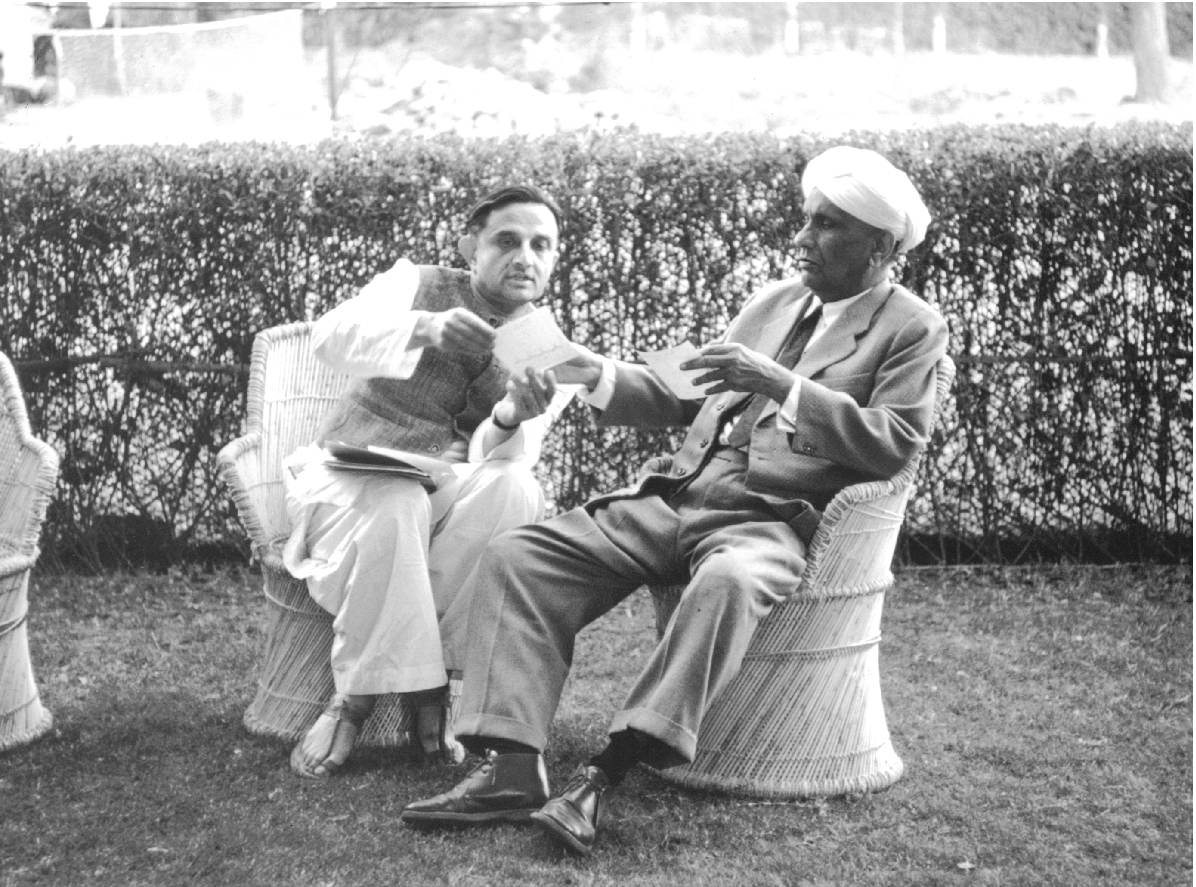
\includegraphics[scale=0.22]{"images/11.jpg"}
\caption{ಇಂಡಿಯನ್ ಅಕಾಡೆಮಿ ಆಫ್ ಸೈನ್ಸಸ್‍ನ ವಾರ್ಷಿಕ ಸಭೆ \enginline{1968}ರಲ್ಲಿ ಅಹಮದಾಬಾದಿನಲ್ಲಿ ನಡೆದಾಗ ವಿಕ್ರಂ ಸಾರಾಭಾಯ್ ಜೊತೆ ಸಿ. ವಿ. ರಾಮನ್. ರಾಮನ್ ರವರ \enginline{80}ನೇ ಹುಟ್ಟುಹಬ್ಬದ ಸಂಬಂಧವಾಗಿ ಅಭಿನಂದನೆ ಸಲ್ಲಿಸಲಾಯಿತು.}\label{chap2-fig02}
\end{figure}

ಫಿಸಿಕಲ್ ಲ್ಯಾಬ್ನ ಹುಲ್ಲುಗಾವಲಿನಲ್ಲಿ ರಾಮನ್‍ರನ್ನು ಅಭಿನಂದಿಸಲು ಸಂಜೆಯ ಔತಣಕೂಟ ಏರ್ಪಡಿಸಿದ್ದರು. ರಾಮನ್‍ರವರು ಕೇಂದ್ರ ಬಿಂದುವಾಗಿ ಸುತ್ತಲೂ ಶ್ರೇಷ್ಠ ವಿಜ್ಞಾನಿಗಳು ಕುಳಿತಿದ್ದರು. ರಾಮನ್‍ರವರ ಹಳೆಯ ವಿದ್ಯಾರ್ಥಿಗಳೂ ಇದ್ದರು. ಔತಣದ ನಂತರ ಅನೇಕ ವಿಜ್ಞಾನಿಗಳು ರಾಮನ್ ರವರನ್ನು ಹೊಗಳಿದರು. ಕೆಲವರು ತಮ್ಮ ವೃತ್ತಿ ಜೀವನಕ್ಕೆ ರಾಮನ್ ರವರ ಕೊಡುಗೆಯನ್ನು ನೆನೆದರು. ರಾಮನ್‍ರವರ ವೈಜ್ಞಾನಿಕ ಹಿರಿಮೆಯನ್ನು ಕೊಂಡಾಡಿದರು. ನನಗೆ ನೆನಪಿರುವಂತೆ\break ಜಿ. ಎನ್. ರಾಮಚಂದ್ರನ್‍ರವರಿಗೆ ಎರಡು ಮೂರು ವಾಕ್ಯಗಳಷ್ಟೇ ಮಾತನಾಡಲು ಸಾಧ್ಯವಾಯಿತು. ಅವರು ಅತಿ ಭಾವುಕರಾಗಿ ಕುಳಿತು ಬಿಟ್ಟರು. ಕೊನೆಗೆ ರಾಮನ್ ಉತ್ತರಿಸಿದರು.

 \enginline{-}“ನಾನು ಈ ಕಾಲದಲ್ಲೂ, ಈ ವಯಸ್ಸಿನಲ್ಲೂ ಈ ರುಮಾಲನ್ನು ಧರಿಸುವುದೇಕೆ ಎಂದು ಆಶ್ಚರ್ಯ ಪಡುತ್ತಿರಬಹುದು. ಏಕೆಂದು ನಾನು ಹೇಳುತ್ತೇನೆ. ನೀವು ನುಡಿದ ಹೊಗಳಿಕೆಗಳಿಗೆ ನನ್ನ ತಲೆ ಎಲ್ಲಿ ಉಬ್ಬಿ ಹೋಗುವುದೋ ಎಂದು ನಾನು ತಲೆಪಾಗು ಸುತ್ತಿ ಭದ್ರ ಪಡಿಸಿದ್ದೇನೆ....” “ಹೀಗೆ ಹೇಳಿ ತಲೆ ಎತ್ತಿ ಮರ, ಗಿಡ ಆಕಾಶ, ತಾರೆಗಳನ್ನು ನೋಡಿದರು. ಪ್ರಕೃತಿಯ ಅದ್ಭುತಗಳ ಬಗ್ಗೆ ಮಾತನಾಡತೊಡಗಿದರು. ಒಬ್ಬ ವಿಜ್ಞಾನಿಗೆ ಆಗುವ ಕುತೂಹಲವೂ ವೈಜ್ಞಾನಿಕ ಸತ್ಯದ ಅನ್ವೇಷಣೆಯು ನೀಡುವ ವಿನಯವನ್ನೂ ಕುರಿತು ಹೇಳಿದರು. ತಿಳಿದುಕೊಳ್ಳುವುದು ಮತ್ತು ಅಧ್ಯಯನ ಮಾಡುವುದು ಎಷ್ಟೊಂದಿದೆಯೆಂದರೆ ತಾವು ಏನನ್ನೂ ಮಾಡಲಾಗಿಲ್ಲವೆಂದರು. 

ಪ್ಯಾಸ್ಕಲ್ ಹೇಳಿಕೆಯನ್ನು ಜ್ಞಾಪಿಸಿಕೊಂಡರು\enginline{-} “ವ್ಯೋಮದಲ್ಲಿನ ಗೋಳದಂತೆ ಜ್ಞಾನವಿದೆ. ಅದರ ಗಾತ್ರ ಹೆಚ್ಚಿದಷ್ಟೂ, ಅರಿವಿಗೆ ಸಿಗದ ವಿಷಯಗಳ ಸಂಪರ್ಕ ಹೆಚ್ಚುತ್ತದೆ.”

 “ನೀವೆಲ್ಲ ನನ್ನ ಕೆಲಸದ ಬಗ್ಗೆ ಮತ್ತು ನನ್ನ ಸಾಧನೆಗಳ ಬಗ್ಗೆ ಮಾತನಾಡಿದ್ದೀರಿ. ಆದರೆ ನನಗೆ ತೃಪ್ತಿಯಿಲ್ಲ. ಐನ್‍ಸ್ಟೈನ್ ರಂತಹವರ ಮುಂದೆ ನಾನು ಎಲ್ಲಿದ್ದೇನೆ.” ಜೀವನದ ವಿದ್ಯಮಾನಗಳನ್ನು ಅರಿತುಕೊಳ್ಳಲು ಆಧುನಿಕ ಜೀವಶಾಸ್ತ್ರ ಸಂಶೋಧನೆಗೆ ಇತ್ತೀಚೆಗೆ ಒದಗಿರುವ ಸವಲತ್ತುಗಳ ಬಗ್ಗೆ ರಾಮನ್ ಹೇಳಿದರು. ಅಲ್ಲಿ ನೆರೆದಿರುವ ಮೇಲೆ ಈ ಮಾತುಗಳು ಬಹಳ ಪರಿಣಾಮ ಬೀರಿದವು.

ರಾಮನ್‍ರವರು ಕಡೆಗೆ ಒಂದು ಸಂಸ್ಥೆಯೇ ಆಗಿ ಬಿಟ್ಟರು. ಅವರ ಒಂಟಿತನ ಹೆಚ್ಚಿದಂತೆಲ್ಲಾ ಅವರಾಯಿತು, ಅವರ ಕೆಲಸವಾಯಿತು. ಅವರಿಗೆ ಖಾಯಿಲೆಯಾದಾಗ ಹಾಸಿಗೆ ಹಿಡಿದರು. ಅಲ್ಲಿಂದಲೇ ಡಾಕ್ಟರಿಗೆ ಹೇಳಿದರು\enginline{-} “ನಾನು ಖಾಯಿಲೆಯಿಂದ ವಾಸಿಯಾದರೆ ಮೊದಲಿನಂತೆ\break ಕೆಲಸಮಾಡುವಂತೆ ಆಗಬೇಕು. ಇಲ್ಲದಿದ್ದರೆ ಬದುಕಲು ಇಚ್ಛಿಸುವುದಿಲ್ಲ”. ಮರಣಕ್ಕೆ ಎರಡು ತಿಂಗಳ ಹಿಂದೆ (\enginline{2-10-70}), ಚಿಕ್ಕ ಹುಡುಗನ ರೀತಿಯ ಉತ್ಸಾಹದಲ್ಲಿ ಮೆಟ್ಟಲು ಹತ್ತಿ, ಮೊದಲನೇ ಮಹಡಿಯಲ್ಲಿ ಗಾಂಧಿ ಸ್ಮಾರಕದಲ್ಲಿ ಕೇಳುಮೆಯ (\enginline{Hearing}) ಸಿದ್ಧಾಂತದ ಬಗ್ಗೆ ಉಪನ್ಯಾಸವನ್ನು ನೀಡಿದರು. ಇದು ರಾಮನ್‍ರವರ ಕೊನೆಯ ಉಪಾನ್ಯಾಸವಾಗಿತ್ತು. ಅವರ ವಿಷಯ ವಿಸ್ತಾರವನ್ನೂ ಮತ್ತು ಅವರ ಅಧ್ಯಯನದ ಆಳವನ್ನೂ ಈ ಉಪನ್ಯಾಸವು ಎತ್ತಿ ತೋರಿಸುತ್ತದೆ. ಕೊನೆಯವರೆಗೂ ಹೊಸದನ್ನು ಕಲಿಯುತ್ತಾ ಅಧ್ಯಯನ ಮಾಡುತ್ತಾ, ದಣಿವರಿಯದೆ ಕೆಲಸ ಮಾಡುವ ಅವರ\break ಜಾಯಮಾನವನ್ನು ತೆರೆದಿಡುತ್ತದೆ.

ನಾನು ನನ್ನ ವೃತ್ತಿಯಿಂದ ಬಿಡುವು ಪಡೆದುಕೊಂಡು ಒಂದು ವರ್ಷದ ಮಟ್ಟಿಗೆ ಭಾರತಕ್ಕೆ ಬಂದೆ. ನಾನು ಭಾರತದಲ್ಲಿ ಹೈ ಪ್ರೆಶರ್ ರಿಸರ್ಚ್‌ಗೆ ವ್ಯವಸ್ಥೆ ಮಾಡಲು ಬಂದಿದ್ದೆ. ನಾನು ಬಂದೊಡನೆ ಗುರುಗಳಿಗೆ ನಮನ ಸಲ್ಲಿಸಲು ಹೊರಟೆ. \enginline{1968} ಡಿಸೆಂಬರ್ ನಲ್ಲಿ ಅಹಮದಾಬಾದಿನಲ್ಲಿ ಕಂಡಾಗ ಬಹಳ ಬೇಗ ದಣಿಯುತ್ತಿದ್ದರು. ಜನವರಿ \enginline{1969} ರಿಂದ ಅಕ್ಟೋಬರ್ \enginline{1970} ರ ಅವಧಿಯಲ್ಲಿ ಅನೇಕ ಬಾರಿ ಆನಾರೋಗ್ಯ ಪೀಡಿತರಾಗಿದ್ದರು. ಹಿಂದಿನ ಕಸುವು ಇರಲಿಲ್ಲ. ನಾನು ಅವರ ಬಂಗಲೆಗೆ ಹೋದೆ. ಲೇಡಿ ರಾಮನ್ ಬೇಡವೆಂದರೂ, ಅವರು ನನ್ನೊಡನೆ ಮಾತನಾಡಲು ಎದ್ದು ಕುಳಿತರು. ಇದೇ ನನ್ನ ಕೊನೆಯ ಸಂಭಾಷಣೆ. ಇದಾದ ಬಳಿಕ ಹೃದಯಾಘಾತವಾಗಿ ಆಸ್ಪತ್ರೆ ಸೇರಿದರು. ಕೊಂಚ ಸುಧಾರಿಸಿಕೊಂಡರೂ ಕೆಲವೇ ದಿನಗಳಲ್ಲಿ ತೀರಿಕೊಂಡರು. ನವೆಂಬರ್ \enginline{21, 1970} ಶನಿವಾರ ಬೆಳಗಿನ ಜಾವ ಅವರು ತೀರಿಕೊಂಡರು. ಪರವಾನಗಿ ಪಡೆದು ರಾಮನ್ ಸಂಸ್ಥೆಯ ಆವರಣದಲ್ಲೇ ಅವರ ಅಂತ್ಯಕ್ರಿಯೆ ಮಾಡಲಾಯಿತು. ಸಾವಿರಾರು ನಾಗರಿಕರು, ವಿಜ್ಞಾನಿಗಳು, ವಿದ್ಯಾರ್ಥಿಗಳು, ಸಂಸ್ಥೆಯ ಆವರಣದಲ್ಲಿ ನೆರೆದು ಶ್ರದ್ಧಾಂಜಲಿ ಅರ್ಪಿಸಿದರು.

ಸಾವು ಅನಿವಾರ್ಯ, ಆದರೆ ನಿಮ್ಮ ಜೀವನ ರೂಪಿಸಿ ಅದಕ್ಕೊಂದು ಮೌಲ್ಯ ನೀಡಿದವರಿಗೆ ಸಾವು ಬರುವುದು ಬೇಡ ಎನಿಸುತ್ತದೆ. ನಾನು ಅವರು ಪ್ರಕೃತಿಲೀನರಾದಾಗ ಇಲ್ಲಿದ್ದೆ ಎನ್ನುವುದಷ್ಟೇ ಸಮಾಧಾನ. ನನ್ನೊಳಗೆ ನಿಶ್ಶಬ್ದ ರೋದನವಿತ್ತು. ನಾನು ಅವರು ಪ್ರಕೃತಿಲೀನರಾದಾಗ ಇರದಿದ್ದರೆ ಬಹಳ ಬೇಸರ ಪಡುತ್ತಿದ್ದೆ. ಚಂದ್ರಶೇಖರ ವೆಂಕಟ ರಾಮನ್‍ರವರಿಗೆ ಶ್ರದ್ಧಾಂಜಲಿ ಅರ್ಪಿಸಿದ್ದು ನನಗೆ ಸಮಾಧಾನ ತಂದಿತ್ತು.

ಸಂಸ್ಥೆಯ ಡೈರೆಕ್ಟರಾಗಿ ರಾಮನ್‍ರವರ ಕೊನೆಯ ಮಗ ರೇಡಿಯೋ ವಿಜ್ಞಾನಿ ವಿ. ರಾಧಕೃಷ್ಣನ್ ನೇಮಕಗೊಂಡರು. ಕಳೆದ \enginline{16} ವರ್ಷಗಳಲ್ಲಿ ಸಂಸ್ಥೆಯು ಉದ್ದಗಲಗಳಲ್ಲಿ ಬೆಳೆದಿದೆ. ಖಭೌತಶಾಸ್ತ್ರ ಮತ್ತು ರೇಡಿಯೋ ಖಗೋಳವಿಜ್ಞಾನಗಳಲ್ಲಿ ಸಂಶೋಧನೆಗಳು ನಡೆಯುತ್ತಿವೆ. ರಾಮನ್\break ಊಹಿಸಿದ್ದಕ್ಕಿಂತಲೂ ಬೃಹತ್ತಾಗಿ ಸಂಸ್ಥೆಯ ಹಣಕಾಸು ವೃದ್ಧಿಯಾಗಿದೆ. ಸರ್ಕಾರವು ಹೆಚ್ಚಿನ ಅನುದಾನ ನೀಡುತ್ತಿದೆ.

\begin{sidewaysfigure}[!htbp]
\centering
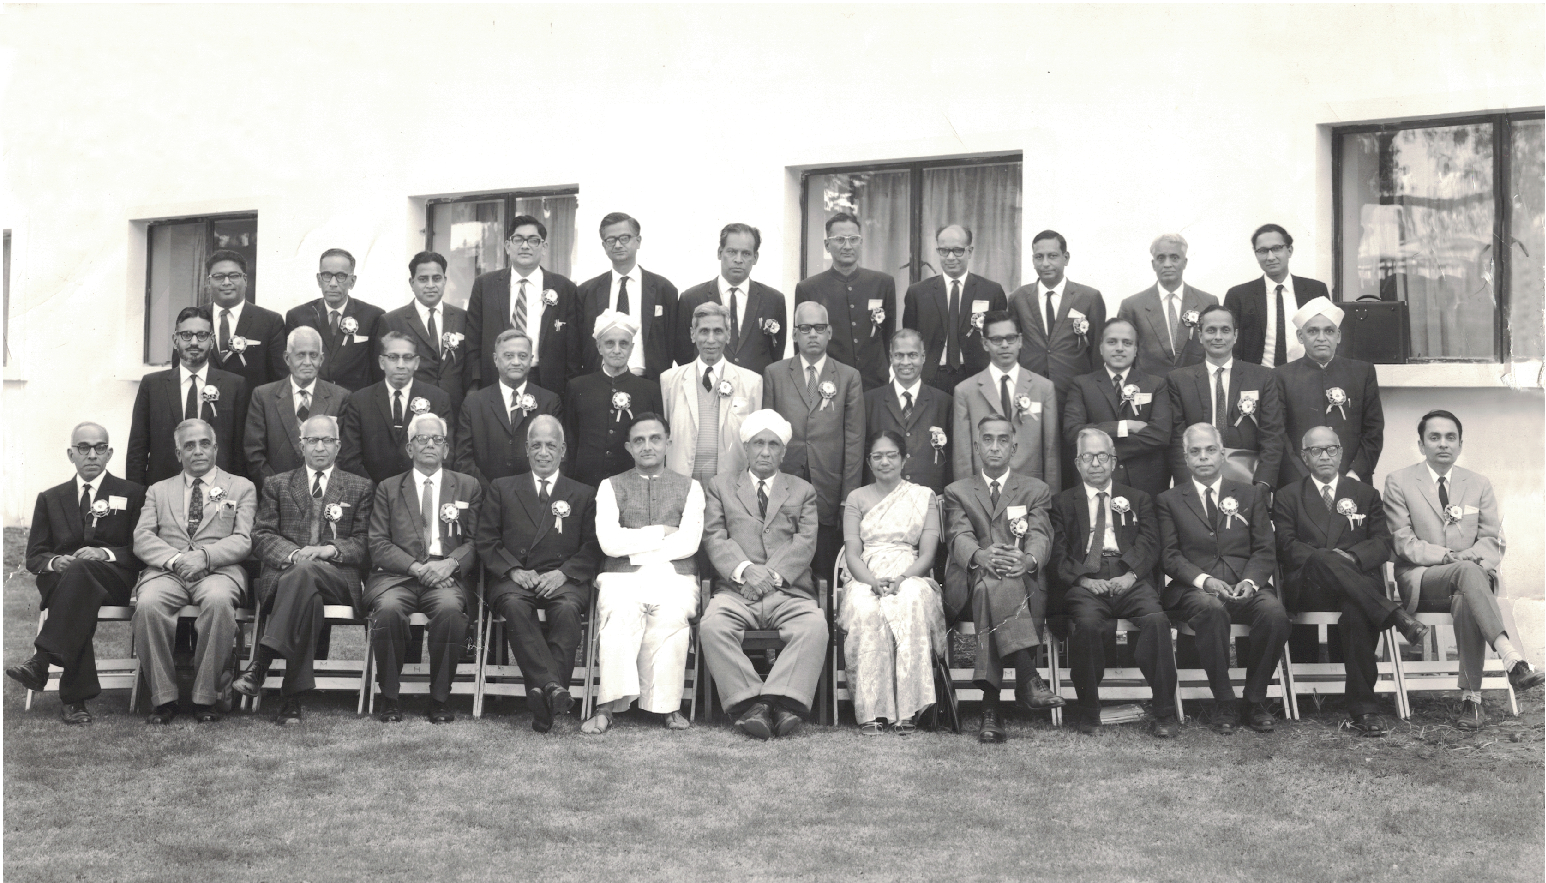
\includegraphics[scale=0.3]{"images/13.jpg"}
\caption{ ರಾಮನ್‌ರವರ \enginline{80}ನೇ ಹುಟ್ಟು ಹಬ್ಬದ ಆಚರಣೆ. ಅಹಮದಾಬಾದ್‌ನಲ್ಲಿ \enginline{1968}ರಲ್ಲಿ ಜರುಗಿದ ಭಾರತೀಯ ವಿಜ್ನಾನ ಅಕಾಡೆಮಿಯ ವಾರ್ಷಿಕ ಸಭೆ.}\label{chap2-fig03}
\end{sidewaysfigure}

